%==================================================================
% Ini adalah file utama dari dokumen LaTeX ini
%==================================================================

%% DILARANG EDIT BAGIAN INI
\documentclass[12pt, a4paper, onecolumn, oneside, final]{report}

%%========================================================================
%% WAJIB DIISI SESUAI DATA YANG BENAR DAN TIDAK BOLEH ADA YANG TERLEWAT
%%========================================================================

\providecommand{\judulid}{Analisis Performa Quadcopter dengan Penerapan Algoritma Kendali Pid pada Kontroler Penerbangan blablabla blablabla blablabla} %Judul Tugas Akhir Bahasa Indonesia
\providecommand{\judulen}{Quadcopter Performance Analysis with the Application of the Pid Control Algorithm on the Flight Controller blablabla blablabla blablabla} %Judul Tugas Akhir Bahasa Inggirs
\providecommand{\penulis}{Bintang Chen Sudiro Hutama Karya} %Nama Lengkap Mahasiswa 
\providecommand{\nim}{10293847564738} % NIM

\providecommand{\tipe}{Tugas Akhir} %Tipe Laporan
\providecommand{\type}{Undergraduate Thesis} %Tipe Laporan
\providecommand{\prodi}{Sarjana Terapan Teknik Elektronika} %Nama Prodi
\providecommand{\fakultas}{Fakultas Vokasi} %Nama Fakultas
\providecommand{\universitas}{Universitas Negeri Yogyakarta} %Nama Universitas

\providecommand{\tglpersetujuan}{15 Juli 2023} %Tanggal di Lembar Persetujuan
\providecommand{\tglpernyataan}{\today} %Tanggal di Surat Pernyataan
\providecommand{\tglpengesahan}{\today} %Tanggal di Halaman Pengesahan
\providecommand{\tahun}{\the\year{}} %Tahun Proyek Akhir

\providecommand{\pembimbing}{Ir. Ardy Seto Priambodo, S.T., M.Eng.} %Nama Dosen Pembimbing
\providecommand{\NIPpembimbing}{198906052019031014} %NIP Dosen Pembimbing

\providecommand{\sekretaris}{Dr. Aris Nasuha, S.Si., M.T.} %Nama Sekretaris Penguji
\providecommand{\penguji}{Oktaf Agni Dhewa, S.Si., M.Cs.} %Nama Penguji

\providecommand{\tglpengesahanketua}{15 Juli 2023} %Tanggal di Lembar Pengesahan oleh Ketua Penguji
\providecommand{\tglpengesahansekretaris}{\today} %Tanggal di Lembar Pengesahan oleh Ketua Penguji
\providecommand{\tglpengesahanpenguji}{15 Juli 2023} %Tanggal di Lembar Pengesahan oleh Ketua Penguji

\providecommand{\dekan}{Prof. Dr. Komarudin, S.Pd., M.A.} %Nama Dekan
\providecommand{\NIPdekan}{197409282003121002} %NIP Dekan

\providecommand{\koorprodi}{Dr. Aris Nasuha, S.Si., M.T.} %Nama Koorprodi
\providecommand{\NIPkoorprodi}{196906151994031002} %NIP Koorprodi

\providecommand{\katakunci}{Konsep Abstrak, Komponen Abstrak, Kata Kunci.} %Kata kunci dalam Bahasa Indonesia
\providecommand{\keywords}{Abstract Concepts, Abstract Components, Key Words.} %Kata kunci dalam Bahasa Inggris

%% Daftar Nama Dosen Pembimbing
%%
%% Dr. Aris Nasuha, S.Si., M.T.
%% 196906151994031002
%%
%% Ir. Ardy Seto Priambodo, S.T., M.Eng.
%% 198906052019031014
%%
%% Arya Sony, S.T., M.Eng.
%% 199109172018031001
%%
%% Purno Tri Aji, S.T., M.Eng.
%% 198410092010121001
%%
%% Ir. Oktaf Agni Dhewa, S.Si., M.Cs.
%% 12009911024719
%%
%% Gilang Nugraha Putu Pratama, S.Si., M.Eng.
%% 12107900406786
%==================================================================
% Konfigurasi utama untuk dokumen LaTeX
%==================================================================

%% DILARANG EDIT BAGIAN INI

% Mengatur bahasa dokumen ke Bahasa Indonesia dan encoding karakter
\usepackage[indonesian]{babel}
\usepackage[utf8]{inputenc}

% Pengaturan jarak antar baris dan penyesuaian kotak teks agar rata kiri
\usepackage{setspace}
\usepackage[raggedrightboxes]{ragged2e}

% Paket untuk memasukkan gambar dalam dokumen
\usepackage{graphicx}
\graphicspath{{gambar/}} % Menentukan folder default untuk gambar
\usepackage{float}       % Mengatur posisi gambar dalam teks

% Mengatur indentasi paragraf
\usepackage{indentfirst}  % Memastikan paragraf pertama di setiap section memiliki indentasi
\setlength\parindent{1cm} % Mengatur jarak indentasi paragraf menjadi 1 cm

% Mengatur font utama dokumen menjadi Times New Roman
\usepackage{pslatex}

% Mengatur format penomoran section dan subsection
\renewcommand{\thesection}{\Alph{section}.\hspace{0.18cm}} % Section: A, B, C, ...
\renewcommand{\thesubsection}{\arabic{subsection}.}         % Subsection: 1, 2, 3, ...

% Pengaturan daftar isi, daftar gambar, dan daftar tabel
\usepackage{tocloft}
\cftsetpnumwidth{1.5em}
\cftsetrmarg{2em}
\setlength{\cftsecnumwidth}{1.5em}
\setlength{\cftsubsecnumwidth}{1.5em}
\renewcommand{\cftchapdotsep}{\cftdotsep}
\setlength{\cftbeforechapskip}{3pt}

% Penyesuaian judul bab dalam daftar isi agar ditampilkan sebagai "BAB"
\renewcommand\cftchappresnum{BAB }
\renewcommand\cftchapaftersnum{}
\newlength\mylen
\settowidth\mylen{\bfseries BAB 1 :\ } % Menyesuaikan lebar penomoran bab
\cftsetindents{chap}{0pt}{\mylen}

% Pengaturan format dan penomoran judul bab
\usepackage{titlesec}
\titleformat{\chapter}{\doublespacing\fontsize{14pt}{16pt}\bfseries}{\MakeUppercase{\chaptertitlename\ \Roman{chapter}}\filcenter}{0.15cm}{\centering\uppercase}
\titleformat{\section}{\fontsize{12}{14}\bfseries}{\thesection}{0.4cm}{}
\titleformat{\subsection}{\fontsize{12}{14}\bfseries}{\thesubsection}{0.675cm}{}

% Mengatur jarak dan format spacing untuk chapter, section dan subsection
\titlespacing*{\chapter}{0pt}{-1cm}{20pt}
\titlespacing*{\section}{0pt}{10pt}{0cm}
\titlespacing*{\subsection}{0pt}{10pt}{0cm}

% Pengaturan untuk caption gambar dan tabel
\usepackage[font=small, format=plain, labelfont=bf, up, textfont=up]{caption}
\usepackage{subcaption}

% Menghapus tanda titik dua pada caption
\captionsetup[figure]{labelsep=space}
\captionsetup[table]{labelsep=space}

% Mengatur nomor caption gambar dan tabel sesuai bab
\renewcommand{\thefigure}{\arabic{chapter}.\arabic{figure}}
\renewcommand{\thetable}{\arabic{chapter}.\arabic{table}}

% Mengatur hyphenation (pemisahan kata) agar lebih rapi
\tolerance=1
\emergencystretch=\maxdimen
\hyphenpenalty=10000
\hbadness=10000

% Pengaturan tabel, multirow, dan ukuran kolom otomatis
\usepackage{tabularx}
\usepackage{multirow}

% Pengaturan margin halaman
\usepackage{geometry}
\geometry{
    left=4cm,          % Margin kiri
    top=3cm,           % Margin atas
    right=3cm,         % Margin kanan
    bottom=3cm,        % Margin bawah
}

% Paket untuk notasi matematika
\usepackage{amsmath}

% Pengaturan nomor pada persamaan matematika sesuai bab
\renewcommand{\theequation}{\arabic{chapter}.\arabic{equation}}

% Untuk halaman berorientasi landscape
\usepackage{rotating}

% Pengaturan untuk list (daftar item dan angka)
\usepackage{enumitem}
\setlist{nosep} % Menghilangkan jarak antar item dalam list
\newenvironment{packed_enum}{ % Membuat lingkungan untuk daftar bernomor
    \begin{enumerate}[leftmargin=1.5\parindent]
        \setlength{\itemsep}{0pt}
        \setlength{\parskip}{0pt}
        \setlength{\parsep}{0pt}
        }{\end{enumerate}}

\newenvironment{packed_item}{ % Membuat lingkungan untuk daftar berpoin
    \begin{itemize}[leftmargin=1.375\parindent]
        \setlength{\itemsep}{0pt}
        \setlength{\parskip}{0pt}
        \setlength{\parsep}{0pt}
        }{\end{itemize}}

% Paket untuk bibliografi menggunakan BibTeX
\usepackage[sort]{natbib}
\bibliographystyle{newapa} % Ganti dengan apalike jika menggunakan Overleaf

% Paket untuk tabel yang panjang dan melampaui satu halaman
\usepackage{longtable}

% Paket untuk memasukkan hyperlink dalam dokumen
\usepackage{hyperref}

% Pengaturan label otomatis untuk berbagai elemen (gambar, tabel, persamaan)
\usepackage{cleveref}
\crefname{figure}{gambar}{gambar}
\Crefname{figure}{Gambar}{Gambar}
\crefname{table}{tabel}{tabel}
\Crefname{table}{Tabel}{Tabel}
\crefname{equation}{persamaan}{persamaan}
\Crefname{equation}{Persamaan}{Persamaan}
\crefname{lstlisting}{kode}{kode}
\Crefname{lstlisting}{Kode}{Kode}

%\AtBeginDocument{\renewcommand{\lstlistingname}{Kode}} 
%\AtBeginDocument{\renewcommand{\thelstlisting}{\thechapter.\arabic{lstlisting}}}
%\AtBeginDocument{\renewcommand{\thelstlisting}{\arabic{chapter}.\arabic{lstlisting}.}}
\AtBeginDocument{\renewcommand{\lstlistingname}{Kode}}
\AtBeginDocument{\renewcommand{\thelstlisting}{\arabic{chapter}.\arabic{lstlisting}}}

\captionsetup[lstlisting]{
  format=plain,
  labelfont=bf,
  justification=centering,
  singlelinecheck=false,
  labelsep=space
}

% Paket untuk menampilkan kode program
\usepackage{listings}
\usepackage{xcolor}
\definecolor{codegreen}{rgb}{0,0.6,0}
\definecolor{codegray}{rgb}{0.5,0.5,0.5}
\definecolor{codepurple}{rgb}{0.58,0,0.82}
\definecolor{backcolour}{rgb}{0.95,0.95,0.92}
\lstdefinestyle{mystyle}{
    backgroundcolor=\color{backcolour},   
    commentstyle=\color{codegreen},
    keywordstyle=\color{magenta},
    numberstyle=\tiny\color{codegray},
    stringstyle=\color{codepurple},
    basicstyle=\ttfamily\footnotesize,
    columns=fullflexible,
    breakatwhitespace=false,         
    breaklines=true,                 
    captionpos=b,                    
    keepspaces=true,                 
    numbers=left,                    
    numbersep=5pt,                  
    showspaces=false,                
    showstringspaces=false,
    showtabs=false,                  
    tabsize=2,
    lineskip=-1pt
}
\lstset{style=mystyle}

%paket untuk gambar dengan tikz
\usepackage{tikz}
\usepackage{pgfplots}
\usepackage{pgf-pie}
\pgfplotsset{compat=1.18}
\usetikzlibrary{shapes.geometric, arrows}
\tikzstyle{startstop} = [rectangle, rounded corners, minimum width=3cm, minimum height=1cm,text centered, draw=black, fill=red!30]
\tikzstyle{process} = [rectangle, minimum width=3cm, minimum height=1cm, text centered, draw=black, fill=orange!30]
\tikzstyle{decision} = [diamond, minimum width=3cm, minimum height=1cm, text centered, draw=black, fill=green!30]
\tikzstyle{arrow} = [thick,->,>=stealth]

%untuk if-then
\usepackage{ifthen}
%% DILARANG EDIT BAGIAN INI
%% Ini adalah daftar kata yang terpotong, kadang kala LaTeX tidak memenggal kata dengan benar
%% sehingga harus ditambahkan kata yang terpotong tersebut di bagian ini
%% silahkan menyesuaikan kebutuhan apabila dibutuhkan
%tulis seperlunya, kalau menemukan kata yang terpenggal salah, misalnya.. 
\hyphenation{be-ri-kut}
\hyphenation{a-da-lah}

%\newcommand{\Jenis}{Proposal} %Pilih salah satu antara Proposal atau Laporan
\newcommand{\Jenis}{Laporan} %Pilih salah satu antara Proposal atau Laporan

\begin{document}
\ifthenelse{\equal{\Jenis}{Proposal}}{
	%==================================================================
% Ini adalah sampul luar
%==================================================================

%% DILARANG EDIT BAGIAN INI

\begin{titlepage}
    \begin{center}

        \begin{doublespace}
            \textbf{\Large{\MakeUppercase{\judulid}}}\\[2cm]
        \end{doublespace}
        \textbf{\MakeUppercase{\large{Proposal \tipe}}}\\[0.5cm]

        Diajukan Sebagai Syarat Untuk Pengajuan Tugas Akhir Pada Program Studi Teknik Elektronika {\fakultas} {\universitas}\\[1.5cm]

        
\includegraphics[width=0.3\linewidth]{gambar/logo-uny.png}\\[1.5cm]

        \textbf{Oleh:} \\
        \textbf{\MakeUppercase{{\penulis}}} \\
        \textbf{NIM} \textbf{{\nim}}\\[2cm]

        \vfill

        \textbf{\large \MakeUppercase{Prodi \prodi}}\\
        \textbf{\large \MakeUppercase{\fakultas}}\\
        \textbf{\large \MakeUppercase{\universitas}}\\
        \textbf{\large \the\year{}}\\
    \end{center}
\end{titlepage}

%% DILARANG EDIT BAGIAN INI
	\pagenumbering{roman}
	%==================================================================
% Ini adalah sampul dalam
%==================================================================

%% DILARANG EDIT BAGIAN INI
\newpage
\addcontentsline{toc}{chapter}{HALAMAN SAMPUL}
\begin{center}
    \begin{doublespace}
        \textbf{\large{\MakeUppercase{\judulid}}}\\[2.5cm]
    \end{doublespace}

    \textbf{\MakeUppercase{\large{Proposal \tipe}}}\\[0.5cm]
    \begin{onehalfspace}
        Diajukan kepada {\fakultas} {\universitas} Sebagai Syarat Untuk Pengajuan Tugas Akhir Pada Program Studi Teknik Elektronika\\[1.8cm]
    \end{onehalfspace}

    \large Oleh: \\
    \begin{onehalfspace}
        \large{\penulis} \\
        \large{\nim}\\[1.5cm]
    \end{onehalfspace}
    \vspace{1.5cm}

    \large Pembimbing: \\
    \begin{onehalfspace}
        \large{\pembimbing} \\
    \end{onehalfspace}

    \vfill

    \textbf{\large \MakeUppercase{Prodi \prodi}}\\
    \textbf{\large \MakeUppercase{\fakultas}}\\
    \textbf{\large \MakeUppercase{\universitas}}\\
    \textbf{\large \the\year{}}\\
\end{center}
%% DILARANG EDIT BAGIAN INI
	%==================================================================
% Ini adalah halaman persetujuan
%==================================================================

%% DILARANG EDIT BAGIAN INI
\newpage
\addcontentsline{toc}{chapter}{LEMBAR PERSETUJUAN PROPOSAL}
\begin{center}
    \begin{doublespace}
        \textbf{\large \MakeUppercase{lembar persetujuan}}
    \end{doublespace}
\end{center}

\begin{center}
    Proposal {\tipe} dengan Judul
\end{center}

\begin{center}
    \begin{doublespace}
        \textbf{\large \MakeUppercase {\judulid}}
    \end{doublespace}
\end{center}

\begin{center}
    Disusun oleh:\\
    \textbf{\penulis}\\
    \textbf{NIM \nim}\\[1.5cm]

    telah memenuhi syarat dan disetujui oleh Dosen Pembimbing untuk dilaksanakan Seminar Proposal {\tipe} bagi yang bersangkutan.\\[0.75cm]
\end{center}

\begin{minipage}{0.35\textwidth}
    \hfill\\[2em]
    Mengetahui,\\
    Koordinator Program Studi,\\[2cm]
    \resizebox{\textwidth}{!}{\koorprodi}\\
    NIP. \NIPkoorprodi
\end{minipage}
\hfill
\begin{minipage}{0.47\textwidth}
    Wates, \tglpersetujuan\\[1em]
    Disetujui,\\
    Dosen Pembimbing TA,\\[2cm]
    \resizebox{\textwidth}{!}{\pembimbing}\\
    NIP. \NIPpembimbing
\end{minipage}%
%% DILARANG EDIT BAGIAN INI

	\begin{spacing}{1.2}
		%% DILARANG EDIT BAGIAN INI
% Daftar Isi
\clearpage
\phantomsection
\addcontentsline{toc}{chapter}{DAFTAR ISI}
%\renewcommand{\cftdotsep}{\cftnodots}
\setlength{\cftbeforetoctitleskip}{-0.5cm}
\renewcommand{\cfttoctitlefont}{\hfill\large\bfseries}
\renewcommand{\cftaftertoctitle}{\hfill\hfill}
\renewcommand\contentsname{DAFTAR ISI}
\singlespacing
\tableofcontents

% Daftar Singkatan
%% DILARANG EDIT BAGIAN INI
\clearpage
\phantomsection
\addcontentsline{toc}{chapter}{DAFTAR SINGKATAN}

\begin{center}
    \large \textbf{DAFTAR SINGKATAN}
\end{center}
\vspace{3em}
%% DILARANG EDIT BAGIAN INI

%% edit bagian ini
\begin{center}
    \begin{table}[hb]
        \begin{tabular}{|l|l|}
        \hline
        \textbf{Notasi} & \textbf{Arti}                    \\ \hline
        FWHM            & \textit{Full width half maximum} \\ \hline
        rms             & \textit{root mean square}        \\ \hline
        RFS             & \textit{Rotary forcespinning}    \\ \hline
        PVP             & Polivinil pirolidon              \\ \hline
        SI              & Satuan Internasional             \\ \hline
        SI              & Satuan Internasional             \\ \hline
        SI              & Satuan Internasional             \\ \hline
        SI              & Satuan Internasional             \\ \hline
        SI              & Satuan Internasional             \\ \hline
        SI              & Satuan Internasional             \\ \hline
        SI              & Satuan Internasional             \\ \hline
        SI              & Satuan Internasional             \\ \hline
        SI              & Satuan Internasional             \\ \hline
        SI              & Satuan Internasional             \\ \hline
        \end{tabular}
        \end{table}
\end{center}
%% edit bagian ini

% Daftar Gambar
\clearpage
\phantomsection
\addcontentsline{toc}{chapter}{DAFTAR GAMBAR}
\setlength{\cftbeforeloftitleskip}{-0.5cm}
\renewcommand{\cftloftitlefont}{\hfill\large\bfseries}
\renewcommand{\cftafterloftitle}{\hfill}
\renewcommand{\cftfigleader}{\dotfill}
\renewcommand\listfigurename{DAFTAR GAMBAR}
\listoffigures

% Daftar Tabel
\clearpage
\phantomsection
\addcontentsline{toc}{chapter}{DAFTAR TABEL}
\setlength{\cftbeforeloftitleskip}{-0.5cm}
\renewcommand{\cftloftitlefont}{\hfill\large\bfseries}
\renewcommand{\cftafterloftitle}{\hfill}
\renewcommand{\cfttableader}{\dotfill}
\renewcommand\listtablename{\centerline {\large\bfseries  DAFTAR TABEL}}
\listoftables
%% DILARANG EDIT BAGIAN INI
	\end{spacing}

	\pagenumbering{arabic}

	\begin{spacing}{1.5}
		%==================================================================
% Ini adalah bab 1
% Silahkan edit sesuai kebutuhan, baik menambah atau mengurangi \section, \subsection
%==================================================================

\chapter[PENDAHULUAN]{\\ PENDAHULUAN}

\section{Latar Belakang}
Bagian ini menjelaskan alasan dan motivasi di balik pengembangan proyek ini. Proyek ini diinisiasi untuk mengatasi kebutuhan atau permasalahan tertentu yang timbul dalam bidang teknologi, industri, atau aplikasi sehari-hari. Melalui identifikasi kebutuhan ini, diperoleh wawasan tentang bagaimana proyek dapat memberikan solusi yang efektif dan efisien. Latar belakang ini juga menguraikan pentingnya topik proyek dalam perkembangan teknologi terkini, serta bagaimana penerapan teknologi atau metode yang diusulkan dapat membawa nilai tambah. Selain itu, bagian ini memberikan gambaran singkat mengenai situasi atau tren teknologi saat ini yang mempengaruhi pengembangan proyek.

\section{Rumusan Masalah}
Rumusan masalah adalah langkah penting yang merangkum permasalahan spesifik atau kebutuhan yang menjadi dasar pengembangan proyek. Pada bagian ini, dijelaskan permasalahan utama yang dihadapi, seperti keterbatasan pada sistem atau perangkat yang sudah ada, atau kebutuhan baru yang belum terpenuhi oleh teknologi saat ini. Identifikasi masalah juga mencakup tantangan teknis, fungsional, atau ekonomi yang menjadi penghambat dan bagaimana proyek ini diharapkan dapat menjawab permasalahan tersebut. Fokusnya adalah memberikan pemahaman yang jelas mengenai alasan pentingnya mengembangkan proyek ini sebagai solusi yang dibutuhkan.

\section{Tujuan Proyek}
Tujuan proyek menyatakan secara spesifik hasil atau capaian yang diinginkan dari pengembangan proyek ini. Bagian ini dirancang untuk memastikan bahwa proyek memiliki sasaran yang jelas dan terukur. Tujuan tersebut dirumuskan berdasarkan masalah yang telah diidentifikasi dan mencakup pencapaian tertentu, seperti peningkatan kinerja sistem, efisiensi, atau kemudahan penggunaan yang diharapkan. Selain itu, tujuan proyek dapat berupa pengembangan prototipe, penerapan teknologi tertentu, atau pencapaian fungsionalitas baru yang belum ada. Penjabaran tujuan yang jelas membantu menjaga fokus proyek dan memberikan arah yang tepat dalam setiap tahapan pengembangan.

\section{Manfaat Proyek}
Manfaat proyek menguraikan dampak positif yang diharapkan dari hasil proyek ini bagi pengguna, industri, atau masyarakat secara umum. Manfaat ini mencakup berbagai aspek, seperti kontribusi terhadap peningkatan produktivitas, pengurangan biaya, peningkatan kualitas, atau kemudahan dalam penggunaan teknologi. Selain manfaat langsung, proyek ini juga diharapkan memiliki dampak jangka panjang yang bermanfaat, seperti mendorong inovasi di bidang terkait atau membuka peluang baru untuk pengembangan lebih lanjut. Dengan menjelaskan manfaat proyek, pembaca dapat memahami nilai tambah yang dihadirkan oleh proyek ini.

\section{Batasan Proyek}
Batasan proyek mengidentifikasi cakupan dan batasan ruang lingkup pengembangan sistem atau perangkat yang dirancang. Bagian ini mencakup aspek-aspek yang akan menjadi fokus utama dalam pengembangan serta aspek yang akan dikecualikan dari lingkup proyek. Penjelasan batasan ini penting agar proyek tetap terarah dan tidak meluas ke aspek-aspek yang berada di luar tujuan awal. Batasan proyek juga mencakup keterbatasan teknis, waktu, atau sumber daya yang mempengaruhi desain dan implementasi sistem. Dengan menetapkan batasan, proyek ini dapat lebih terfokus dan efisien dalam pencapaiannya.

\section{Keaslian Gagasan}
Keaslian gagasan bertujuan untuk menekankan inovasi atau kontribusi unik yang ditawarkan oleh proyek ini. Bagian ini menjelaskan bagaimana proyek ini menawarkan pendekatan yang berbeda atau peningkatan dibandingkan dengan metode atau perangkat yang sudah ada. Keaslian gagasan dapat diperlihatkan melalui perbandingan dengan proyek atau produk serupa, menunjukkan perbedaan signifikan atau keunggulan yang dihadirkan oleh solusi yang diusulkan. Misalnya, peningkatan kinerja, efisiensi, atau kemudahan penggunaan yang dihasilkan dari metode atau pendekatan baru. Selain itu, bagian ini juga bisa mencakup penggunaan teknologi atau desain yang belum banyak diterapkan dalam konteks yang sama. Penekanan pada keaslian gagasan membantu menunjukkan bahwa proyek ini tidak hanya mengikuti pola yang sudah ada, tetapi juga menghadirkan sesuatu yang baru dan relevan.

\section{Sistematika Penulisan}
Sistematika penulisan memberikan panduan mengenai struktur dari keseluruhan laporan proyek ini, sehingga memudahkan pembaca dalam memahami alur isi laporan dari setiap bab. Bagian ini menjelaskan isi dari setiap bab secara singkat, mulai dari latar belakang hingga kesimpulan dan rekomendasi. Misalnya, BAB I membahas pendahuluan dan dasar pengembangan proyek, BAB II menguraikan tinjauan pustaka dan landasan teori, dan seterusnya. Dengan memberikan sistematika penulisan, pembaca dapat memahami bagaimana laporan ini disusun secara keseluruhan dan bagaimana setiap bab saling berkaitan dalam mencapai tujuan akhir proyek.
		%==================================================================
% Ini adalah bab 2
% Silahkan edit sesuai kebutuhan, baik menambah atau mengurangi \section, \subsection
%==================================================================

\chapter[PENDEKATAN PEMECAHAN MASALAH]{\\ PENDEKATAN PEMECAHAN MASALAH}

\section{Dasar Teori 2.1}
Tinjauan pustaka berdasarkan teori dalam laporan proyek akhir sarjana terapan adalah bagian yang menjabarkan tentang teori yang relevan dengan masalah yang akan diteliti dalam proyek akhir sarjana terapan. Dalam tinjauan pustaka ini, peneliti harus mengumpulkan dan menganalisis sumber-sumber yang berkaitan dengan masalah yang akan diteliti, seperti buku, artikel ilmiah, jurnal, serta sumber-sumber online yang terpercaya.

Dalam tinjauan pustaka berdasarkan teori, peneliti harus menjelaskan :
\begin{packed_item}
    \item Teori-teori yang digunakan dalam penelitian
    \item Konsep-konsep yang digunakan dalam penelitian
    \item Kerangka teori yang digunakan dalam proyek akhir sarjana terapan
\end{packed_item}

Untuk contoh, dalam laporan proyek akhir sarjana terapan yang meneliti pengaruh perubahan iklim terhadap produktivitas tanaman padi, tinjauan pustaka berdasarkan teori harus menjelaskan teori-teori yang digunakan dalam penelitian, seperti teori perubahan iklim, teori produktivitas tanaman, serta teori adaptasi tanaman terhadap perubahan iklim.

Konsep-konsep yang digunakan dalam penelitian, seperti konsep perubahan iklim, konsep produktivitas tanaman, serta konsep adaptasi tanaman terhadap perubahan iklim.

Kerangka teori yang digunakan dalam proyek akhir sarjana terapan harus menjabarkan tentang hubungan antara perubahan iklim, produktivitas tanaman, serta adaptasi tanaman terhadap perubahan iklim.

Selain itu, peneliti juga harus menjelaskan tentang keterkaitan antara teori yang digunakan dengan masalah yang diteliti, dan menjelaskan bagaimana teori tersebut dapat digunakan untuk menjawab masalah yang diteliti.

Secara keseluruhan, Tinjauan pustaka berdasarkan teori dalam laporan proyek akhir sarjana terapan adalah bagian yang menjabarkan tentang teori yang relevan dengan masalah yang akan diteliti dalam proyek akhir sarjana terapan, yang meliputi teori-teori yang digunakan dalam penelitian, konsep-konsep yang digunakan dalam penelitian, serta kerangka teori yang digunakan dalam proyek akhir sarjana terapan. Ini akan membantu dalam menjelaskan konteks dari masalah yang akan diteliti dan bagaimana teori yang digunakan dapat digunakan untuk menjawab masalah tersebut.

Selain itu, tinjauan pustaka berdasarkan teori juga harus menunjukkan keterkaitan antara teori yang digunakan dengan masalah yang diteliti. Hal ini akan membantu dalam menunjukkan validitas teori yang digunakan dalam penelitian dan bagaimana teori tersebut dapat digunakan untuk menjawab masalah yang diteliti.

Tinjauan pustaka berdasarkan teori juga harus menunjukkan keterbatasan dari teori yang digunakan dalam penelitian, seperti keterbatasan dari teori yang digunakan dalam konteks penelitian yang dilakukan. Hal ini akan membantu dalam menunjukkan kelemahan dari teori yang digunakan dan bagaimana teori tersebut dapat diperbaiki atau dikembangkan dalam penelitian selanjutnya.

Dalam keseluruhan, Tinjauan pustaka berdasarkan teori dalam laporan proyek akhir sarjana terapan adalah bagian yang penting dalam menjabarkan teori-teori yang relevan dengan masalah yang akan diteliti dalam proyek akhir sarjana terapan dan membantu dalam menunjukkan konteks dari masalah yang akan diteliti, validitas teori yang digunakan, serta keterbatasan dari teori yang digunakan. Ini akan membantu dalam menyusun dan mengevaluasi penelitian yang dilakukan dan memberikan dasar yang kuat untuk analisis dan pembahasan.

\subsection{Sub Dasar Teori 2.1.1}
Bagian ini digunakan apabila dibutuhkan, silahkan bisa ditambah atau dikurangi sesuai kebutuhan.

\subsection{Sub Dasar Teori 2.1.2}
Bagian ini digunakan apabila dibutuhkan, silahkan bisa ditambah atau dikurangi sesuai kebutuhan.

\subsection{Sub Dasar Teori 2.1.3}
Bagian ini digunakan apabila dibutuhkan, silahkan bisa ditambah atau dikurangi sesuai kebutuhan.

\section{Dasar Teori 2.2}
\noindent Dasar Teori

\subsection{Sub Dasar Teori 2.2.1}
Bagian ini digunakan apabila dibutuhkan, silahkan bisa ditambah atau dikurangi sesuai kebutuhan.

\subsection{Sub Dasar Teori 2.2.2}
Bagian ini digunakan apabila dibutuhkan, silahkan bisa ditambah atau dikurangi sesuai kebutuhan.

\subsection{Sub Dasar Teori 2.2.3}
Bagian ini digunakan apabila dibutuhkan, silahkan bisa ditambah atau dikurangi sesuai kebutuhan.

\section{Dasar Teori 2.3}
Dasar Teori

\subsection{Sub Dasar Teori 2.3.1}
Bagian ini digunakan apabila dibutuhkan, silahkan bisa ditambah atau dikurangi sesuai kebutuhan.

\subsection{Sub Dasar Teori 2.3.2}
Bagian ini digunakan apabila dibutuhkan, silahkan bisa ditambah atau dikurangi sesuai kebutuhan.

\subsection{Sub Dasar Teori 2.3.3}
Bagian ini digunakan apabila dibutuhkan, silahkan bisa ditambah atau dikurangi sesuai kebutuhan.

\section{Dasar Teori 2.4}
Dasar Teori

\subsection{Sub Dasar Teori 2.4.1}
Bagian ini digunakan apabila dibutuhkan, silahkan bisa ditambah atau dikurangi sesuai kebutuhan.

\subsection{Sub Dasar Teori 2.4.2}
Bagian ini digunakan apabila dibutuhkan, silahkan bisa ditambah atau dikurangi sesuai kebutuhan.

\subsection{Sub Dasar Teori 2.4.3}
Bagian ini digunakan apabila dibutuhkan, silahkan bisa ditambah atau dikurangi sesuai kebutuhan.

\section{Dasar Teori 2.5}
\noindent Section maupun subsection dapat ditambah atau dikurangi sesuai dengan kebutuhan.

\subsection{Sub Dasar Teori 2.5.1}
Bagian ini digunakan apabila dibutuhkan, silahkan bisa ditambah atau dikurangi sesuai kebutuhan.

\subsection{Sub Dasar Teori 2.5.2}
Bagian ini digunakan apabila dibutuhkan, silahkan bisa ditambah atau dikurangi sesuai kebutuhan.

\subsection{Sub Dasar Teori 2.5.3}
Bagian ini digunakan apabila dibutuhkan, silahkan bisa ditambah atau dikurangi sesuai kebutuhan.
		%==================================================================
% Ini adalah bab 3
% Silahkan edit sesuai kebutuhan, baik menambah atau mengurangi \section, \subsection
%==================================================================

\chapter[KONSEP RANCANGAN / PRODUK / JASA / EVALUASI / PENGUJIAN]{\\ KONSEP RANCANGAN / PRODUK / JASA / EVALUASI / PENGUJIAN}

\section{Section 3.1}
Desain penelitian adalah bagian penting dari laporan proyek akhir sarjana terapan yang menjabarkan tentang rencana dan perencanaan yang digunakan dalam melakukan penelitian. Desain penelitian harus jelas dan terukur, sehingga dapat membantu dalam menjawab masalah yang diteliti. Desain penelitian terdiri dari beberapa elemen, seperti desain penelitian, metode pengumpulan data, sampel, dan analisis data.

Desain penelitian dalam laporan proyek akhir sarjana terapan harus mempertimbangkan beberapa hal, seperti:
\begin{packed_item}
    \item Masalah yang diteliti
    \item Tujuan penelitian
    \item Populasi dan sampel yang digunakan
    \item Metode pengumpulan data
    \item Analisis data yang digunakan
\end{packed_item}

Dalam laporan proyek akhir sarjana terapan yang meneliti pengaruh perubahan iklim terhadap hasil panen padi, desain penelitian yang digunakan adalah desain eksperimen. Desain eksperimen digunakan karena dapat menguji hipotesis dengan mengontrol variabel bebas dan mengukur variabel terikat.

Desain eksperimen ini meliputi pemilihan lokasi penelitian yang sesuai dengan kondisi iklim yang berbeda, pembuatan plot percobaan, dan aplikasi pengaturan iklim yang berbeda pada plot percobaan. Metode pengumpulan data yang dapat digunakan adalah observasi, wawancara dan pengukuran parameter-parameter penting seperti suhu, curah hujan, dan kadar CO2. Sampel yang digunakan adalah tanaman padi yang ditanam di lokasi yang berbeda dengan kondisi iklim yang berbeda. Analisis data yang digunakan adalah statistik deskriptif dan inferensial untuk mengetahui pengaruh perubahan iklim terhadap hasil panen padi.

Implementasi adalah bagian dari laporan proyek akhir sarjana terapan yang menjabarkan tentang pelaksanaan penelitian sesuai dengan rencana yang telah ditetapkan dalam desain penelitian. Implementasi meliputi tahap-tahap dari pelaksanaan penelitian, seperti pengambilan sampel, pengumpulan data, dan analisis data.

Implementasi dari desain penelitian tersebut dilakukan dengan cara mengambil sampel tanaman padi di lokasi yang berbeda dengan kondisi iklim yang berbeda, kemudian melakukan pengukuran parameter-parameter penting seperti suhu, curah hujan, dan kadar CO2. Kemudian data yang didapat dianalisis untuk mengetahui pengaruh perubahan iklim terhadap hasil panen padi.

Dalam proses implementasi, langkah-langkah yang dilakukan meliputi:

\begin{packed_enum}
    \item Pemilihan lokasi penelitian yang sesuai dengan kondisi iklim yang berbeda.
    \item Pembuatan plot percobaan dan pengaturan iklim yang berbeda pada plot percobaan.
    \item Pengambilan sampel tanaman padi di lokasi yang berbeda dengan kondisi iklim yang berbeda.
    \item Pengukuran parameter-parameter penting seperti suhu, curah hujan, dan kadar CO2.
    \item Analisis data yang didapat untuk mengetahui pengaruh perubahan iklim terhadap hasil panen padi.
    \item Implementasi harus dilakukan dengan benar dan teliti agar hasil yang didapat dapat diterima dan dipercaya. Selain itu, implementasi juga harus dilakukan secara objektif agar hasil yang didapat dapat diinterpretasikan dengan benar dan dapat digunakan untuk menjawab masalah yang diteliti.
\end{packed_enum}

Secara keseluruhan, desain dan implementasi adalah bagian penting dari laporan proyek akhir sarjana terapan yang membantu dalam menjabarkan rencana dan pelaksanaan penelitian yang dilakukan. Desain penelitian harus jelas dan terukur serta mempertimbangkan masalah yang diteliti, tujuan penelitian, sampel yang digunakan, metode pengumpulan data, dan analisis data yang digunakan. Implementasi harus dilakukan dengan benar dan teliti serta objektif agar hasil yang didapat dapat diterima dan dipercaya serta dapat digunakan untuk menjawab masalah yang diteliti.

\subsection{Subsection 3.1.1}
Bagian ini digunakan apabila dibutuhkan, silahkan bisa ditambah atau dikurangi sesuai kebutuhan.

\subsection{Subsection 3.1.2}
Bagian ini digunakan apabila dibutuhkan, silahkan bisa ditambah atau dikurangi sesuai kebutuhan.

\subsection{Subsection 3.1.3}
Bagian ini digunakan apabila dibutuhkan, silahkan bisa ditambah atau dikurangi sesuai kebutuhan.

\section{Mengedit dokumen \LaTeX}
Pada bagian ini akan menjelaskan beberapa hal yang diperlukan ketika bekerja pada file \LaTeX.

\subsection{Menambahkan Gambar}
Untuk menambahkan gambar hal yang harus dilakukan adalah:
\begin{packed_enum}
    \item Menyalin file gambar (dalam format jpg \/ png) ke dalam folder \textit{gambar}
    \item Mengganti nama file dari gambar agar mudah dikenali, jangan diberi nama gambar-1,-2, dst
    \item Memasukkan kode di bawah
\end{packed_enum}

%\begin{lstlisting}[language=TeX]
%    \begin{figure}[H]
%        \centering
%        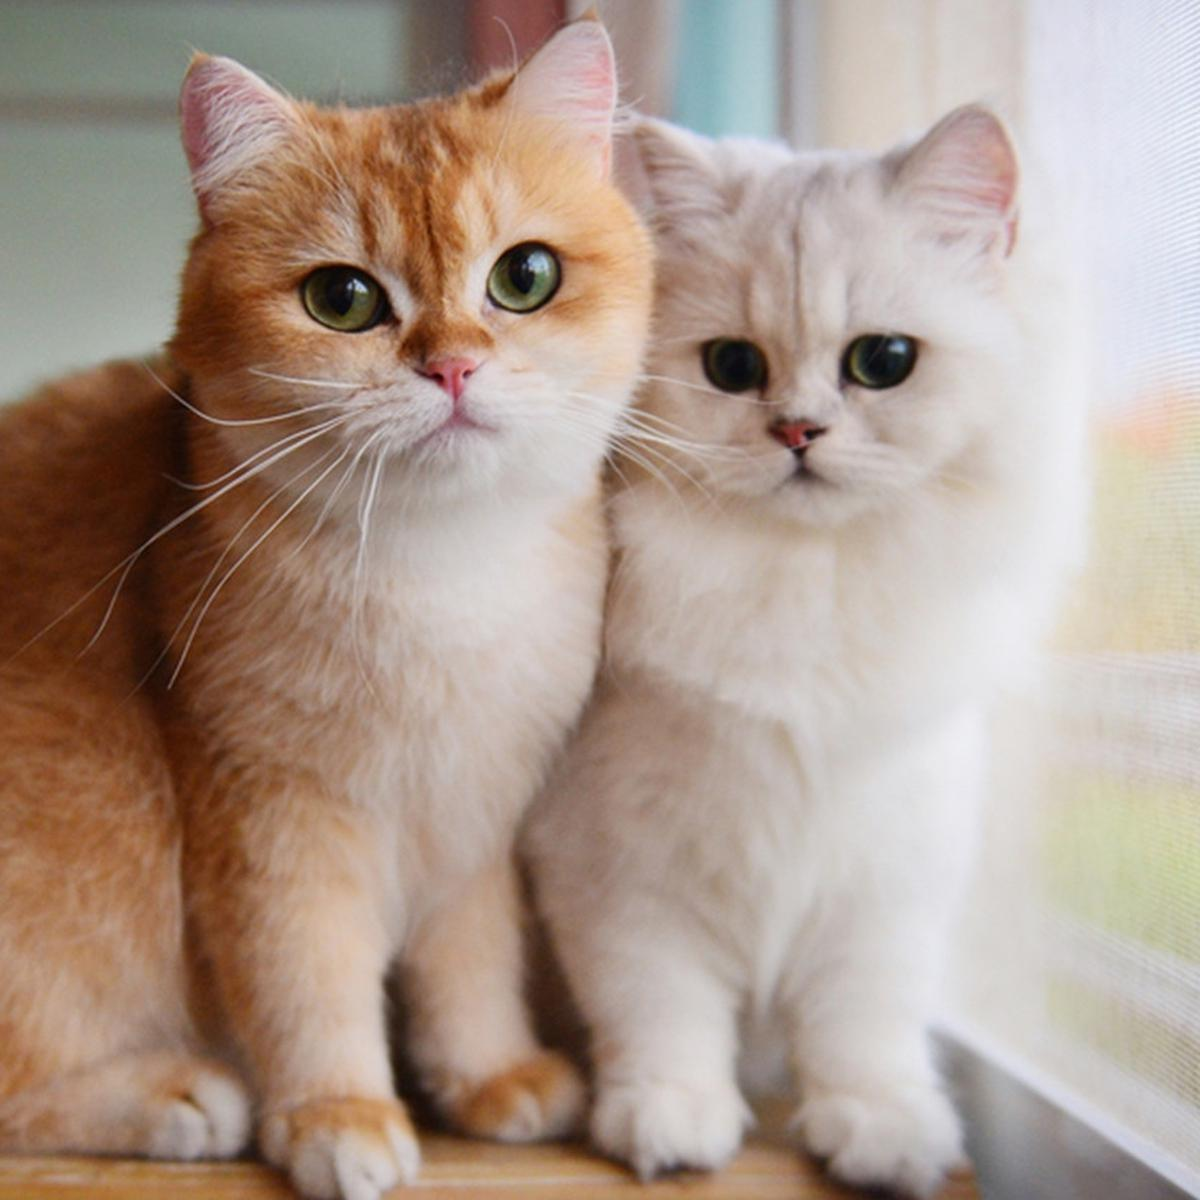
\includegraphics[scale=0.2]{gambar-kucing}
%        \caption{Gambar Kucing Lucu dan Imut}
%    \end{figure}
%\end{lstlisting}

Ukuran gambar dapat diganti dengan mengganti nilai pada scale. Jangan lupa memberikan caption pada setiap gambar. Berikut adalah contoh dari gambar yang telah dimasukkan pada dokumen. Penomoran gambar sudah otomatis dan akan masuk ke daftar gambar juga secara otomatis. Apabila ada beberapa gambar yang akan di embed dengan 1 caption, maka silahkan edit terlebih dahulu dan dijadikan menjadi 1 gambar. Posisi gambar akan pasti setelah dari text ini, apabila ingin mengganti posisinya parameter \textit{H} dapat diganti dengan \textit{h, t, b, p} sesuai kebutuhan.

\begin{figure}[H]
    \centering
    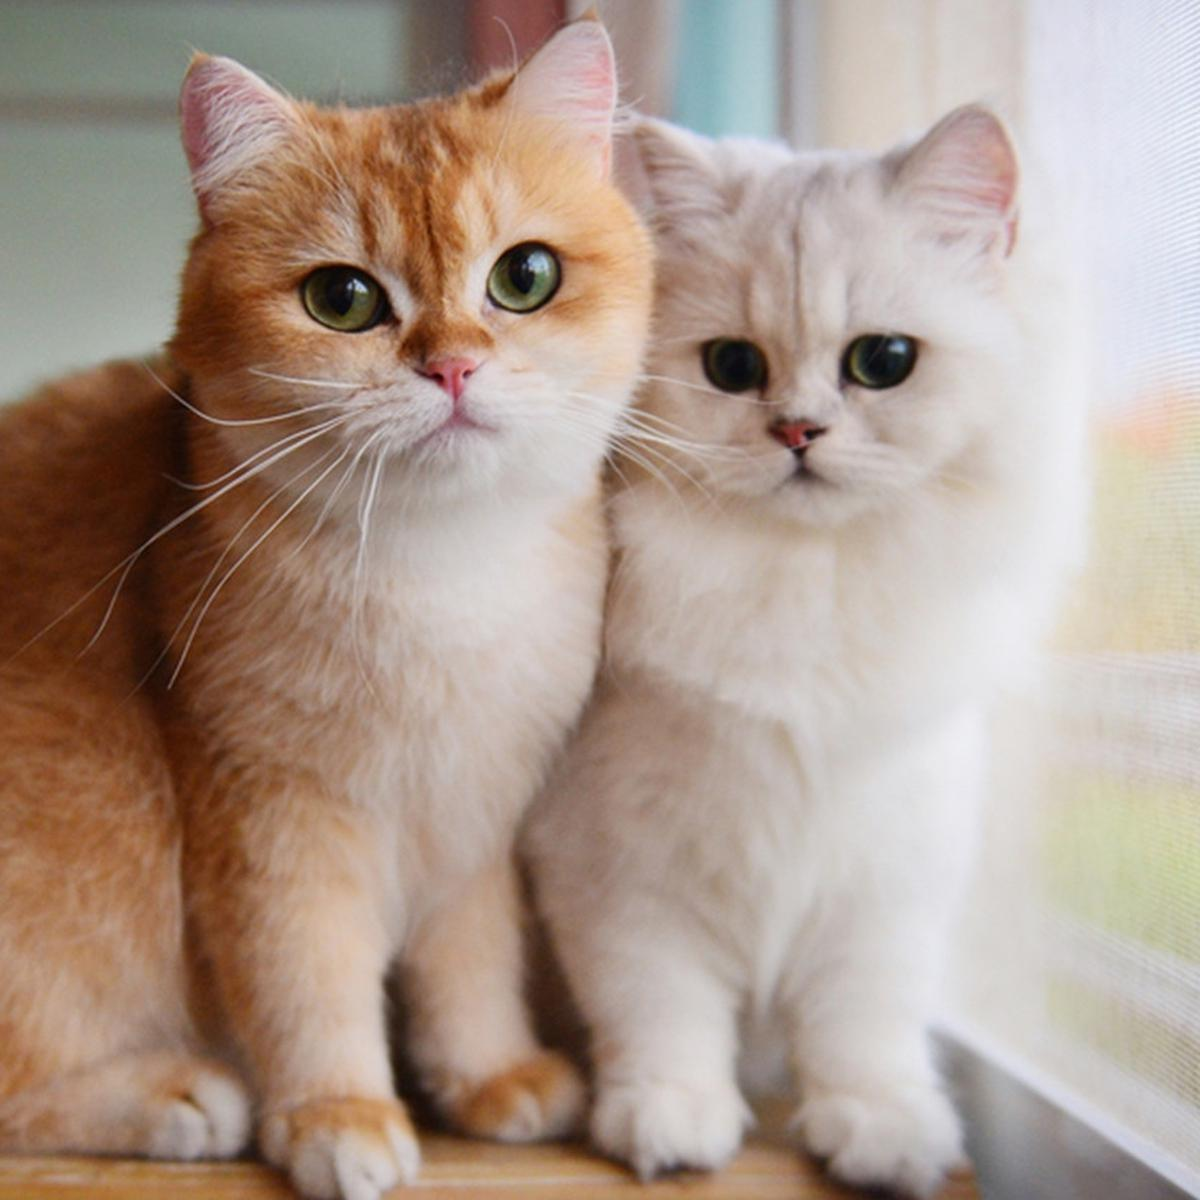
\includegraphics[scale=0.1]{gambar-kucing}
    \caption{Gambar Kucing Lucu dan Imut dengan scala 0.1}
    \label{fig:kucing}
\end{figure}

Setiap gambar harus dimention atau disebutkan didalam bacaan seperti berikut ini \cref{fig:kucing}.

\begin{figure}[H]
    \centering
    
\includegraphics[scale=0.4]{logo-uny}
    \caption{Logo UNY dengan scala 0.4}
    \label{fig:logoUNY}
\end{figure}

Untuk menambahkan gambar secara landscape dapat dilihat pada contoh berikut ini dan jangan lupa selalu menyebutkan nomor gambar disertai penjelasannya seperti ini \cref{fig:logoUNY}.

\begin{sidewaysfigure}[htbp]
	\centering
	
\includegraphics[width=0.6\textwidth]{logo-uny}
	\caption{Logo UNY pada Landscape mode}
    \label{fig:logoUNYlandscape}
\end{sidewaysfigure}

\begin{figure}[H]
    \centering
    \subfigure[]{
     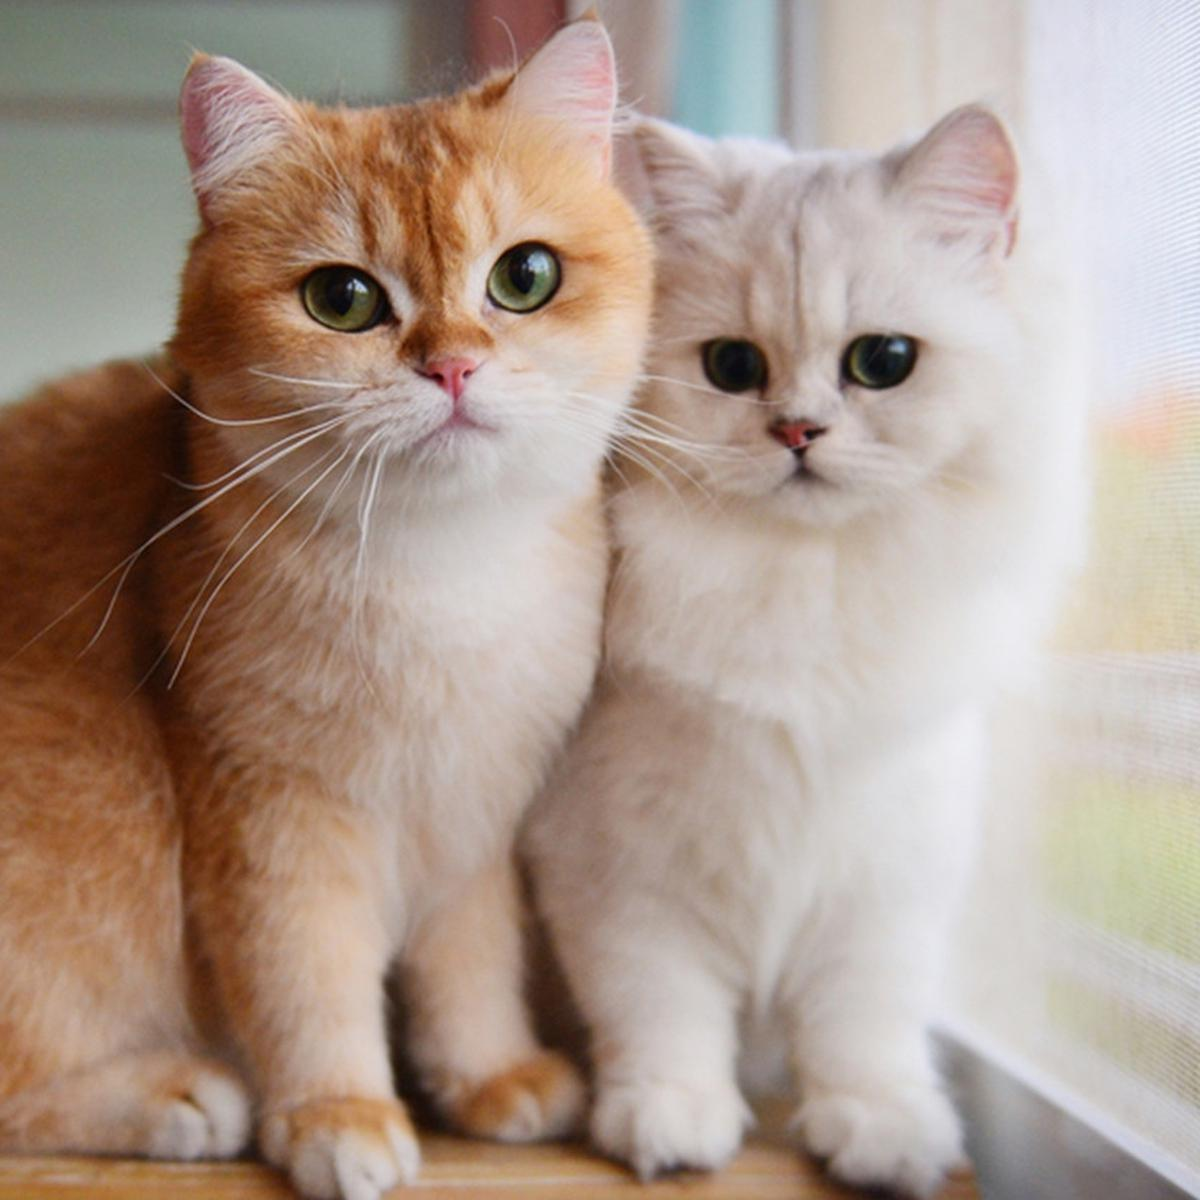
\includegraphics[width=0.4\linewidth]{gambar-kucing}
     }\hspace{0.1\linewidth}
    \subfigure[]{
     
\includegraphics[width=0.4\linewidth]{logo-uny}
    }
    \caption{Dengan menempatkan gambar (a) dan (b), pembaca akan lebih mudah membandingkan keduanya.}
    \label{fig:kucingdanUNY}
\end{figure}

\subsection{Membuat Tabel}
Pada bagian ini akan dijelaskan bagaimana membuat tabel dalam sebuah dokumen \LaTeX. untuk membuat tabel memang agak sedikit sulit, sehingga saya menyarankan menggunakan tool berikut \url{https://www.tablesgenerator.com/} kemudian isikan tabel pada tool generator tersebut dan salin kodenya ke dalam dokumen \LaTeX. Berikut adalah contoh dari sebuah tabel yang telah dibuat. Jangan lupa setiap tabel harus dimention dan dijelaskan dibacaan seperti berikut ini \cref{tab:spekPC}.


\begin{longtable}{|p{2cm}|p{7cm}|}
    \caption{Spesifikasi komputer untuk menjalankan simulator.}
    \label{tab:spekPC} \\
    \hline
    OS     & Ubuntu 20.04.2 LTS             \\ \hline
    Kernel & 5.4.0-80-generic               \\ \hline
    CPU    & Intel i3-8100 (4) @ 3.600GH    \\ \hline
    GPU    & NVIDIA GeForce GTX 1050 Ti     \\ \hline
    RAM    & 7901 MiB                       \\ \hline
\end{longtable}

Kita juga bisa menambahkan tabel yang besar dengan format halaman landscape seperti contoh berikut dan mention tabel seperti berikut ini \cref{tab:landscape} dan berikut ini \cref{tab:tabelx}.
\begin{sidewaysfigure}[htbp]
	\begin{table}[H]
		\caption{Tabel Sederhana}
		\label{tab:landscape}
		\begin{center}
			\begin{tabularx}{0.8\textwidth} {
					|>{\raggedright\arraybackslash}X
					|>{\raggedright\arraybackslash}X
					|>{\raggedright\arraybackslash}X
					|}
				\hline
				$G$     & $\text{dim }G$      & $\text{dim }F$ \\
				\hline
				$SU(N)$ & $N^2 -1$            & $N$            \\
				$SO(N)$ & $\frac{1}{2}N(N-1)$ & $N$            \\
				$Sp(N)$ & $N(2N+1)$           & $2N$           \\
				$E_6$   & $78$                & $27$           \\
				$E_7$   & $133$               & $56$           \\
				$E_8$   & $248$               & $248$          \\
				$F_4$   & $52$                & $6$            \\
				$G_2$   & $14$                & $7$            \\
				\hline
			\end{tabularx}
		\end{center}
	\end{table}
\end{sidewaysfigure}

\begin{table}[H]
	\caption{Tabel Sederhana}
	\label{tab:tabelx}
	\begin{center}
		\begin{tabularx}{0.8\textwidth} {
				|>{\raggedright\arraybackslash}X
				|>{\raggedright\arraybackslash}X
				|>{\raggedright\arraybackslash}X
				|}
			\hline
			$G$     & $\text{dim }G$      & $\text{dim }F$ \\
			\hline
			$SU(N)$ & $N^2 -1$            & $N$            \\
			$SO(N)$ & $\frac{1}{2}N(N-1)$ & $N$            \\
			$Sp(N)$ & $N(2N+1)$           & $2N$           \\
			$E_6$   & $78$                & $27$           \\
			$E_7$   & $133$               & $56$           \\
			$E_8$   & $248$               & $248$          \\
			$F_4$   & $52$                & $6$            \\
			$G_2$   & $14$                & $7$            \\
			\hline
		\end{tabularx}
	\end{center}
\end{table}

\subsection{Menambahkan listing Kode Program}
Berikut adalah beberapa contoh listing kode yang diembed ke dalam dokumen \LaTeX. kita bisa menentukan bahasa pemrograman yang digunakan, misal seperti python. Berikut adalah contoh dari kode java, python, octave, dan C. Selain itu juga banyak paket yang bisa digunakan untuk styling / highlighting sumber kode yang digunakan, apabila dirasa dibutuhkan bisa ditambahkan manual.

\lstinputlisting[caption=Contoh Kode Program Python, label={lst:listing-python}, language=Python]{kode/code_sample.py}

\lstinputlisting[caption=Contoh Kode Program C++, label={lst:listing-cpp}, language=C++]{kode/code_sample.cpp}

\lstinputlisting[caption=Contoh Kode Program Arduino, label={lst:listing-cpp}, language=C++]{kode/code_sample.ino}

\lstinputlisting[caption=Contoh Kode Program Java, label={lst:listing-java}, language=C++]{kode/code_sample.java}


\subsection{Menambahkan Persamaan}
Persamaan tidak lepas dari bidang ilmu teknik dan kadang perlu dituliskan dalam sebuah laporan. Sangat mudah menuliskan persamaan pada sebuah dokumen \LaTeX. Terdapat 2 jenis penulisan persamaan, yaitu inline dengan text seperti contoh ini \(x^2 + y^2 = z^2\) atau seperti ini $E=mc^2$. Jenis lain adalah dituliskan seperti dibawah ini, yang otomatis akan mendapatkan penomoran. Apabila belum familiar dengan kode untuk penulisan persamaan pada \LaTeX bisa menggunakan tool berikut \url{https://latex.codecogs.com/eqneditor/editor.php}. Setiap persamaan harus dimention seperti berikut ini \cref{eq:satu} dan harus dijelaskan terkait persamaan tersebut untuk apa.

\begin{equation}
    \label{eq:satu}
    E=mc^2
\end{equation}

\subsection{Referensi dan Sitasi}
Referensi dan sitasi pada dokumen \LaTeX juga cukup mudah. Silahkan buka file \textit{pustaka.bib} dan amati beberapa contoh penulisan referensi yang ada. Untuk menggenerate bentuk referensi seperti ini dapat menggunakan Mendeley atau Zotero. Mensitasi referensi seperti ini \cite{Kim2006} dapat dilakukan dengan perintah \verb|\cite{nama_label}|.

\section{Section 3.3}
Desain dan Implementasi

\subsection{Subsection 3.3.1}
Bagian ini digunakan apabila dibutuhkan, silahkan bisa ditambah atau dikurangi sesuai kebutuhan.

\subsection{Subsection 3.3.2}
Bagian ini digunakan apabila dibutuhkan, silahkan bisa ditambah atau dikurangi sesuai kebutuhan.

\subsection{Subsection 3.3.3}
Bagian ini digunakan apabila dibutuhkan, silahkan bisa ditambah atau dikurangi sesuai kebutuhan.

\section{Section 3.4}
Desain dan Implementasi

\subsection{Subsection 3.4.1}
Bagian ini digunakan apabila dibutuhkan, silahkan bisa ditambah atau dikurangi sesuai kebutuhan.

\subsection{Subsection 3.4.2}
Bagian ini digunakan apabila dibutuhkan, silahkan bisa ditambah atau dikurangi sesuai kebutuhan.

\subsection{Subsection 3.4.3}
Bagian ini digunakan apabila dibutuhkan, silahkan bisa ditambah atau dikurangi sesuai kebutuhan.

\section{Section 3.5}
Section maupun subsection dapat ditambah atau dikurangi sesuai dengan kebutuhan.

\subsection{Subsection 3.5.1}
Bagian ini digunakan apabila dibutuhkan, silahkan bisa ditambah atau dikurangi sesuai kebutuhan.

\subsection{Subsection 3.5.2}
Bagian ini digunakan apabila dibutuhkan, silahkan bisa ditambah atau dikurangi sesuai kebutuhan.

\subsection{Subsection 3.5.3}
Bagian ini digunakan apabila dibutuhkan, silahkan bisa ditambah atau dikurangi sesuai kebutuhan.
		\chapter[Penulisan dengan \LaTeX - INI HANYA TUTORIAL]{\\ Penulisan dengan \LaTeX  - INI HANYA TUTORIAL}

\section{Membuat List atau Daftar}
Terdapat 2 cara yaitu dengan list yang terdapat penomoran 1,2,3 dst atau dengan bullet poin. Secara detail dapat dibaca pada subsection di bawah.
\subsection{List atau Daftar dengan \texttt{packed\_enum}}
Lingkungan \texttt{packed\_enum} digunakan untuk membuat daftar bernomor dengan jarak yang lebih rapat antar item. Ini sangat berguna untuk menampilkan langkah atau tahapan yang memiliki urutan. Berikut adalah contoh penggunaannya:

\begin{lstlisting}
    \begin{packed_enum}
        \item Langkah pertama adalah mengidentifikasi masalah yang ingin diselesaikan.
        \item Langkah kedua melibatkan analisis kebutuhan.
        \item Langkah ketiga adalah mengembangkan ide dan solusi alternatif.
        \item Langkah keempat adalah melakukan pengujian awal untuk mengevaluasi performa.
    \end{packed_enum}
\end{lstlisting}
    
Hasilnya akan tampak seperti berikut:
\begin{packed_enum}
    \item Langkah pertama adalah mengidentifikasi masalah yang ingin diselesaikan.
    \item Langkah kedua melibatkan analisis kebutuhan.
    \item Langkah ketiga adalah mengembangkan ide dan solusi alternatif.
    \item Langkah keempat adalah melakukan pengujian awal untuk mengevaluasi performa.
\end{packed_enum}

\subsection{List atau Daftar dengan \texttt{packed\_item}}
Lingkungan \texttt{packed\_item} digunakan untuk membuat daftar berpoin dengan jarak antar item yang lebih rapat, cocok untuk poin-poin yang tidak memerlukan urutan tertentu. Berikut adalah contoh penggunaannya:

\begin{lstlisting}
    \begin{packed_item}
        \item Meningkatkan kualitas sensor untuk akurasi yang lebih baik.
        \item Menambahkan modul komunikasi untuk kontrol jarak jauh.
        \item Mengoptimalkan kode untuk efisiensi.
        \item Menambah fitur penghematan energi.
    \end{packed_item}
\end{lstlisting}

Hasilnya akan tampak seperti berikut:
\begin{packed_item}
    \item Meningkatkan kualitas sensor untuk akurasi yang lebih baik.
    \item Menambahkan modul komunikasi untuk kontrol jarak jauh.
    \item Mengoptimalkan kode untuk efisiensi.
    \item Menambah fitur penghematan energi.
\end{packed_item}

\section{Menuliskan Kode Program dengan Listing}
Lingkungan \texttt{lstlisting} memungkinkan kita untuk menuliskan atau menyisipkan kode Python, C++, Arduino, Java atau lainnya dalam dokumen LaTeX dengan format yang rapi dan terstruktur. Pada bagian ini, kita akan melihat dua cara untuk menuliskan kode Python: secara langsung di dalam dokumen dan dengan mengambil dari file eksternal.

\Cref{lst:python_direct} menunjukkan fungsi Python yang menghitung faktorial dari sebuah angka. Kode ini ditulis langsung di dalam dokumen LaTeX menggunakan lingkungan \texttt{lstlisting} dengan format diawali dengan \texttt{\textbackslash begin\{lstlisting\}[language=Python, caption=Contoh Kode Python Langsung, label=lst:python\_direct]} dan diakhiri dengan \texttt{\textbackslash end\{lstlisting\}}, dimana:
\begin{packed_item}
    \item \texttt{language=Python}: Mengatur pewarnaan sintaksis untuk Python.
    \item \texttt{caption}: Menambahkan keterangan di atas kode untuk menjelaskan isi kode.
    \item \texttt{label}: Menambahkan label untuk memudahkan referensi kode dalam dokumen.
\end{packed_item}

\begin{lstlisting}[language=Python, caption=Contoh Kode Python Langsung, label=lst:python_direct]
    def factorial(n):
        if n == 0:
            return 1
        else:
            return n * factorial(n-1)
\end{lstlisting}

Jika Anda memiliki file kode Python di folder tertentu (misalnya, di \texttt{kode/code\_sample.py}), Anda bisa menyisipkan kode tersebut langsung ke dalam dokumen LaTeX menggunakan perintah \texttt{\textbackslash lstinputlisting}. Berikut \cref{lst:python_file} dengan format penulisan \texttt{\textbackslash lstinputlisting[language=Python, caption=Contoh Kode Python dari File, label=lst:python\_file]\{kode/code\_sample.py\}}, dimana:
\begin{packed_item}
    \item \texttt{language=Python}: Mengatur pewarnaan sintaksis untuk Python.
    \item \texttt{caption}: Menambahkan keterangan untuk kode yang diambil dari file.
    \item \texttt{label}: Menambahkan label untuk referensi.
    \item \texttt{\{kode/code\_sample.py\}}: Menentukan path atau lokasi file Python yang akan disisipkan. Pastikan file berada di dalam folder \texttt{kode} atau path yang sesuai.
\end{packed_item}

\lstinputlisting[language=Python, caption=Contoh Kode Python dari File, label=lst:python_file]{kode/code_sample.py}

\section{Menambahkan Gambar}
Untuk menambahkan gambar hal yang harus dilakukan adalah:
\begin{packed_enum}
    \item Menyalin file gambar (dalam format jpg \/ png) ke dalam folder \textit{gambar}
    \item Mengganti nama file dari gambar agar mudah dikenali, jangan diberi nama gambar-1,-2, dst
    \item Memasukkan seperti \cref{lst:kode_gambar}
\end{packed_enum}

\begin{lstlisting}[language=TeX, caption=Kode untuk Menyisipkan Gambar dalam Dokumen, label=lst:kode_gambar]
    \begin{figure}[H]
        \centering
        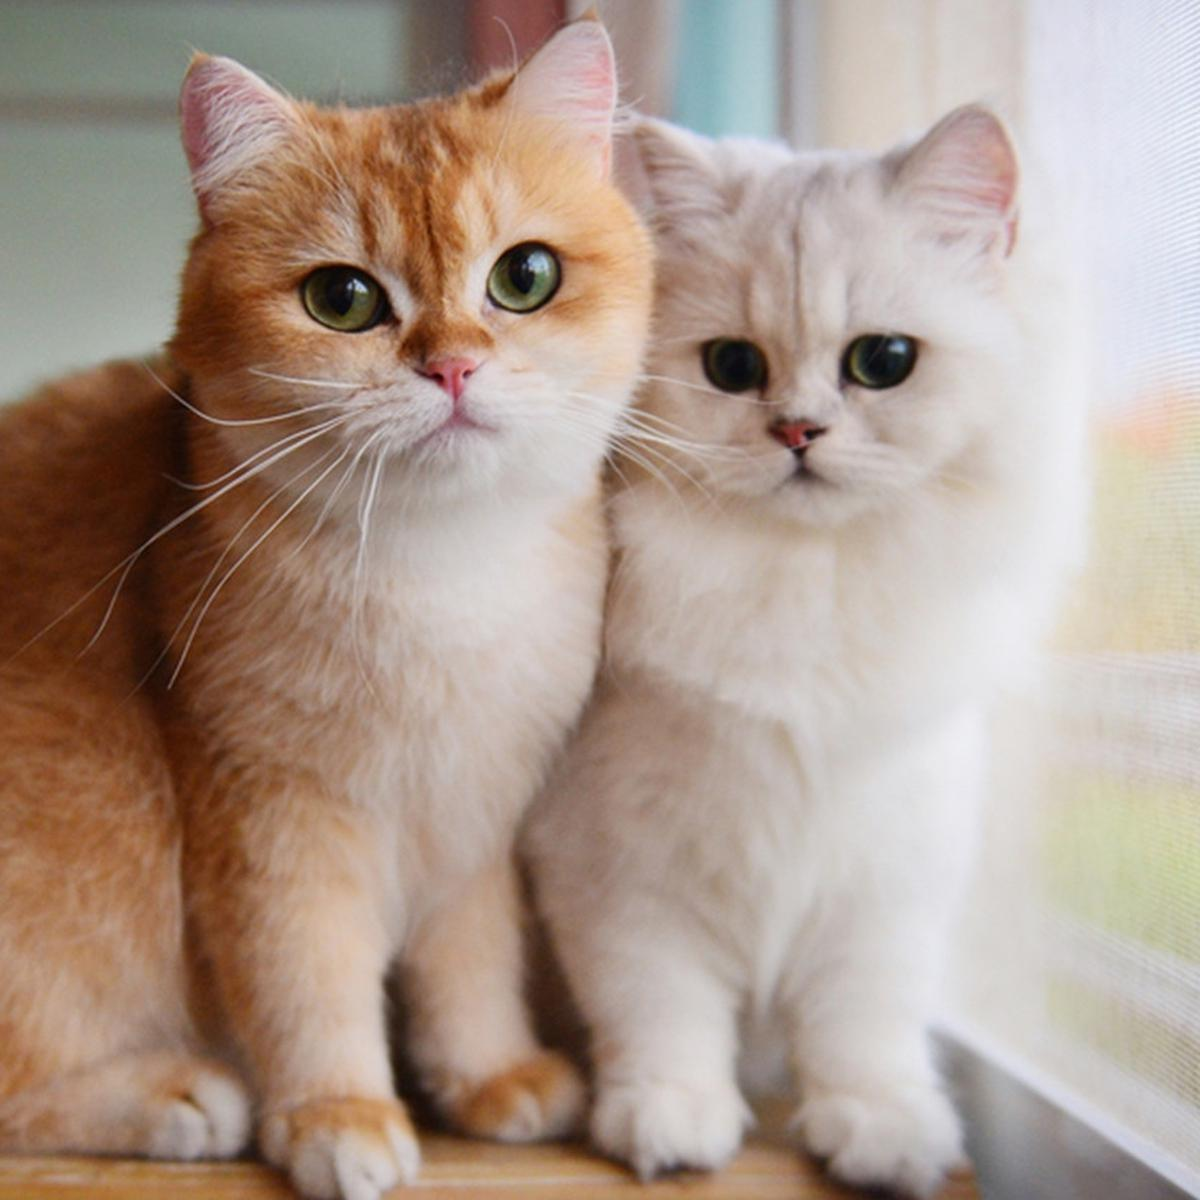
\includegraphics[scale=0.2]{gambar-kucing.jpg}
        \caption{Gambar Kucing Lucu dan Imut}
        \label{fig:kucing}
    \end{figure}
\end{lstlisting}

\noindent Berikut adalah penjelasan dari setiap baris pada kode di atas:

\begin{packed_enum}
    \item \texttt{\textbackslash begin\{figure\}[H] ... \textbackslash end\{figure\}}: Membuat lingkungan \texttt{figure} untuk menyisipkan gambar. Parameter \texttt{[H]} digunakan agar gambar diletakkan tepat di posisi yang ditentukan dalam kode. Opsi \textit{H} dapat diganti dengan \textit{h, t, b, p} sesuai kebutuhan.
    \item \texttt{\textbackslash centering}: Mengatur gambar agar berada di tengah halaman.
    \item \texttt{\textbackslash includegraphics[scale=0.2]\{gambar-kucing.jpg\}}: Memasukkan gambar dengan nama file \texttt{gambar-kucing.jpg}. Parameter \texttt{scale=0.2} mengatur ukuran gambar pada 20\% dari ukuran aslinya. Ubah nilainya untuk memperbesar atau memperkecil gambar.
    \item \texttt{\textbackslash caption\{Gambar Kucing Lucu dan Imut\}}: Menambahkan keterangan (caption) di bawah gambar yang akan muncul di Daftar Gambar dan disertai nomor gambar secara otomatis.
    \item \texttt{\textbackslash label\{fig:kucing\}}: Memberikan label pada gambar untuk merujuk gambar ini dalam teks menggunakan \texttt{\textbackslash cref\{fig:kucing\}} atau \texttt{\textbackslash ref\{fig:kucing\}} yang menghasilkan "Gambar 1" atau penomoran gambar sesuai urutan.
\end{packed_enum}

Hasilnya adalah terlihat seperti pada \cref{fig:kucing}.

\begin{figure}[H]
    \centering
    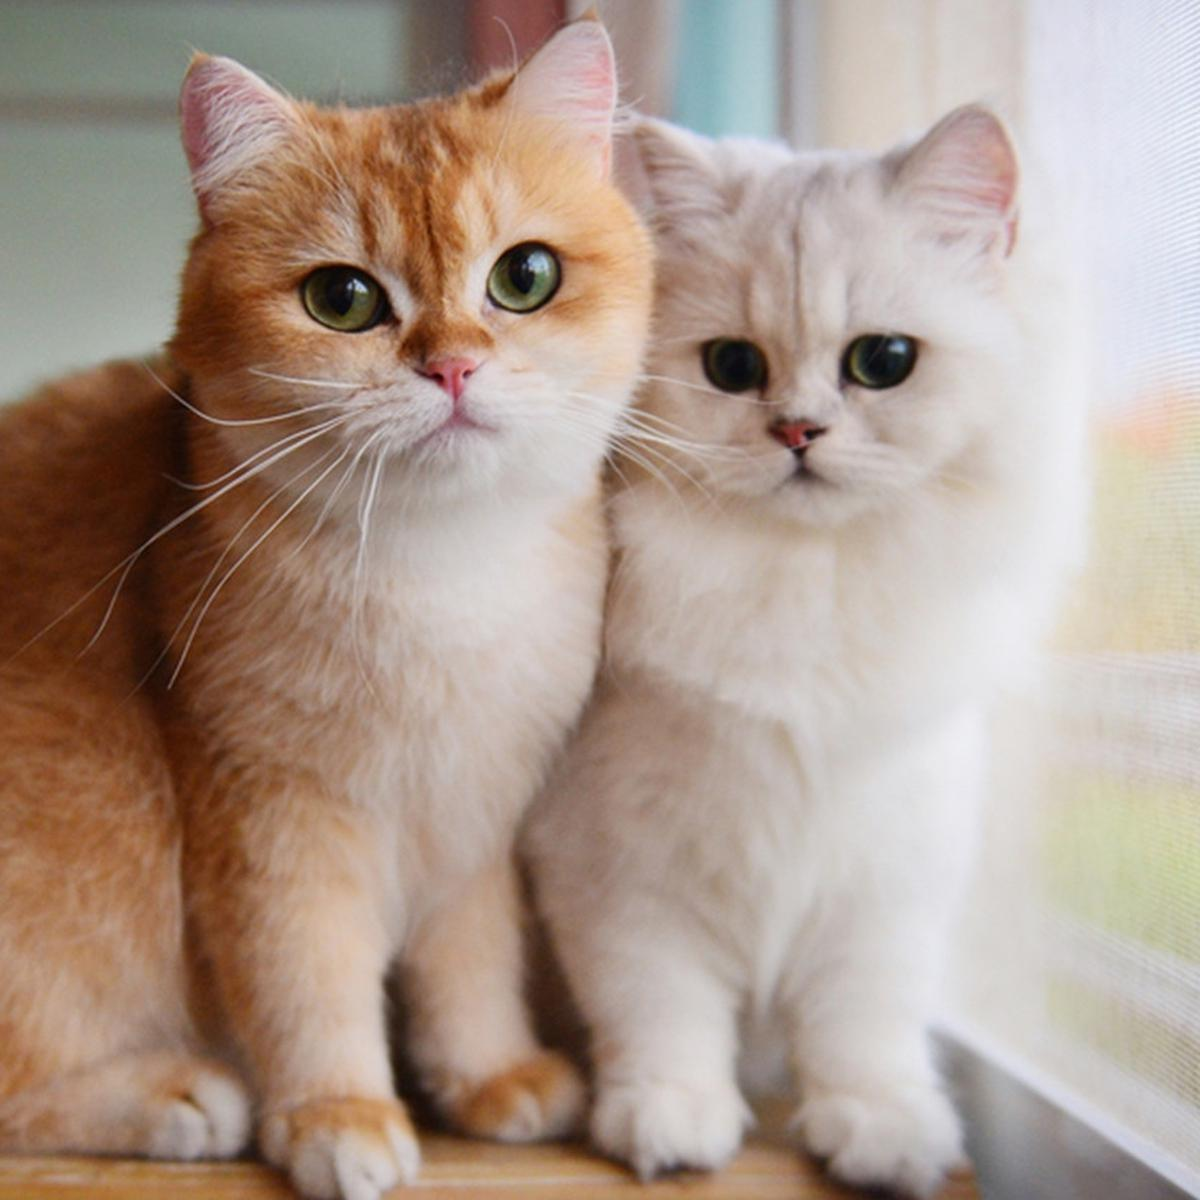
\includegraphics[scale=0.1]{gambar-kucing}
    \caption{Gambar Kucing Lucu dan Imut dengan scala 0.1}
    \label{fig:kucing}
\end{figure}

Setiap gambar harus dimention atau disebutkan didalam bacaan seperti berikut ini \cref{fig:kucing} dan \cref{fig:logoUNY}.

\begin{figure}[H]
    \centering
    
\includegraphics[scale=0.4]{logo-uny}
    \caption{Logo UNY dengan scala 0.4}
    \label{fig:logoUNY}
\end{figure}

Untuk menyisipkan beberapa gambar dalam satu kelompok dan satu caption utama, kita dapat menggunakan lingkungan \texttt{subfigure} di dalam lingkungan \texttt{figure}. Metode ini sangat bermanfaat jika kita ingin menyusun beberapa gambar berukuran kecil dalam satu baris atau kolom, dengan setiap gambar diberi caption masing-masing dan satu caption utama untuk keseluruhan gambar.

Kode berikut menunjukkan cara menyusun tiga gambar secara berdampingan dengan satu caption utama.

\begin{lstlisting}[language=TeX, caption=Kode untuk Menyisipkan Gambar dalam Dokumen dengan Subfigure, label=lst:kode_gambar_multi]
    \begin{figure}
        \centering
        \begin{subfigure}[b]{0.3\textwidth}
            \centering
            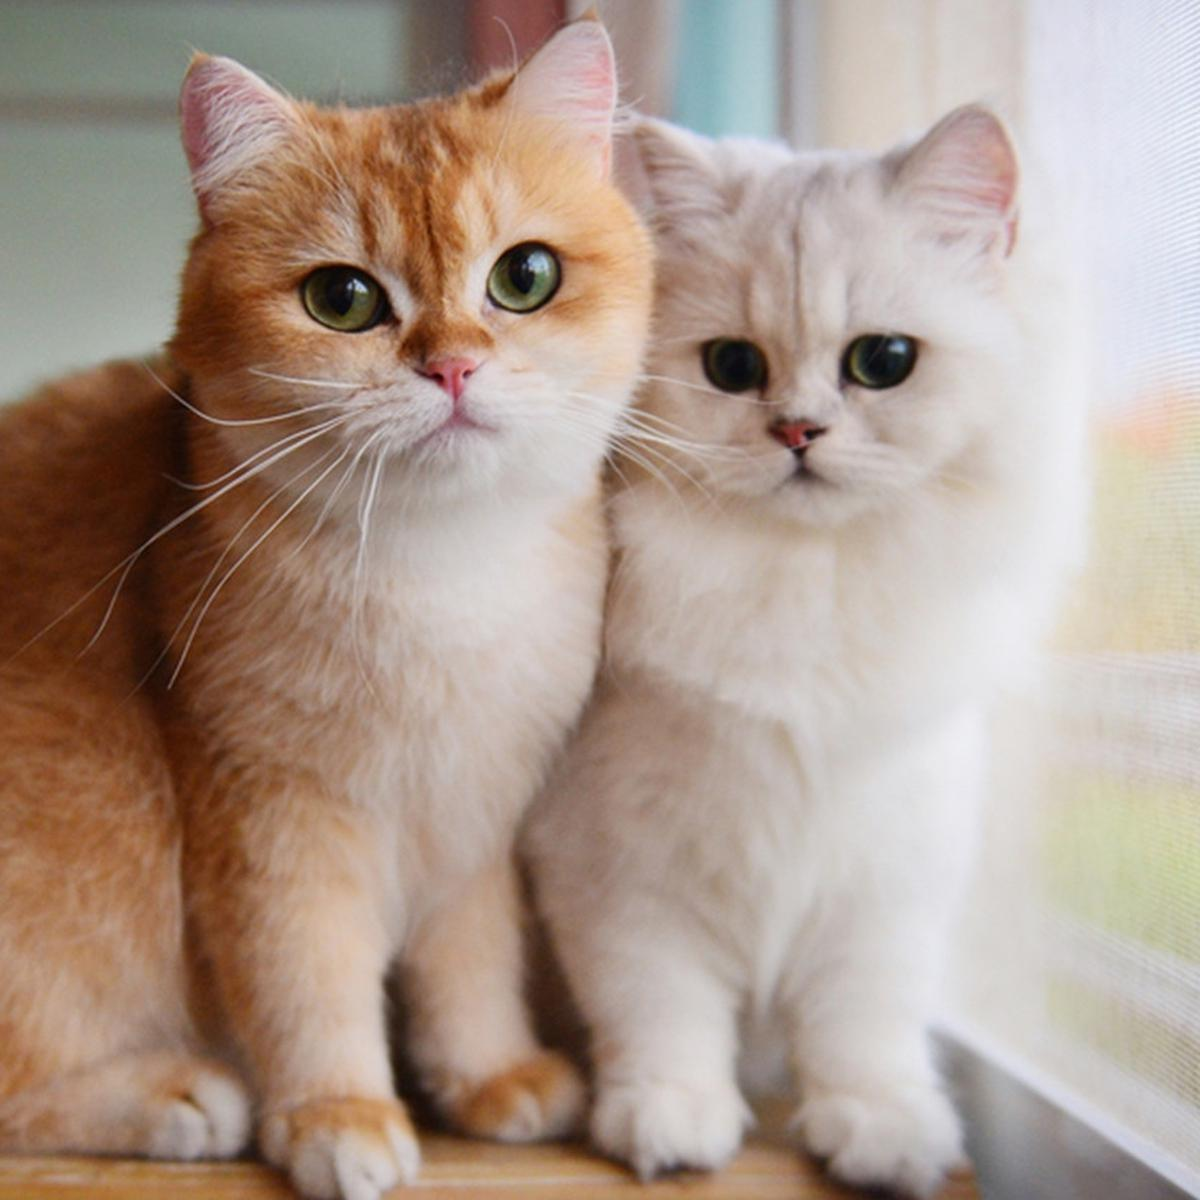
\includegraphics[width=\linewidth]{gambar-kucing.jpg}
            \caption{Kucing Lucu 1}
            \label{fig:kucing-a}
        \end{subfigure}
        \hfill
        \begin{subfigure}[b]{0.3\textwidth}
            \centering
            
\includegraphics[width=\linewidth]{logo-uny.png}
            \caption{Logo UNY}
            \label{fig:logo-uny-b}
        \end{subfigure}
        \hfill
        \begin{subfigure}[b]{0.3\textwidth}
            \centering
            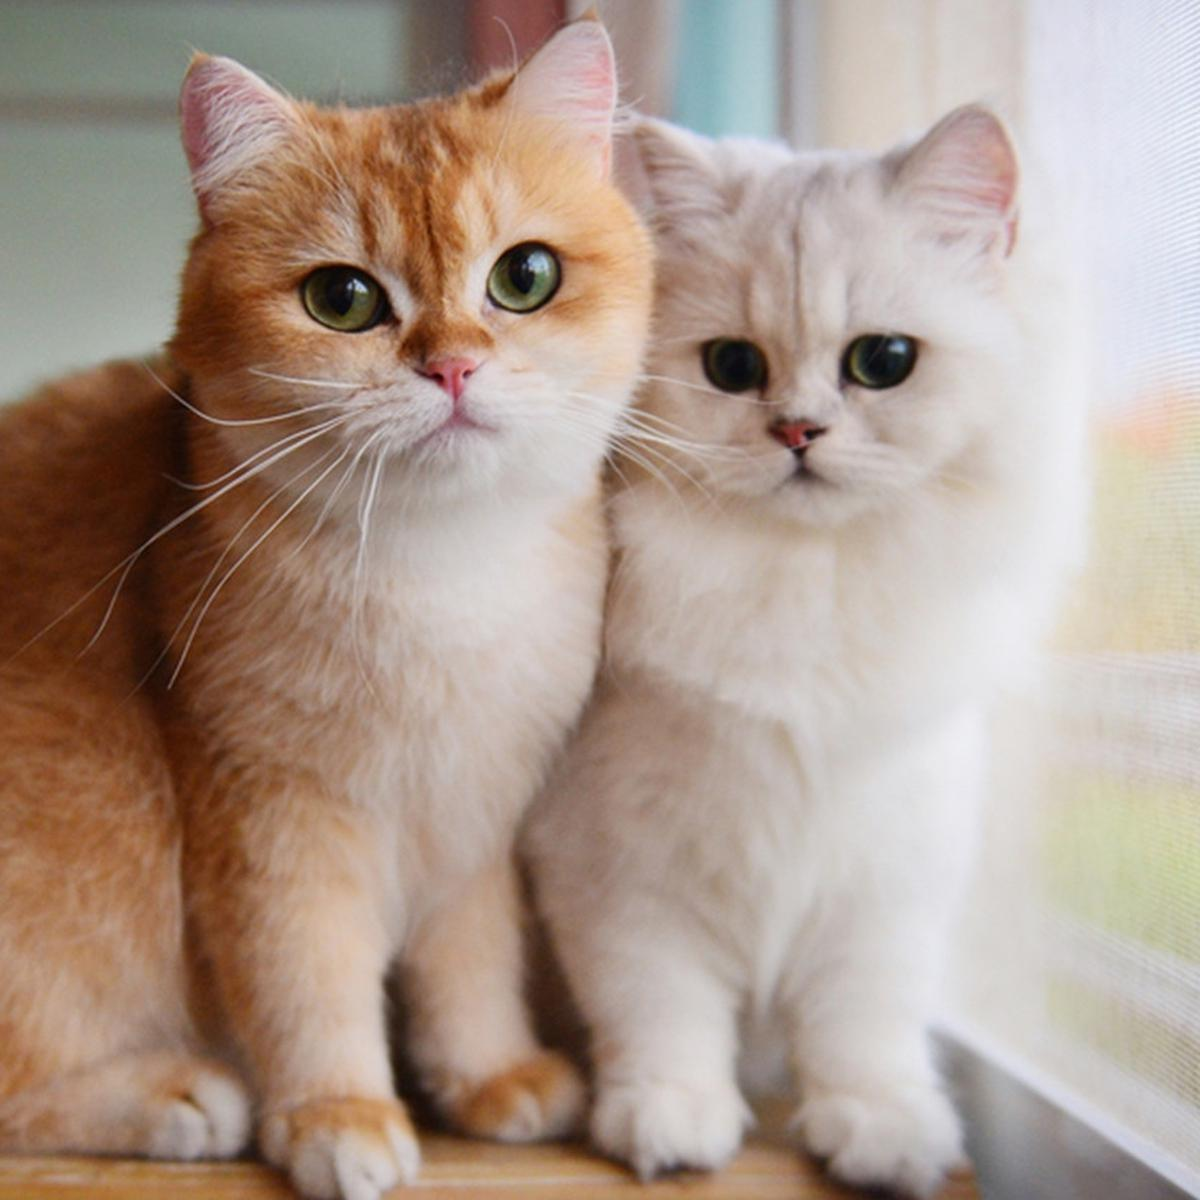
\includegraphics[width=\linewidth]{gambar-kucing.jpg}
            \caption{Kucing Lucu 2}
            \label{fig:kucing-c}
        \end{subfigure}
        \caption{Beberapa gambar yang disusun menjadi 1 bagian dengan penomoran (a), (b), dan (c)}
        \label{fig:kucingdanUNY}
    \end{figure}
\end{lstlisting}

\noindent Berikut adalah penjelasan dari setiap bagian kode di atas:

\begin{packed_enum}
    \item \texttt{\textbackslash begin\{figure\} ... \textbackslash end\{figure\}}: Lingkungan \texttt{figure} utama yang berfungsi sebagai wadah untuk menyisipkan beberapa gambar dalam satu bagian.
    
    \item \texttt{\textbackslash begin\{subfigure\}[b]\{0.3\textbackslash textwidth\} ... \textbackslash end\{subfigure\}}: Lingkungan \texttt{subfigure} digunakan untuk setiap gambar yang ingin disusun dalam satu bagian. Parameter \texttt{0.3\textbackslash textwidth} mengatur lebar setiap gambar menjadi sepertiga dari lebar teks, sehingga tiga gambar dapat ditampilkan berdampingan dalam satu baris.
    
    \item \texttt{\textbackslash includegraphics[width=\textbackslash linewidth]\{gambar-nama\}}: Memasukkan setiap gambar dengan lebar yang sesuai dengan lebar yang telah ditentukan untuk \texttt{subfigure}. 
        \begin{packed_enum}
            \item Gambar pertama menggunakan file \texttt{gambar-kucing}, dengan caption "Kucing Lucu 1".
            \item Gambar kedua menggunakan file \texttt{logo-uny}, dengan caption "Logo UNY".
            \item Gambar ketiga juga menggunakan file \texttt{gambar-kucing}, dengan caption "Kucing Lucu 2".
        \end{packed_enum}
    
    \item \texttt{\textbackslash hfill}: Menyisipkan ruang kosong antar gambar, agar setiap \texttt{subfigure} memiliki jarak yang merata.
    
    \item \texttt{\textbackslash caption\{...\}}: Caption utama yang menjelaskan ketiga gambar sekaligus. Caption ini akan ditampilkan di bawah semua gambar dalam lingkungan \texttt{figure}.

    \item \texttt{\textbackslash label\{fig:kucingdanUNY\}}: Memberikan label untuk keseluruhan kelompok gambar, sehingga kita bisa merujuk ke seluruh bagian gambar ini dalam teks dengan \texttt{\textbackslash cref\{fig:kucingdanUNY\}}.
\end{packed_enum}

Dengan menggunakan metode ini, Anda dapat menyisipkan beberapa gambar dalam satu bagian dengan satu caption utama seperti pada \cref{fig:kucingdanUNY}. Setiap gambar dapat memiliki caption terpisah dan nomor (misalnya, (a), (b), (c)), sehingga rujukan spesifik untuk masing-masing gambar dapat dibuat, seperti \texttt{\textbackslash cref\{fig:kucing-a\}} untuk merujuk ke \cref{fig:kucing-a}.

\begin{figure}
    \centering
    \begin{subfigure}[b]{0.3\textwidth}
        \centering
        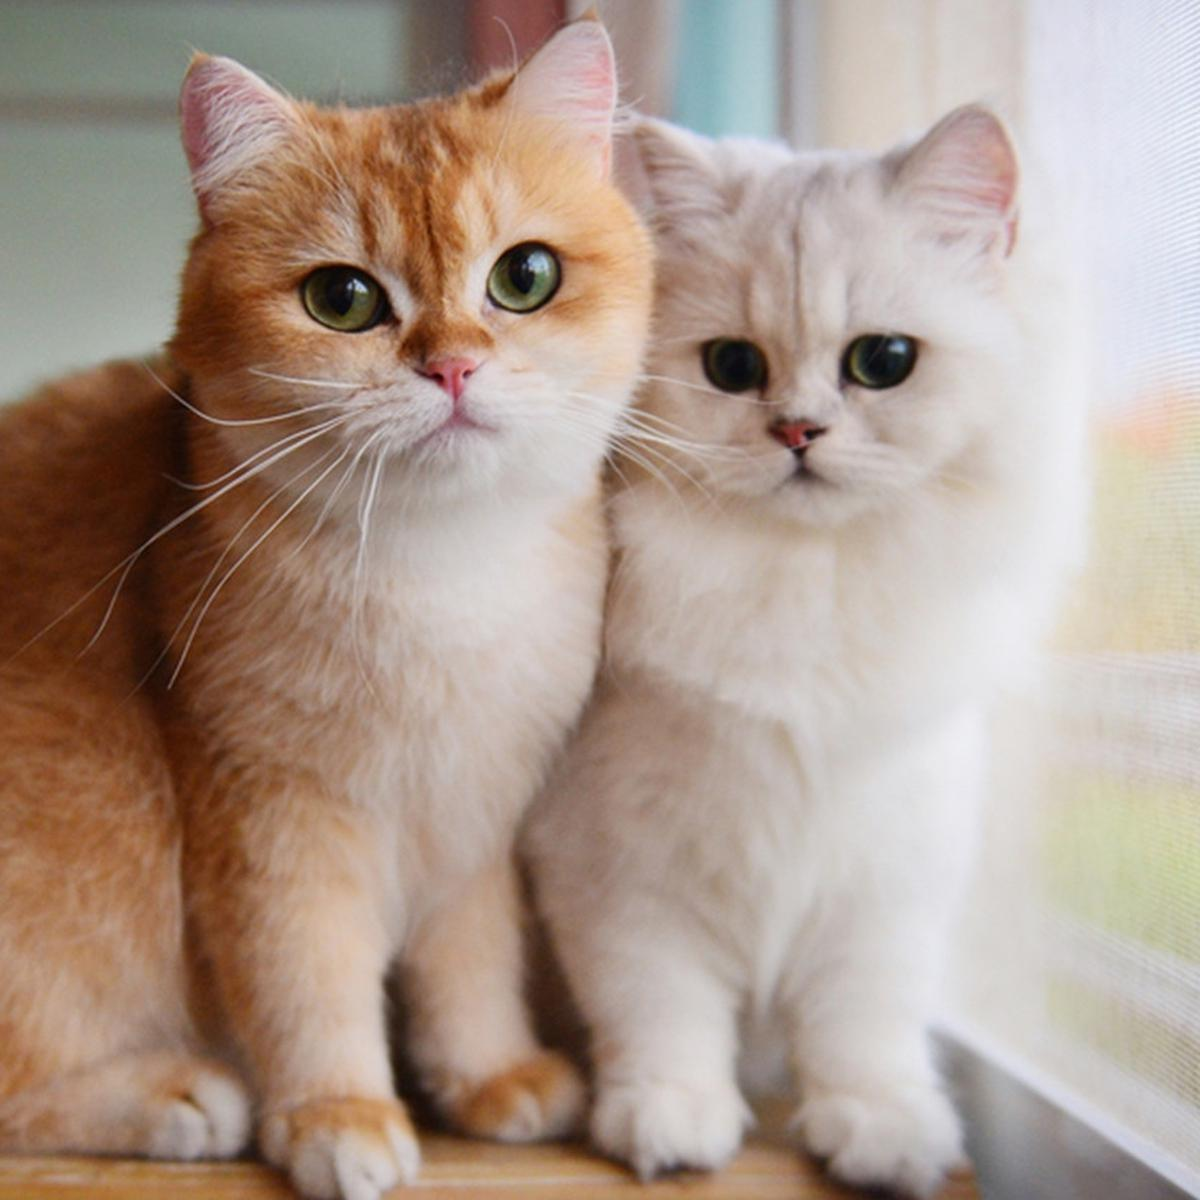
\includegraphics[width=\linewidth]{gambar-kucing.jpg}
        \caption{Kucing Lucu 1}
        \label{fig:kucing-a}
    \end{subfigure}
    \hfill
    \begin{subfigure}[b]{0.3\textwidth}
        \centering
        
\includegraphics[width=\linewidth]{logo-uny.png}
        \caption{Logo UNY}
        \label{fig:logo-uny-b}
    \end{subfigure}
    \hfill
    \begin{subfigure}[b]{0.3\textwidth}
        \centering
        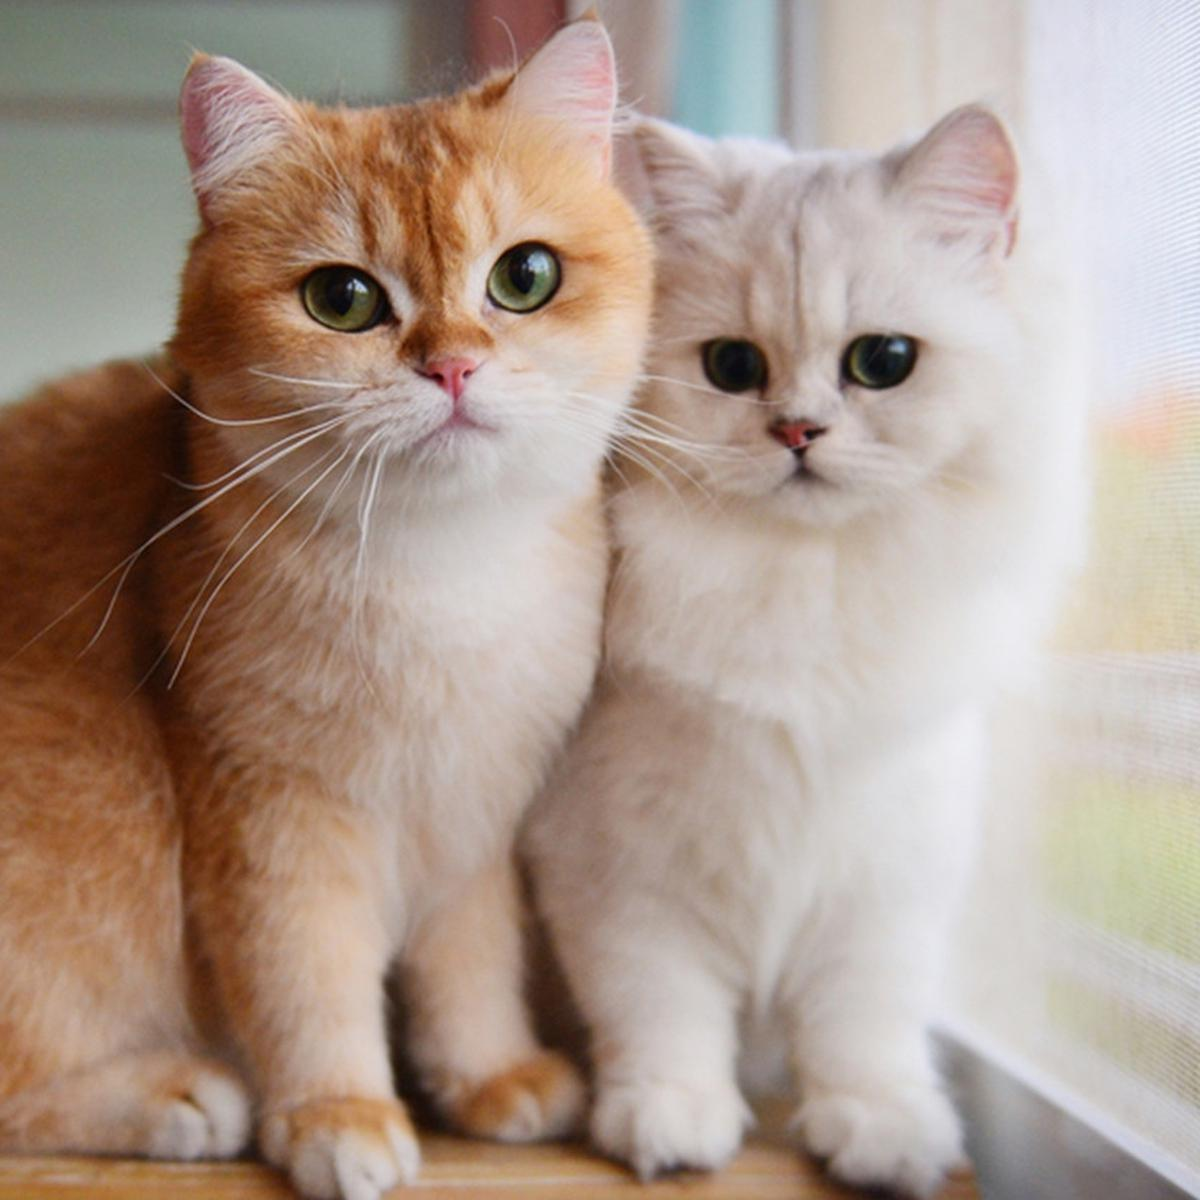
\includegraphics[width=\linewidth]{gambar-kucing.jpg}
        \caption{Kucing Lucu 2}
        \label{fig:kucing-c}
    \end{subfigure}
    \caption{Beberapa gambar yang disusun menjadi 1 bagian dengan penomoran (a), (b), dan (c)}
    \label{fig:kucingdanUNY}
\end{figure}

\section{Membuat Grafik dengan Tikz}
TikZ adalah sebuah paket LaTeX yang digunakan untuk membuat grafik vektor. Berikut adalah beberapa contoh dasar penggunaan TikZ.

\subsection{Menggambar Garis dan Bentuk Dasar}
Untuk menggambar garis dan bentuk dasar, kita bisa menggunakan perintah-perintah berikut:
\begin{lstlisting}[language=TeX, caption=Kode untuk Menggambar Garis dan Bentuk Dasar, label=lst:Menggambar Garis dan Bentuk Dasar]
    \begin{figure}[H]
        \centering
        \begin{tikzpicture}
            \draw (0,0) -- (2,0);
            \draw (0,0) rectangle (2,2);
            \draw (1,1) circle (1);
        \end{tikzpicture}
        \caption{Menggambar Garis dan Bentuk Dasar}
        \label{fig:tikzExample}
    \end{figure}
\end{lstlisting}

\begin{figure}[H]
    \centering
    \begin{tikzpicture}
        \draw (0,0) -- (2,0);
        \draw (0,0) rectangle (2,2);
        \draw (1,1) circle (1);
    \end{tikzpicture}
    \caption{Menggambar Garis dan Bentuk Dasar}
    \label{fig:tikzExample}
\end{figure}

Pada Gambar \ref{fig:tikzExample} dapat dilihat contoh gambar sederhana.

\subsection{Menggambar Grafik Fungsi}
TikZ juga bisa digunakan untuk menggambar grafik fungsi matematika:
\begin{lstlisting}[language=TeX, caption=Kode untuk Menggambar Grafik Fungsi, label=lst:Menggambar Grafik Fungsi]
    \begin{figure}[H]
        \centering
        \begin{tikzpicture}
            \begin{axis}[
                axis lines = middle,
                xlabel = $x$,
                ylabel = {$f(x)$},
                title = {Grafik Fungsi Kuadrat},
                grid = major,
                xmin = -10, 
                xmax = 10,
                ymin = 0, 
                ymax = 100
            ]
            \addplot [
                domain=-10:10, 
                samples=100, 
                color=blue,
            ]
            {x^2};
            \end{axis}
        \end{tikzpicture}
        \caption{Grafik fungsi \( f(x) = x^2 \) dengan domain \( [-10, 10] \)}
        \label{fig:grafik_kuadrat}
    \end{figure}
\end{lstlisting}

\begin{figure}[H]
    \centering
    \begin{tikzpicture}
        \begin{axis}[
            axis lines = middle,
            xlabel = $x$,
            ylabel = {$f(x)$},
            title = {Grafik Fungsi Kuadrat},
            grid = major,
            xmin = -10, 
            xmax = 10,
            ymin = 0, 
            ymax = 100
        ]
        \addplot [
            domain=-10:10, 
            samples=100, 
            color=blue,
        ]
        {x^2};
        \end{axis}
    \end{tikzpicture}
    \caption{Grafik fungsi \( f(x) = x^2 \) dengan domain \( [-10, 10] \)}
    \label{fig:grafik_kuadrat}
\end{figure}

Pada Gambar \ref{fig:grafik_kuadrat} ditunjukkan grafik fungsi kuadrat.

\subsection{Menggambar Diagram Alir}
TikZ juga mendukung pembuatan diagram alir (flowchart):
\begin{lstlisting}[language=TeX, caption=Kode untuk Menggambar Diagram Alir, label=lst:Menggambar Diagram Alir]
    \begin{figure}[H]
        \centering
        \begin{tikzpicture}[node distance=2cm]
            \node (start) [startstop] {Start};
            \node (process1) [process, below of=start] {Process 1};
            \node (decision) [decision, below of=process1] {Decision};
            \node (process2a) [process, below of=decision, yshift=-1cm] {Process 2a};
            \node (process2b) [process, right of=decision, xshift=2cm] {Process 2b};
            \node (stop) [startstop, below of=process2a] {Stop};
    
            \draw [arrow] (start) -- (process1);
            \draw [arrow] (process1) -- (decision);
            \draw [arrow] (decision) -- node[anchor=east] {yes} (process2a);
            \draw [arrow] (decision) -- node[anchor=south] {no} (process2b);
            \draw [arrow] (process2a) -- (stop);
        \end{tikzpicture}
        \caption{Diagram alir sederhana dengan kondisi percabangan}
        \label{fig:flowchart_sederhana}
    \end{figure}
\end{lstlisting}
\begin{figure}[H]
    \centering
    \begin{tikzpicture}[node distance=2cm]
        \node (start) [startstop] {Start};
        \node (process1) [process, below of=start] {Process 1};
        \node (decision) [decision, below of=process1] {Decision};
        \node (process2a) [process, below of=decision, yshift=-1cm] {Process 2a};
        \node (process2b) [process, right of=decision, xshift=2cm] {Process 2b};
        \node (stop) [startstop, below of=process2a] {Stop};

        \draw [arrow] (start) -- (process1);
        \draw [arrow] (process1) -- (decision);
        \draw [arrow] (decision) -- node[anchor=east] {yes} (process2a);
        \draw [arrow] (decision) -- node[anchor=south] {no} (process2b);
        \draw [arrow] (process2a) -- (stop);
    \end{tikzpicture}
    \caption{Diagram alir sederhana dengan kondisi percabangan}
    \label{fig:flowchart_sederhana}
\end{figure}
Pada Gambar \ref{fig:flowchart_sederhana} ditunjukkan contoh diagram alir sederhana dengan satu kondisi percabangan.

\subsection{Menggambar Grafik Batang}
Untuk menggambar grafik batang, kita bisa menggunakan perintah berikut:
\begin{lstlisting}[language=TeX, caption=Kode untuk Menggambar Grafik Batang, label=lst:Menggambar Grafik Batang]
    \begin{figure}[H]
        \centering
        \begin{tikzpicture}
            \begin{axis}[
                ybar,
                symbolic x coords={A, B, C, D},
                xtick=data,
                ylabel={Nilai},
                xlabel={Kategori},
                title={Grafik Batang Sederhana},
                bar width=0.5cm,
                ymin=0,
                ymajorgrids=true
            ]
            \addplot[fill=blue!50] coordinates {(A,1) (B,3) (C,2) (D,4)};
            \end{axis}
        \end{tikzpicture}
        \caption{Grafik batang yang menunjukkan nilai untuk kategori A, B, C, dan D}
        \label{fig:grafik_batang}
    \end{figure}
\end{lstlisting}
\begin{figure}[H]
    \centering
    \begin{tikzpicture}
        \begin{axis}[
            ybar,
            symbolic x coords={A, B, C, D},
            xtick=data,
            ylabel={Nilai},
            xlabel={Kategori},
            title={Grafik Batang Sederhana},
            bar width=0.5cm,
            ymin=0,
            ymajorgrids=true
        ]
        \addplot[fill=blue!50] coordinates {(A,1) (B,3) (C,2) (D,4)};
        \end{axis}
    \end{tikzpicture}
    \caption{Grafik batang yang menunjukkan nilai untuk kategori A, B, C, dan D}
    \label{fig:grafik_batang}
\end{figure}
Pada Gambar \ref{fig:grafik_batang} dapat dilihat distribusi nilai pada berbagai kategori.

\subsection{Menggambar Grafik Pie}
TikZ juga mendukung pembuatan grafik pie:
\begin{lstlisting}[language=TeX, caption=Kode untuk Menggambar Grafik Pie, label=lst:Menggambar Grafik Pie]
    \begin{figure}[H]
        \centering
        \begin{tikzpicture}
            \pie{30/A, 20/B, 50/C}
        \end{tikzpicture}
        \caption{Diagram lingkaran yang menunjukkan distribusi persentase A, B, dan C}
        \label{fig:pie_chart}
    \end{figure}
\end{lstlisting}
\begin{figure}[H]
    \centering
    \begin{tikzpicture}
        \pie{30/A, 20/B, 50/C}
    \end{tikzpicture}
    \caption{Diagram lingkaran yang menunjukkan distribusi persentase A, B, dan C}
    \label{fig:pie_chart}
\end{figure}
Pada Gambar \ref{fig:pie_chart} ditunjukkan pembagian persentase untuk kategori A, B, dan C.

Dengan contoh-contoh di atas, Anda dapat mulai membuat berbagai jenis grafik menggunakan TikZ di \LaTeX. Untuk informasi lebih lanjut, Anda dapat merujuk ke dokumentasi resmi TikZ.

\section{Membuat Tabel}
Pada bagian ini akan dijelaskan bagaimana membuat tabel dalam sebuah dokumen \LaTeX. untuk membuat tabel memang agak sedikit sulit, sehingga saya menyarankan menggunakan tool berikut \url{https://www.tablesgenerator.com/} atau \url{https://www.latex-tables.com/} kemudian isikan tabel pada tool generator tersebut dan salin kodenya ke dalam dokumen \LaTeX. Berikut adalah contoh dari sebuah tabel yang telah dibuat. Jangan lupa setiap tabel harus dimention dan dijelaskan dibacaan seperti berikut ini \cref{tab:hresult}. Contoh pembuatan tabel terlihat kodenya pada \cref{lst:kode_tabel}.

\begin{lstlisting}[language=TeX, caption=Kode untuk Membuat Tabel dalam Dokumen, label=lst:kode_tabel]
    \begin{table}[h]
        \caption{Performance Using Hard Decision Detection}
        \label{tab:hresult}
        \centering
        \begin{tabular}{c rrrrrrr}
            \hline\hline
            Audio Name&\multicolumn{7}{c}{Sum of Extracted Bits} \\ [0.5ex] 
            \hline
            Police & 5 & -1 & 5& 5& -7& -5& 3\\
            Midnight & 7 & -3 & 5& 3& -1& -3& 5\\
            News & 9 & -3 & 7& 9& -5& -1& 9\\[0.8ex]
            \hline
        \end{tabular}
    \end{table}
\end{lstlisting}

\noindent Berikut adalah penjelasan dari setiap bagian kode di atas:

\begin{packed_enum}
    \item \texttt{\textbackslash begin\{table\}[h] ... \textbackslash end\{table\}}: Lingkungan \texttt{table} digunakan untuk membuat tabel dan menempatkannya di posisi tertentu dalam dokumen. Parameter \texttt{[h]} menginstruksikan LaTeX untuk menempatkan tabel di posisi yang paling mendekati lokasi kode tersebut dalam teks. Jika posisi ini tidak berfungsi dengan baik, Anda bisa menggunakan parameter lain, seperti \texttt{[H]} (dari paket \texttt{float}) untuk menempatkan tabel di lokasi yang lebih spesifik.
    \item \texttt{\textbackslash caption\{Performance Using Hard Decision Detection\}}: Menambahkan keterangan (caption) di atas tabel. Caption ini akan otomatis ditampilkan dalam Daftar Tabel dan diberi nomor secara otomatis oleh LaTeX.
    \item \texttt{\textbackslash label\{tab:hresult\}}: Memberi label pada tabel, memungkinkan tabel dirujuk dalam teks menggunakan perintah \texttt{\textbackslash cref\{tab:hresult\}} atau \texttt{\textbackslash ref\{tab:hresult\}}, yang akan menghasilkan "Tabel 1" atau sesuai penomoran tabel.
    \item \texttt{\textbackslash centering}: Mengatur tabel agar berada di tengah halaman.
    \item \texttt{\textbackslash begin\{tabular\}\{c rrrrrrr\} ... \textbackslash end\{tabular\}}: Lingkungan \texttt{tabular} digunakan untuk membuat struktur tabel. Pengaturan kolom menggunakan karakter:
        \begin{packed_enum}
            \item \texttt{c}: Mengatur kolom pertama rata tengah.
            \item \texttt{r}: Mengatur tujuh kolom berikutnya rata kanan.
        \end{packed_enum}
    \item \texttt{\textbackslash hline}: Menambahkan garis horizontal di tabel. Dua \texttt{\textbackslash hline} berturut-turut digunakan untuk garis ganda pada bagian header tabel.
    \item \texttt{\textbackslash multicolumn\{7\}\{c\}\{Sum of Extracted Bits\}}: Menggabungkan tujuh kolom berikutnya menjadi satu sel besar yang berisi teks "Sum of Extracted Bits", yang disejajarkan ke tengah dengan pengaturan \texttt{c}.
    \item Isi tabel, seperti:
        \begin{packed_enum}
            \item \texttt{Police}: Data pada baris ini terkait audio "Police", dengan tujuh angka di kolom berikutnya yang merepresentasikan "Sum of Extracted Bits".
            \item Baris lain mengikuti format yang sama.
        \end{packed_enum}
    \item Jarak tambahan antara baris terakhir dan \texttt{\textbackslash hline} berikutnya diberikan dengan parameter opsional \texttt{[0.8ex]}, yang menambahkan spasi vertikal untuk keterbacaan.
\end{packed_enum}

Dengan penjelasan ini, kode menghasilkan tabel terstruktur yang diberi nomor secara otomatis dan dapat dirujuk di teks dokumen. Hasil tabel dari \cref{lst:kode_tabel} adalah terlihat pada \cref{tab:hresult}.

\begin{table}[h]
    \caption{Performance Using Hard Decision Detection}
    \label{tab:hresult}
    \centering
    \begin{tabular}{c rrrrrrr}
        \hline\hline
        Audio Name&\multicolumn{7}{c}{Sum of Extracted Bits} \\ [0.5ex] 
        \hline
        Police & 5 & -1 & 5& 5& -7& -5& 3\\
        Midnight & 7 & -3 & 5& 3& -1& -3& 5\\
        News & 9 & -3 & 7& 9& -5& -1& 9\\[0.8ex]
        \hline
    \end{tabular}
\end{table}

Kita juga bisa menambahkan tabel yang besar dengan format halaman landscape seperti contoh berikut dan mention tabel seperti berikut ini \cref{tab:LPer} dan berikut ini \cref{tab:PPer}.

\begin{lstlisting}[language=TeX, caption=Kode untuk Membuat Tabel dalam Dokumen dengan Sideway, label=lst:kode_tabel_sideway]
    \begin{sidewaystable}[htbp]
        \caption{Performance After Post Filtering}
        \label{tab:LPer}
        \centering
        \begin{tabular}{l c c rrrrrrr}
            \hline\hline
            Audio &Audibility & Decision &\multicolumn{7}{c}{Sum of Extracted Bits} 
            \\ [0.5ex] 
            \hline
            & &soft &1 & $-1$ & 1 & 1 & $-1$ & $-1$ & 1 \\[-1ex]
            \raisebox{1.5ex}{Police} & \raisebox{1.5ex}{5}&hard
            & 2 & $-4$ & 4 & 4 & $-2$ & $-4$ & 4 \\[1ex]
            & &soft & 1 & $-1$ & 1 & 1 & $-1$ & $-1$ & 1 \\[-1ex]
            \raisebox{1.5ex}{Beethoven} & \raisebox{1.5ex}{5}& hard
            &8 & $-8$ & 2 & 8 & $-8$ & $-8$ & 6 \\[1ex]
            & &soft & 1 & $-1$ & 1 & 1 & $-1$ & $-1$ & 1 \\[-1ex]
            \raisebox{1.5ex}{Metallica} & \raisebox{1.5ex}{5}& hard
            &4 & $-8$ & 8 & 4 & $-8$ & $-8$ & 8 \\[1ex]
            \hline
        \end{tabular}
    \end{sidewaystable}
\end{lstlisting}

\noindent Berikut adalah penjelasan dari setiap bagian kode di atas:

\begin{packed_enum}
    \item \texttt{\textbackslash begin\{sidewaystable\}[htbp] ... \textbackslash end\{sidewaystable\}}: Lingkungan \texttt{sidewaystable} dari paket \texttt{rotating} digunakan untuk menampilkan tabel dalam orientasi landscape. Parameter \texttt{[htbp]} menunjukkan preferensi posisi tabel pada dokumen. Pastikan Anda telah memuat paket \texttt{rotating} di preamble dengan perintah \texttt{\textbackslash usepackage\{rotating\}}.
    \item \texttt{\textbackslash caption\{Performance After Post Filtering\}}: Menambahkan caption (keterangan) di atas tabel. Caption ini akan otomatis dimasukkan dalam Daftar Tabel dan diberi nomor secara otomatis.
    \item \texttt{\textbackslash label\{tab:LPer\}}: Memberi label pada tabel, memungkinkan Anda merujuk tabel ini dalam teks menggunakan perintah \texttt{\textbackslash cref\{tab:LPer\}} atau \texttt{\textbackslash ref\{tab:LPer\}}, yang akan menghasilkan "Tabel 1" atau sesuai penomoran tabel.
    \item \texttt{\textbackslash centering}: Mengatur tabel agar berada di tengah halaman.
    \item \texttt{\textbackslash begin\{tabular\}\{l c c rrrrrrr\} ... \textbackslash end\{tabular\}}: Lingkungan \texttt{tabular} digunakan untuk membuat struktur tabel dengan pengaturan kolom sebagai berikut:
        \begin{packed_enum}
            \item \texttt{l}: Mengatur kolom pertama rata kiri untuk kolom "Audio".
            \item \texttt{c}: Mengatur kolom kedua dan ketiga rata tengah untuk kolom "Audibility" dan "Decision".
            \item \texttt{r}: Tujuh kolom berikutnya rata kanan untuk data "Sum of Extracted Bits".
        \end{packed_enum}
    \item \texttt{\textbackslash hline}: Menambahkan garis horizontal di tabel. Dua \texttt{\textbackslash hline} berturut-turut digunakan untuk garis ganda pada bagian header tabel.
    \item \texttt{\textbackslash multicolumn\{7\}\{c\}\{Sum of Extracted Bits\}}: Menggabungkan tujuh kolom berikutnya menjadi satu sel besar yang berisi teks "Sum of Extracted Bits", yang disejajarkan ke tengah dengan pengaturan \texttt{c}.
    \item Isi tabel, misalnya:
        \begin{packed_enum}
            \item Data pada baris pertama terkait audio "Police", dengan kolom audibility berisi nilai 5, dan data decision dengan dua opsi: "soft" dan "hard".
            \item Data "soft" pada baris pertama dan "hard" pada baris kedua diisi dengan angka sesuai kolom masing-masing.
            \item Untuk beberapa entri seperti "Police", "Beethoven", dan "Metallica", kolom audibility dan audio di tengah (seperti nilai 5) diangkat dengan perintah \texttt{\textbackslash raisebox} untuk memberikan efek centering pada teks.
        \end{packed_enum}
    \item \texttt{[1ex]} atau \texttt{[-1ex]}: Mengatur jarak antar baris untuk menjaga keterbacaan dan posisi elemen tabel yang lebih seimbang.
\end{packed_enum}

Kode ini akan menghasilkan tabel landscape dengan satu caption, beberapa kolom gabungan, dan penomoran otomatis dan hasilnya terlihat pada \cref{tab:LPer}.

\begin{sidewaystable}[htbp]
    \caption{Performance After Post Filtering}
    \label{tab:LPer}
    \centering
    \begin{tabular}{l c c rrrrrrr}
        \hline\hline
        Audio &Audibility & Decision &\multicolumn{7}{c}{Sum of Extracted Bits} 
        \\ [0.5ex] 
        \hline
        & &soft &1 & $-1$ & 1 & 1 & $-1$ & $-1$ & 1 \\[-1ex]
        \raisebox{1.5ex}{Police} & \raisebox{1.5ex}{5}&hard
        & 2 & $-4$ & 4 & 4 & $-2$ & $-4$ & 4 \\[1ex]
        & &soft & 1 & $-1$ & 1 & 1 & $-1$ & $-1$ & 1 \\[-1ex]
        \raisebox{1.5ex}{Beethoven} & \raisebox{1.5ex}{5}& hard
        &8 & $-8$ & 2 & 8 & $-8$ & $-8$ & 6 \\[1ex]
        & &soft & 1 & $-1$ & 1 & 1 & $-1$ & $-1$ & 1 \\[-1ex]
        \raisebox{1.5ex}{Metallica} & \raisebox{1.5ex}{5}& hard
        &4 & $-8$ & 8 & 4 & $-8$ & $-8$ & 8 \\[1ex]
        \hline
    \end{tabular}
\end{sidewaystable}

Contoh lain \cref{lst:kode_tabel_lain} untuk pembuatan tabel seperti di bawah ini dan hasilnya tertampil pada \cref{tab:PPer}.

\begin{lstlisting}[language=TeX, caption=Kode untuk Membuat Tabel dalam Dokumen, label=lst:kode_tabel_lain]
    \begin{table}[ht]
        \caption{Performance After Post Filtering}
        \label{tab:PPer}
        \centering
        \begin{tabular}{l c c rrrrrrr}
            \hline\hline
            Audio &Audibility & Decision &\multicolumn{7}{c}{Sum of Extracted Bits} 
            \\ [0.5ex] 
            \hline
            & &soft &1 & $-1$ & 1 & 1 & $-1$ & $-1$ & 1 \\[-1ex]
            \raisebox{1.5ex}{Police} & \raisebox{1.5ex}{5}&hard
            & 2 & $-4$ & 4 & 4 & $-2$ & $-4$ & 4 \\[1ex]
            & &soft & 1 & $-1$ & 1 & 1 & $-1$ & $-1$ & 1 \\[-1ex]
            \raisebox{1.5ex}{Beethoven} & \raisebox{1.5ex}{5}& hard
            &8 & $-8$ & 2 & 8 & $-8$ & $-8$ & 6 \\[1ex]
            & &soft & 1 & $-1$ & 1 & 1 & $-1$ & $-1$ & 1 \\[-1ex]
            \raisebox{1.5ex}{Metallica} & \raisebox{1.5ex}{5}& hard
            &4 & $-8$ & 8 & 4 & $-8$ & $-8$ & 8 \\[1ex]
            \hline
        \end{tabular}
    \end{table}
\end{lstlisting}

\begin{table}[ht]
	\caption{Performance After Post Filtering}
	\label{tab:PPer}
	\centering
	\begin{tabular}{l c c rrrrrrr}
		\hline\hline
		Audio &Audibility & Decision &\multicolumn{7}{c}{Sum of Extracted Bits} 
		\\ [0.5ex] 
		\hline
		& &soft &1 & $-1$ & 1 & 1 & $-1$ & $-1$ & 1 \\[-1ex]
		\raisebox{1.5ex}{Police} & \raisebox{1.5ex}{5}&hard
		& 2 & $-4$ & 4 & 4 & $-2$ & $-4$ & 4 \\[1ex]
		& &soft & 1 & $-1$ & 1 & 1 & $-1$ & $-1$ & 1 \\[-1ex]
		\raisebox{1.5ex}{Beethoven} & \raisebox{1.5ex}{5}& hard
		&8 & $-8$ & 2 & 8 & $-8$ & $-8$ & 6 \\[1ex]
		& &soft & 1 & $-1$ & 1 & 1 & $-1$ & $-1$ & 1 \\[-1ex]
		\raisebox{1.5ex}{Metallica} & \raisebox{1.5ex}{5}& hard
		&4 & $-8$ & 8 & 4 & $-8$ & $-8$ & 8 \\[1ex]
		\hline
	\end{tabular}
\end{table}

\section{Menambahkan Persamaan}

Persamaan tidak lepas dari bidang ilmu teknik dan kadang perlu dituliskan dalam sebuah laporan. Sangat mudah menuliskan persamaan pada sebuah dokumen \LaTeX. Terdapat 2 jenis penulisan persamaan, yaitu inline dengan text seperti contoh ini \(x^2 + y^2 = z^2\) atau seperti ini $E=mc^2$. Jenis lain adalah dituliskan seperti di bawah ini, yang otomatis akan mendapatkan penomoran. Apabila belum familiar dengan kode untuk penulisan persamaan pada \LaTeX, Anda bisa menggunakan tool berikut \url{https://latex.codecogs.com/eqneditor/editor.php} atau \url{https://latexeditor.lagrida.com/}. Setiap persamaan harus disebutkan dalam teks seperti \cref{eq:satu} dan \cref{eq:equationDua} dan dijelaskan terkait persamaan tersebut untuk apa.

\begin{lstlisting}[language=TeX, caption=Kode untuk Menulis Persamaan, label=lst:kode_persamaan_emc]
    \begin{equation}
        \label{eq:satu}
        E=mc^2
    \end{equation}
\end{lstlisting}

\begin{lstlisting}[language=TeX, caption=Kode untuk Menulis Persamaan, label=lst:kode_persamaan_mn]
    \begin{equation}
        \label{eq:equationDua}
        m_n = k_p*e_n + \frac{k_e*T}{T_{reset}}\sum_{i=0}^{n}e_i + k_d\frac{e_n - e_{n-1}}{\delta t} + m_{R}
    \end{equation}
\end{lstlisting}

\noindent Berikut adalah penjelasan dari setiap bagian kode di atas:

Dengan menggunakan lingkungan \texttt{equation}, Anda bisa menulis dan memberi nomor persamaan secara otomatis serta merujuknya dengan mudah dalam teks menggunakan \texttt{\textbackslash cref}.

\begin{equation}
    \label{eq:satu}
    E=mc^2
\end{equation}

\begin{equation}
    \label{eq:equationDua}
    m_n = k_p*e_n + \frac{k_e*T}{T_{reset}}\sum_{i=0}^{n}e_i + k_d\frac{e_n - e_{n-1}}{\delta t} + m_{R}
\end{equation}

\section{Referensi dan Sitasi}
Referensi dan sitasi pada dokumen \LaTeX juga cukup mudah. Silahkan buka file \textit{pustaka.bib} dan amati beberapa contoh penulisan referensi yang ada. Untuk menggenerate bentuk referensi seperti ini dapat menggunakan Mendeley atau Zotero. Mensitasi referensi seperti ini \citep{Priambodo_2021}, \citep{Nasuha_2017}, \citep{Dhewa_Dharmawan_Priyambodo_2017}, \citep{Arifin_2015} dapat dilakukan dengan perintah \verb|\citep{nama_label}|. Pemberian sitasi dengan benar membuat sitasi tersebut dapat di klik dan akan mengarahkan ke daftar pustaka. %HANYA TUTORIAL HAPUS SAAT PENULISAN
	\end{spacing}
}{

	%==================================================================
% Ini adalah sampul luar
%==================================================================

%% DILARANG EDIT BAGIAN INI

\begin{titlepage}
    \begin{center}

        \begin{doublespace}
            \textbf{\Large{\MakeUppercase{\judulid}}}\\[2cm]
        \end{doublespace}
        \textbf{\MakeUppercase{\large{\tipe}}}\\[0.5cm]

        Diajukan Sebagai Salah Satu Syarat Untuk Memperoleh Gelar Sarjana Terapan Pada Program Studi Teknik Elektronika {\fakultas} {\universitas}\\[1.5cm]

        
\includegraphics[width=0.3\linewidth]{gambar/logo-uny.png}\\[1.5cm]

        \textbf{Oleh:} \\
        \textbf{\MakeUppercase{{\penulis}}} \\
        \textbf{NIM} \textbf{{\nim}}\\[2cm]

        \vfill

        \textbf{\large \MakeUppercase{Prodi \prodi}}\\
        \textbf{\large \MakeUppercase{\fakultas}}\\
        \textbf{\large \MakeUppercase{\universitas}}\\
        \textbf{\large \the\year{}}\\
    \end{center}
\end{titlepage}

%% DILARANG EDIT BAGIAN INI
	\pagenumbering{roman}
	%==================================================================
% Ini adalah sampul dalam
%==================================================================

%% DILARANG EDIT BAGIAN INI
\newpage
\addcontentsline{toc}{chapter}{HALAMAN SAMPUL}
\begin{center}
    \begin{doublespace}
        \textbf{\large{\MakeUppercase{\judulid}}}\\[2.5cm]
    \end{doublespace}

    \textbf{\MakeUppercase{\large{\tipe}}}\\[0.5cm]
    \begin{onehalfspace}
        Diajukan kepada {\fakultas} {\universitas} Untuk Memenuhi Sebagai Persyaratan Guna Memperoleh Gelar Sarjana Terapan\\[1.8cm]
    \end{onehalfspace}

    \large Oleh: \\
    \begin{onehalfspace}
        \large{\penulis} \\
        \large{\nim}\\[1.5cm]
    \end{onehalfspace}
    \vspace{1.5cm}

    \large Pembimbing: \\
    \begin{onehalfspace}
        \large{\pembimbing} \\
    \end{onehalfspace}

    \vfill

    \textbf{\large \MakeUppercase{Prodi \prodi}}\\
    \textbf{\large \MakeUppercase{\fakultas}}\\
    \textbf{\large \MakeUppercase{\universitas}}\\
    \textbf{\large \the\year{}}\\
\end{center}
%% DILARANG EDIT BAGIAN INI

	\begin{spacing}{1.2}
		%==================================================================
% Ini adalah abstrak dalam bahasa indonesia 
%==================================================================

%% DILARANG EDIT BAGIAN INI
\clearpage
\phantomsection
\addcontentsline{toc}{chapter}{ABSTRAK}
\begin{center}
    \textbf{\large{\judulid}}\\[0.5cm]
    Oleh\\
    \penulis\\
    NIM: \nim\\[2em]
    \textbf{ABSTRAK}\\[0.5cm]
\end{center}
%%----------------------------------------------------------------

%% edit bagian ini
Abstrak adalah sebuah ringkasan singkat yang menjelaskan secara umum tentang isi dari laporan tugas akhir. Abstrak ditulis dalam tiga (3) paragraf yang berisi beberapa kalimat yang menyatakan tujuan, metode, hasil, dan kesimpulan dari laporan tugas akhir. Paragraf pertama berisi latar belakang dan tujuan tugas akhir. Paragraf kedua berisi metode dan pembahasannya. Paragraf ketiga berisi hasil dan simpulan dari tugas akhir yang dikerjakan.

Abstrak harus menjelaskan secara jelas dan singkat apa yang dibahas dalam laporan tugas akhir, mengapa penelitian ini penting dan apa yang ditemukan dari penelitian tersebut. Abstrak harus ditulis dengan bahasa yang mudah dipahami dan harus mencakup informasi penting yang dibahas dalam laporan tugas akhir. 

Abstrak harus mengandung kata-kata yang relevan dengan laporan tugas akhir dan ditulis dengan bahasa yang formal dan akademik. Abstrak merupakan bagian penting dari sebuah laporan tugas akhir karena merupakan bagian yang pertama kali dibaca oleh pembaca dan harus dapat memberikan gambaran yang jelas tentang isi dari laporan tugas akhir. Oleh karena itu, abstrak harus ditulis dengan baik dan sebaik mungkin agar dapat memberikan gambaran yang jelas tentang laporan tugas akhir yang ditulis. Panjang abstrak sebaiknya dicukupkan dalam satu halaman, termasuk kata kunci. Tiga kata kunci dipandang cukup, yang masing-masingnya memuat paduan kata utama, yang dapat merepresentasikan isi Abstrak.\\[0.6cm]
%% edit sampai sini

%% DILARANG EDIT BAGIAN INI
\noindent Kata kunci: \katakunci
%%----------------------------------------------------------------
		%==================================================================
% Ini adalah abstrak dalam bahasa inggris 
%==================================================================

%% DILARANG EDIT BAGIAN INI
\clearpage
\phantomsection
\addcontentsline{toc}{chapter}{ABSTRACT}
\begin{center}
    \textbf{\large{\judulen}}\\[0.5cm]
    by:\\
    \penulis\\
    NIM: \nim\\[2em]
    \textbf{ABSTRACT}\\[0.5cm]
\end{center}
%%----------------------------------------------------------------

%% edit bagian ini
Abstract is a brief summary that explains in general the contents of the final project report. Abstracts are written in one or two paragraphs containing several sentences stating the objectives, methods, results, and conclusions of the final project report. The abstract must explain clearly and briefly what is discussed in the final project report, why this research is important and what is found from the research. Abstracts must be written in easy-to-understand language and must include important information discussed in the final project report. The abstract must briefly explain the background of the problem discussed in the final report and explain the methods used in the research.

The abstract must also explain the results of the research conducted and state the conclusions drawn from the research results. Abstract must contain words that are relevant to the final project report and written in a formal and academic language. The abstract is an important part of a final project report because it is the first part read by the reader and must be able to provide a clear picture of the contents of the final project report. Therefore, the abstract must be written well and as well as possible so that it can provide a clear picture of the final project report written. The length of the abstract should fit on one page, including keywords. Three keywords are considered sufficient, each of which contains the main word combination, which can represent the content of the Abstract.\\[0.6cm]
%% edit sampai sini

\noindent Key words: \keywords
	\end{spacing}

	\begin{spacing}{1.5}
		%==================================================================
% Ini adalah surat pernyataan
%==================================================================

%% Edit sesuai kebutuhan
\newpage
\addcontentsline{toc}{chapter}{SURAT PERNYATAAN}
\begin{center}
    \begin{doublespace}
        \textbf{\large \MakeUppercase{surat pernyataan}}
    \end{doublespace}
\end{center}

\noindent Saya yang bertandatangan di bawah ini saya:

\begin{table}[h!]
    \begin{tabular}{llp{3.5in}}    
        Nama              & : & \penulis \\[5pt]
        NIM               & : & \nim     \\[5pt]
        Program Studi     & : & \prodi   \\[5pt]
        Judul Tugas Akhir & : & \RaggedRight\judulid \\
    \end{tabular}
\end{table}

\noindent menyatakan bahwa tugas akhir ini benar-benar karya saya sendiri*). Sepanjang pengetahuan saya tidak terdapat karya atau pendapat yang ditulis atau diterbitkan orang lain kecuali sebagai acuan kutipan dengan mengikuti tata penulisan karya ilmiah yang telah lazim.\\

\begin{flushright}
    Wates, \tglpernyataan\\
    Yang menyatakan,\\[1.75cm]
    \penulis \\
    NIM. \nim\\[1cm]
\end{flushright}

%%\noindent *) Jika TAS disusun di bawah tema penelitian payung dosen, tambahkan pernyataan berikut. Tugas Akhir ini di bawah tema penelitian payung dosen atas nama Dr. Aris Nasuha, S.T., M.T., Program Studi {\prodi} {\fakultas} Tahun {\tahun}.\\
%% Edit sesuai kebutuhan
	\end{spacing}

	%==================================================================
% Ini adalah halaman persetujuan
%==================================================================

%% DILARANG EDIT BAGIAN INI
\newpage
\addcontentsline{toc}{chapter}{LEMBAR PERSETUJUAN UJIAN}
\begin{center}
    \begin{doublespace}
        \textbf{\large \MakeUppercase{lembar persetujuan}}
    \end{doublespace}
\end{center}

\begin{center}
    {\tipe} dengan Judul
\end{center}

\begin{center}
    \begin{doublespace}
        \textbf{\large \MakeUppercase {\judulid}}
    \end{doublespace}
\end{center}

\begin{center}
    Disusun oleh:\\
    \textbf{\penulis}\\
    \textbf{NIM \nim}\\[1.5cm]

    telah memenuhi syarat dan disetujui oleh Dosen Pembimbing untuk dilaksanakan Ujian {\tipe} bagi yang bersangkutan.\\[0.75cm]
\end{center}

\begin{minipage}{0.35\textwidth}
    \hfill\\[2em]
    Mengetahui,\\
    Koordinator Program Studi,\\[2cm]
    \koorprodi\\
    NIP. \NIPkoorprodi
\end{minipage}
\hfill
\begin{minipage}{0.47\textwidth}
    Wates, \tglpersetujuan\\[1em]
    Disetujui,\\
    Dosen Pembimbing TA,\\[2cm]
    \pembimbing\\
    NIP. \NIPpembimbing
\end{minipage}%
%% DILARANG EDIT BAGIAN INI
	%==================================================================
% Ini adalah lembar pengesahan
%==================================================================

%% DILARANG EDIT BAGIAN INI
\newpage
\addcontentsline{toc}{chapter}{HALAMAN PENGESAHAN}
\begin{center}
    %\begin{doublespace}
        \textbf{\large \MakeUppercase{halaman pengesahan}}
    %\end{doublespace}
\end{center}

\begin{center}
    Tugas Akhir
\end{center}

\begin{center}
    %\textbf{\large \MakeUppercase {\judulid}}
    %\begin{doublespace}
        \textbf{\large \MakeUppercase {\judulid}}
    %\end{doublespace}
\end{center}

\begin{center}
    Disusun oleh:\\
    \textbf{\penulis}\\
    \textbf{NIM \nim}\\[1.5cm]

    Telah dipertahankan di depan Tim Penguji Tugas Akhir Program Studi {\prodi} {\fakultas} {\universitas} Pada tanggal {\tglpengesahan}.

    \textbf{\MakeUppercase{TIM PENGUJI}}\\[1cm]
\end{center}

\begin{table}[h!]
    \begin{tabular}{lll}
        Nama/Jabatan                              & Tanda Tangan                         & Tanggal                           \\
                                                  &                                      &                                   \\
        \pembimbing                               & .......................              & \tglpengesahanketua               \\
        Ketua Penguji/Pembimbing                  &                                      &                                   \\
                                                  &                                      &                                   \\
        \sekretaris                               & .......................              & \tglpengesahansekretaris          \\
        Sekretaris                                &                                      &                                   \\
                                                  &                                      &                                   \\
        \penguji                                  & .......................              & \tglpengesahanpenguji             \\
        Penguji                                   &                                      &
    \end{tabular}
\end{table}

\begin{center}
    Wates, \tglpengesahan\\
    {\fakultas}, {\universitas}\\
    Dekan,\\[2cm]
    \dekan\\
    NIP. \NIPdekan\\
\end{center}
%% DILARANG EDIT BAGIAN INI

	\begin{spacing}{1.2}
		%==================================================================
% Ini adalah halaman persembahan
%==================================================================

%% DILARANG EDIT BAGIAN INI
\clearpage
\phantomsection
\addcontentsline{toc}{chapter}{HALAMAN PERSEMBAHAN}
\begin{center}
    \textbf{\large HALAMAN PERSEMBAHAN}\\[3em]
\end{center}
%% DILARANG EDIT BAGIAN INI

%% Edit bagian ini sesuai kebutuhan

\begin{center}
    “Tugas Akhir ini saya persembahkan sepenuhnya kepada dua orang hebat dalam hidup saya, Ayahanda dan Ibunda. Keduanya lah yang membuat segalanya menjadi mungkin sehingga saya bisa sampai pada tahap di mana skripsi ini akhirnya selesai. Terima kasih atas segala pengorbanan, nasihat dan doa baik yang tidak pernah berhenti kalian berikan kepadaku. Aku selamanya bersyukur dengan keberadaan kalian sebagai orangtua ku.”
\end{center}

%% Edit bagian ini sesuai kebutuhan
		%==================================================================
% Ini adalah kata pengantar
%==================================================================

%% DILARANG EDIT BAGIAN INI
\clearpage
\phantomsection
\addcontentsline{toc}{chapter}{KATA PENGANTAR}
\begin{center}
    \textbf{\large KATA PENGANTAR}\\[3em]
\end{center}
%% DILARANG EDIT BAGIAN INI

%% Edit bagian ini sesuai kebutuhan
Puji syukur kehadirat Allah SWT atas berkat rahmat dan karunia-Nya, Tugas Akhir dalam rangka untuk memenuhi sebagian persyaratan untuk mendapatkan gelar Sarjana Terapan.

Tugas Akhir ini dapat diselesaikan tidak lepas dari bantuan dan kerjasama dengan pihak lain. Berkenaan dengan hal tersebut, penulis menyampaikan ucapan terima kasih kepada yang terhormat:

\begin{enumerate}
    \item {\pembimbing} selaku Dosen Pembimbing TA yang telah banyak memberikan semangat, dorongan, dan bimbingan selama penyusunan Tugas Akhir ini.
    \item {\pembimbing}, {\sekretaris}, {\penguji} selaku Ketua Penguji, Sekretaris, dan Penguji yang sudah  memberikan koreksi perbaikan secara komprehensif terhadap TA ini.
    \item {\koorprodi} selaku Ketua Program Studi Sarjana Terapan Teknik Elektronika beserta dosen dan staf yang telah memberikan bantuan dan fasilitas selama proses penyusunan pra proposal sampai dengan selesainya TA ini.
    \item Semua pihak, secara langsung maupun tidak langsung, yang tidak dapat disebutkan di sini atas bantuan dan perhatiannya selama penyusunan Tugas Akhir ini.
    \item tambahkan sesuai kebutuhan
    \item tambahkan sesuai kebutuhan
\end{enumerate}

Akhirnya, semoga segala bantuan yang telah berikan semua pihak di atas menjadi amalan yang bermanfaat dan mendapatkan balasan dari Allah SWT dan Tugas Akhir ini menjadi informasi bermanfaat bagi pembaca atau pihak lain yang membutuhkannya.
%% Edit bagian ini sesuai kebutuhan

%% DILARANG EDIT BAGIAN INI
\begin{flushright}
    Wates, \tglpengesahan\\[1.25cm]
    \penulis \\
    \nim
\end{flushright}
%% DILARANG EDIT BAGIAN INI
		%% DILARANG EDIT BAGIAN INI
% Daftar Isi
\clearpage
\phantomsection
\addcontentsline{toc}{chapter}{DAFTAR ISI}
%\renewcommand{\cftdotsep}{\cftnodots}
\setlength{\cftbeforetoctitleskip}{-0.5cm}
\renewcommand{\cfttoctitlefont}{\hfill\large\bfseries}
\renewcommand{\cftaftertoctitle}{\hfill\hfill}
\renewcommand\contentsname{DAFTAR ISI}
\singlespacing
\tableofcontents

% Daftar Singkatan
%% DILARANG EDIT BAGIAN INI
\clearpage
\phantomsection
\addcontentsline{toc}{chapter}{DAFTAR SINGKATAN}

\begin{center}
    \large \textbf{DAFTAR SINGKATAN}
\end{center}
\vspace{3em}
%% DILARANG EDIT BAGIAN INI

%% edit bagian ini
\begin{center}
    \begin{table}[hb]
        \begin{tabular}{|l|l|}
        \hline
        \textbf{Notasi} & \textbf{Arti}                    \\ \hline
        FWHM            & \textit{Full width half maximum} \\ \hline
        rms             & \textit{root mean square}        \\ \hline
        RFS             & \textit{Rotary forcespinning}    \\ \hline
        PVP             & Polivinil pirolidon              \\ \hline
        SI              & Satuan Internasional             \\ \hline
        SI              & Satuan Internasional             \\ \hline
        SI              & Satuan Internasional             \\ \hline
        SI              & Satuan Internasional             \\ \hline
        SI              & Satuan Internasional             \\ \hline
        SI              & Satuan Internasional             \\ \hline
        SI              & Satuan Internasional             \\ \hline
        SI              & Satuan Internasional             \\ \hline
        SI              & Satuan Internasional             \\ \hline
        SI              & Satuan Internasional             \\ \hline
        \end{tabular}
        \end{table}
\end{center}
%% edit bagian ini

% Daftar Gambar
\clearpage
\phantomsection
\addcontentsline{toc}{chapter}{DAFTAR GAMBAR}
\setlength{\cftbeforeloftitleskip}{-0.5cm}
\renewcommand{\cftloftitlefont}{\hfill\large\bfseries}
\renewcommand{\cftafterloftitle}{\hfill}
\renewcommand{\cftfigleader}{\dotfill}
\renewcommand\listfigurename{DAFTAR GAMBAR}
\listoffigures

% Daftar Tabel
\clearpage
\phantomsection
\addcontentsline{toc}{chapter}{DAFTAR TABEL}
\setlength{\cftbeforeloftitleskip}{-0.5cm}
\renewcommand{\cftloftitlefont}{\hfill\large\bfseries}
\renewcommand{\cftafterloftitle}{\hfill}
\renewcommand{\cfttableader}{\dotfill}
\renewcommand\listtablename{\centerline {\large\bfseries  DAFTAR TABEL}}
\listoftables
%% DILARANG EDIT BAGIAN INI
	\end{spacing}

	\pagenumbering{arabic}

	\begin{spacing}{1.5}
		%==================================================================
% Ini adalah bab 1
% Silahkan edit sesuai kebutuhan, baik menambah atau mengurangi \section, \subsection
%==================================================================

\chapter[PENDAHULUAN]{\\ PENDAHULUAN}

\section{Latar Belakang}
Bagian ini menjelaskan alasan dan motivasi di balik pengembangan proyek ini. Proyek ini diinisiasi untuk mengatasi kebutuhan atau permasalahan tertentu yang timbul dalam bidang teknologi, industri, atau aplikasi sehari-hari. Melalui identifikasi kebutuhan ini, diperoleh wawasan tentang bagaimana proyek dapat memberikan solusi yang efektif dan efisien. Latar belakang ini juga menguraikan pentingnya topik proyek dalam perkembangan teknologi terkini, serta bagaimana penerapan teknologi atau metode yang diusulkan dapat membawa nilai tambah. Selain itu, bagian ini memberikan gambaran singkat mengenai situasi atau tren teknologi saat ini yang mempengaruhi pengembangan proyek.

\section{Rumusan Masalah}
Rumusan masalah adalah langkah penting yang merangkum permasalahan spesifik atau kebutuhan yang menjadi dasar pengembangan proyek. Pada bagian ini, dijelaskan permasalahan utama yang dihadapi, seperti keterbatasan pada sistem atau perangkat yang sudah ada, atau kebutuhan baru yang belum terpenuhi oleh teknologi saat ini. Identifikasi masalah juga mencakup tantangan teknis, fungsional, atau ekonomi yang menjadi penghambat dan bagaimana proyek ini diharapkan dapat menjawab permasalahan tersebut. Fokusnya adalah memberikan pemahaman yang jelas mengenai alasan pentingnya mengembangkan proyek ini sebagai solusi yang dibutuhkan.

\section{Tujuan Proyek}
Tujuan proyek menyatakan secara spesifik hasil atau capaian yang diinginkan dari pengembangan proyek ini. Bagian ini dirancang untuk memastikan bahwa proyek memiliki sasaran yang jelas dan terukur. Tujuan tersebut dirumuskan berdasarkan masalah yang telah diidentifikasi dan mencakup pencapaian tertentu, seperti peningkatan kinerja sistem, efisiensi, atau kemudahan penggunaan yang diharapkan. Selain itu, tujuan proyek dapat berupa pengembangan prototipe, penerapan teknologi tertentu, atau pencapaian fungsionalitas baru yang belum ada. Penjabaran tujuan yang jelas membantu menjaga fokus proyek dan memberikan arah yang tepat dalam setiap tahapan pengembangan.

\section{Manfaat Proyek}
Manfaat proyek menguraikan dampak positif yang diharapkan dari hasil proyek ini bagi pengguna, industri, atau masyarakat secara umum. Manfaat ini mencakup berbagai aspek, seperti kontribusi terhadap peningkatan produktivitas, pengurangan biaya, peningkatan kualitas, atau kemudahan dalam penggunaan teknologi. Selain manfaat langsung, proyek ini juga diharapkan memiliki dampak jangka panjang yang bermanfaat, seperti mendorong inovasi di bidang terkait atau membuka peluang baru untuk pengembangan lebih lanjut. Dengan menjelaskan manfaat proyek, pembaca dapat memahami nilai tambah yang dihadirkan oleh proyek ini.

\section{Batasan Proyek}
Batasan proyek mengidentifikasi cakupan dan batasan ruang lingkup pengembangan sistem atau perangkat yang dirancang. Bagian ini mencakup aspek-aspek yang akan menjadi fokus utama dalam pengembangan serta aspek yang akan dikecualikan dari lingkup proyek. Penjelasan batasan ini penting agar proyek tetap terarah dan tidak meluas ke aspek-aspek yang berada di luar tujuan awal. Batasan proyek juga mencakup keterbatasan teknis, waktu, atau sumber daya yang mempengaruhi desain dan implementasi sistem. Dengan menetapkan batasan, proyek ini dapat lebih terfokus dan efisien dalam pencapaiannya.

\section{Keaslian Gagasan}
Keaslian gagasan bertujuan untuk menekankan inovasi atau kontribusi unik yang ditawarkan oleh proyek ini. Bagian ini menjelaskan bagaimana proyek ini menawarkan pendekatan yang berbeda atau peningkatan dibandingkan dengan metode atau perangkat yang sudah ada. Keaslian gagasan dapat diperlihatkan melalui perbandingan dengan proyek atau produk serupa, menunjukkan perbedaan signifikan atau keunggulan yang dihadirkan oleh solusi yang diusulkan. Misalnya, peningkatan kinerja, efisiensi, atau kemudahan penggunaan yang dihasilkan dari metode atau pendekatan baru. Selain itu, bagian ini juga bisa mencakup penggunaan teknologi atau desain yang belum banyak diterapkan dalam konteks yang sama. Penekanan pada keaslian gagasan membantu menunjukkan bahwa proyek ini tidak hanya mengikuti pola yang sudah ada, tetapi juga menghadirkan sesuatu yang baru dan relevan.

\section{Sistematika Penulisan}
Sistematika penulisan memberikan panduan mengenai struktur dari keseluruhan laporan proyek ini, sehingga memudahkan pembaca dalam memahami alur isi laporan dari setiap bab. Bagian ini menjelaskan isi dari setiap bab secara singkat, mulai dari latar belakang hingga kesimpulan dan rekomendasi. Misalnya, BAB I membahas pendahuluan dan dasar pengembangan proyek, BAB II menguraikan tinjauan pustaka dan landasan teori, dan seterusnya. Dengan memberikan sistematika penulisan, pembaca dapat memahami bagaimana laporan ini disusun secara keseluruhan dan bagaimana setiap bab saling berkaitan dalam mencapai tujuan akhir proyek.
		%==================================================================
% Ini adalah bab 2
% Silahkan edit sesuai kebutuhan, baik menambah atau mengurangi \section, \subsection
%==================================================================

\chapter[PENDEKATAN PEMECAHAN MASALAH]{\\ PENDEKATAN PEMECAHAN MASALAH}

\section{Dasar Teori 2.1}
Tinjauan pustaka berdasarkan teori dalam laporan proyek akhir sarjana terapan adalah bagian yang menjabarkan tentang teori yang relevan dengan masalah yang akan diteliti dalam proyek akhir sarjana terapan. Dalam tinjauan pustaka ini, peneliti harus mengumpulkan dan menganalisis sumber-sumber yang berkaitan dengan masalah yang akan diteliti, seperti buku, artikel ilmiah, jurnal, serta sumber-sumber online yang terpercaya.

Dalam tinjauan pustaka berdasarkan teori, peneliti harus menjelaskan :
\begin{packed_item}
    \item Teori-teori yang digunakan dalam penelitian
    \item Konsep-konsep yang digunakan dalam penelitian
    \item Kerangka teori yang digunakan dalam proyek akhir sarjana terapan
\end{packed_item}

Untuk contoh, dalam laporan proyek akhir sarjana terapan yang meneliti pengaruh perubahan iklim terhadap produktivitas tanaman padi, tinjauan pustaka berdasarkan teori harus menjelaskan teori-teori yang digunakan dalam penelitian, seperti teori perubahan iklim, teori produktivitas tanaman, serta teori adaptasi tanaman terhadap perubahan iklim.

Konsep-konsep yang digunakan dalam penelitian, seperti konsep perubahan iklim, konsep produktivitas tanaman, serta konsep adaptasi tanaman terhadap perubahan iklim.

Kerangka teori yang digunakan dalam proyek akhir sarjana terapan harus menjabarkan tentang hubungan antara perubahan iklim, produktivitas tanaman, serta adaptasi tanaman terhadap perubahan iklim.

Selain itu, peneliti juga harus menjelaskan tentang keterkaitan antara teori yang digunakan dengan masalah yang diteliti, dan menjelaskan bagaimana teori tersebut dapat digunakan untuk menjawab masalah yang diteliti.

Secara keseluruhan, Tinjauan pustaka berdasarkan teori dalam laporan proyek akhir sarjana terapan adalah bagian yang menjabarkan tentang teori yang relevan dengan masalah yang akan diteliti dalam proyek akhir sarjana terapan, yang meliputi teori-teori yang digunakan dalam penelitian, konsep-konsep yang digunakan dalam penelitian, serta kerangka teori yang digunakan dalam proyek akhir sarjana terapan. Ini akan membantu dalam menjelaskan konteks dari masalah yang akan diteliti dan bagaimana teori yang digunakan dapat digunakan untuk menjawab masalah tersebut.

Selain itu, tinjauan pustaka berdasarkan teori juga harus menunjukkan keterkaitan antara teori yang digunakan dengan masalah yang diteliti. Hal ini akan membantu dalam menunjukkan validitas teori yang digunakan dalam penelitian dan bagaimana teori tersebut dapat digunakan untuk menjawab masalah yang diteliti.

Tinjauan pustaka berdasarkan teori juga harus menunjukkan keterbatasan dari teori yang digunakan dalam penelitian, seperti keterbatasan dari teori yang digunakan dalam konteks penelitian yang dilakukan. Hal ini akan membantu dalam menunjukkan kelemahan dari teori yang digunakan dan bagaimana teori tersebut dapat diperbaiki atau dikembangkan dalam penelitian selanjutnya.

Dalam keseluruhan, Tinjauan pustaka berdasarkan teori dalam laporan proyek akhir sarjana terapan adalah bagian yang penting dalam menjabarkan teori-teori yang relevan dengan masalah yang akan diteliti dalam proyek akhir sarjana terapan dan membantu dalam menunjukkan konteks dari masalah yang akan diteliti, validitas teori yang digunakan, serta keterbatasan dari teori yang digunakan. Ini akan membantu dalam menyusun dan mengevaluasi penelitian yang dilakukan dan memberikan dasar yang kuat untuk analisis dan pembahasan.

\subsection{Sub Dasar Teori 2.1.1}
Bagian ini digunakan apabila dibutuhkan, silahkan bisa ditambah atau dikurangi sesuai kebutuhan.

\subsection{Sub Dasar Teori 2.1.2}
Bagian ini digunakan apabila dibutuhkan, silahkan bisa ditambah atau dikurangi sesuai kebutuhan.

\subsection{Sub Dasar Teori 2.1.3}
Bagian ini digunakan apabila dibutuhkan, silahkan bisa ditambah atau dikurangi sesuai kebutuhan.

\section{Dasar Teori 2.2}
\noindent Dasar Teori

\subsection{Sub Dasar Teori 2.2.1}
Bagian ini digunakan apabila dibutuhkan, silahkan bisa ditambah atau dikurangi sesuai kebutuhan.

\subsection{Sub Dasar Teori 2.2.2}
Bagian ini digunakan apabila dibutuhkan, silahkan bisa ditambah atau dikurangi sesuai kebutuhan.

\subsection{Sub Dasar Teori 2.2.3}
Bagian ini digunakan apabila dibutuhkan, silahkan bisa ditambah atau dikurangi sesuai kebutuhan.

\section{Dasar Teori 2.3}
Dasar Teori

\subsection{Sub Dasar Teori 2.3.1}
Bagian ini digunakan apabila dibutuhkan, silahkan bisa ditambah atau dikurangi sesuai kebutuhan.

\subsection{Sub Dasar Teori 2.3.2}
Bagian ini digunakan apabila dibutuhkan, silahkan bisa ditambah atau dikurangi sesuai kebutuhan.

\subsection{Sub Dasar Teori 2.3.3}
Bagian ini digunakan apabila dibutuhkan, silahkan bisa ditambah atau dikurangi sesuai kebutuhan.

\section{Dasar Teori 2.4}
Dasar Teori

\subsection{Sub Dasar Teori 2.4.1}
Bagian ini digunakan apabila dibutuhkan, silahkan bisa ditambah atau dikurangi sesuai kebutuhan.

\subsection{Sub Dasar Teori 2.4.2}
Bagian ini digunakan apabila dibutuhkan, silahkan bisa ditambah atau dikurangi sesuai kebutuhan.

\subsection{Sub Dasar Teori 2.4.3}
Bagian ini digunakan apabila dibutuhkan, silahkan bisa ditambah atau dikurangi sesuai kebutuhan.

\section{Dasar Teori 2.5}
\noindent Section maupun subsection dapat ditambah atau dikurangi sesuai dengan kebutuhan.

\subsection{Sub Dasar Teori 2.5.1}
Bagian ini digunakan apabila dibutuhkan, silahkan bisa ditambah atau dikurangi sesuai kebutuhan.

\subsection{Sub Dasar Teori 2.5.2}
Bagian ini digunakan apabila dibutuhkan, silahkan bisa ditambah atau dikurangi sesuai kebutuhan.

\subsection{Sub Dasar Teori 2.5.3}
Bagian ini digunakan apabila dibutuhkan, silahkan bisa ditambah atau dikurangi sesuai kebutuhan.
		%==================================================================
% Ini adalah bab 3
% Silahkan edit sesuai kebutuhan, baik menambah atau mengurangi \section, \subsection
%==================================================================

\chapter[KONSEP RANCANGAN / PRODUK / JASA / EVALUASI / PENGUJIAN]{\\ KONSEP RANCANGAN / PRODUK / JASA / EVALUASI / PENGUJIAN}

\section{Section 3.1}
Desain penelitian adalah bagian penting dari laporan proyek akhir sarjana terapan yang menjabarkan tentang rencana dan perencanaan yang digunakan dalam melakukan penelitian. Desain penelitian harus jelas dan terukur, sehingga dapat membantu dalam menjawab masalah yang diteliti. Desain penelitian terdiri dari beberapa elemen, seperti desain penelitian, metode pengumpulan data, sampel, dan analisis data.

Desain penelitian dalam laporan proyek akhir sarjana terapan harus mempertimbangkan beberapa hal, seperti:
\begin{packed_item}
    \item Masalah yang diteliti
    \item Tujuan penelitian
    \item Populasi dan sampel yang digunakan
    \item Metode pengumpulan data
    \item Analisis data yang digunakan
\end{packed_item}

Dalam laporan proyek akhir sarjana terapan yang meneliti pengaruh perubahan iklim terhadap hasil panen padi, desain penelitian yang digunakan adalah desain eksperimen. Desain eksperimen digunakan karena dapat menguji hipotesis dengan mengontrol variabel bebas dan mengukur variabel terikat.

Desain eksperimen ini meliputi pemilihan lokasi penelitian yang sesuai dengan kondisi iklim yang berbeda, pembuatan plot percobaan, dan aplikasi pengaturan iklim yang berbeda pada plot percobaan. Metode pengumpulan data yang dapat digunakan adalah observasi, wawancara dan pengukuran parameter-parameter penting seperti suhu, curah hujan, dan kadar CO2. Sampel yang digunakan adalah tanaman padi yang ditanam di lokasi yang berbeda dengan kondisi iklim yang berbeda. Analisis data yang digunakan adalah statistik deskriptif dan inferensial untuk mengetahui pengaruh perubahan iklim terhadap hasil panen padi.

Implementasi adalah bagian dari laporan proyek akhir sarjana terapan yang menjabarkan tentang pelaksanaan penelitian sesuai dengan rencana yang telah ditetapkan dalam desain penelitian. Implementasi meliputi tahap-tahap dari pelaksanaan penelitian, seperti pengambilan sampel, pengumpulan data, dan analisis data.

Implementasi dari desain penelitian tersebut dilakukan dengan cara mengambil sampel tanaman padi di lokasi yang berbeda dengan kondisi iklim yang berbeda, kemudian melakukan pengukuran parameter-parameter penting seperti suhu, curah hujan, dan kadar CO2. Kemudian data yang didapat dianalisis untuk mengetahui pengaruh perubahan iklim terhadap hasil panen padi.

Dalam proses implementasi, langkah-langkah yang dilakukan meliputi:

\begin{packed_enum}
    \item Pemilihan lokasi penelitian yang sesuai dengan kondisi iklim yang berbeda.
    \item Pembuatan plot percobaan dan pengaturan iklim yang berbeda pada plot percobaan.
    \item Pengambilan sampel tanaman padi di lokasi yang berbeda dengan kondisi iklim yang berbeda.
    \item Pengukuran parameter-parameter penting seperti suhu, curah hujan, dan kadar CO2.
    \item Analisis data yang didapat untuk mengetahui pengaruh perubahan iklim terhadap hasil panen padi.
    \item Implementasi harus dilakukan dengan benar dan teliti agar hasil yang didapat dapat diterima dan dipercaya. Selain itu, implementasi juga harus dilakukan secara objektif agar hasil yang didapat dapat diinterpretasikan dengan benar dan dapat digunakan untuk menjawab masalah yang diteliti.
\end{packed_enum}

Secara keseluruhan, desain dan implementasi adalah bagian penting dari laporan proyek akhir sarjana terapan yang membantu dalam menjabarkan rencana dan pelaksanaan penelitian yang dilakukan. Desain penelitian harus jelas dan terukur serta mempertimbangkan masalah yang diteliti, tujuan penelitian, sampel yang digunakan, metode pengumpulan data, dan analisis data yang digunakan. Implementasi harus dilakukan dengan benar dan teliti serta objektif agar hasil yang didapat dapat diterima dan dipercaya serta dapat digunakan untuk menjawab masalah yang diteliti.

\subsection{Subsection 3.1.1}
Bagian ini digunakan apabila dibutuhkan, silahkan bisa ditambah atau dikurangi sesuai kebutuhan.

\subsection{Subsection 3.1.2}
Bagian ini digunakan apabila dibutuhkan, silahkan bisa ditambah atau dikurangi sesuai kebutuhan.

\subsection{Subsection 3.1.3}
Bagian ini digunakan apabila dibutuhkan, silahkan bisa ditambah atau dikurangi sesuai kebutuhan.

\section{Mengedit dokumen \LaTeX}
Pada bagian ini akan menjelaskan beberapa hal yang diperlukan ketika bekerja pada file \LaTeX.

\subsection{Menambahkan Gambar}
Untuk menambahkan gambar hal yang harus dilakukan adalah:
\begin{packed_enum}
    \item Menyalin file gambar (dalam format jpg \/ png) ke dalam folder \textit{gambar}
    \item Mengganti nama file dari gambar agar mudah dikenali, jangan diberi nama gambar-1,-2, dst
    \item Memasukkan kode di bawah
\end{packed_enum}

%\begin{lstlisting}[language=TeX]
%    \begin{figure}[H]
%        \centering
%        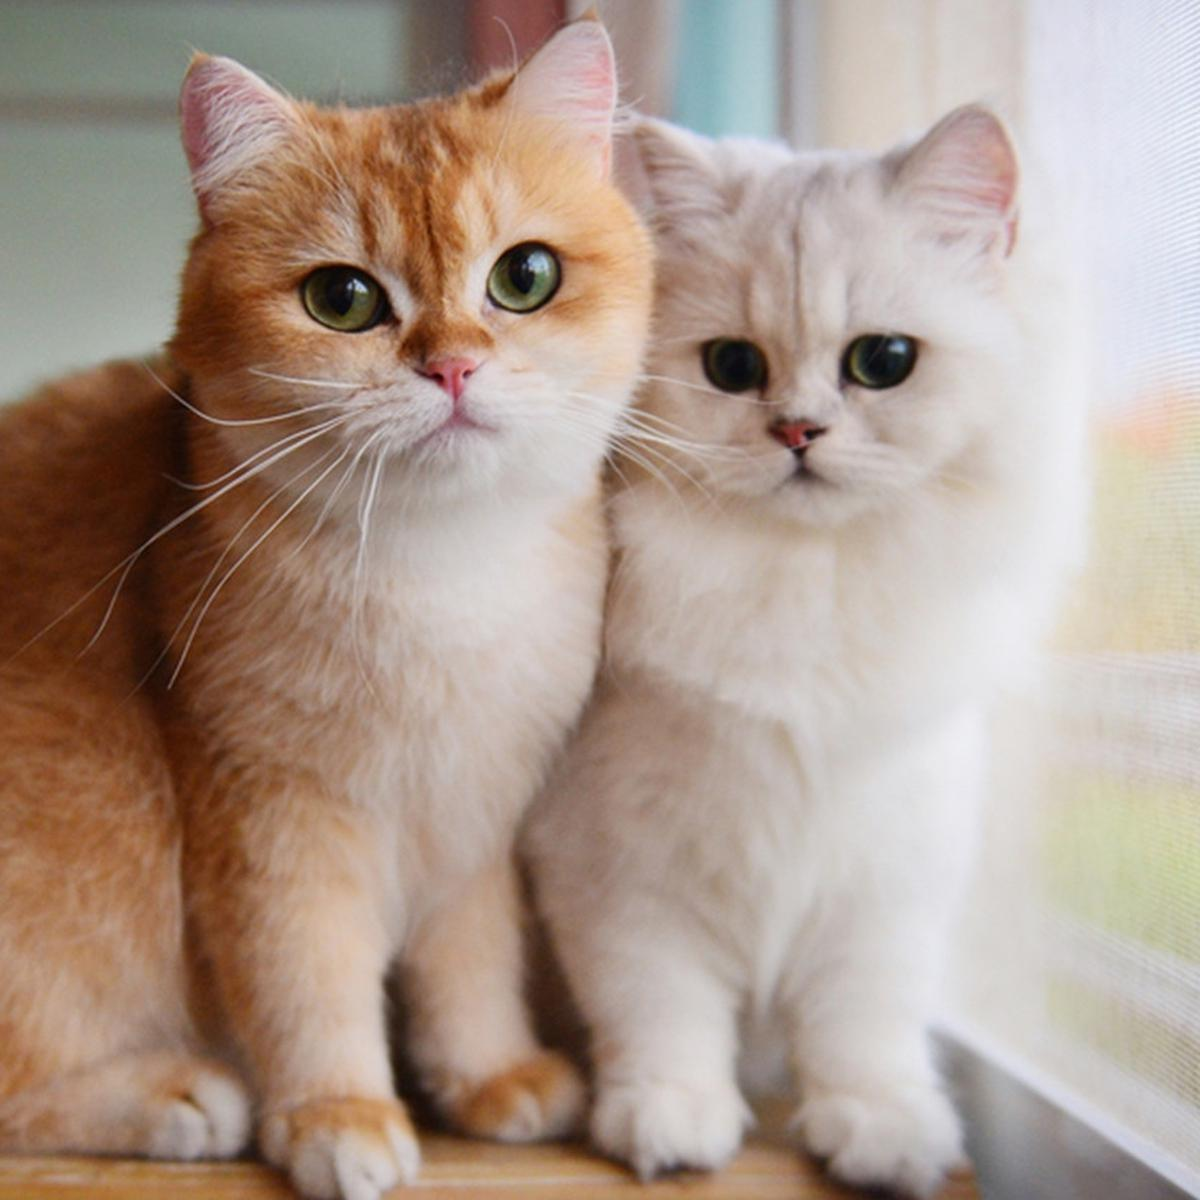
\includegraphics[scale=0.2]{gambar-kucing}
%        \caption{Gambar Kucing Lucu dan Imut}
%    \end{figure}
%\end{lstlisting}

Ukuran gambar dapat diganti dengan mengganti nilai pada scale. Jangan lupa memberikan caption pada setiap gambar. Berikut adalah contoh dari gambar yang telah dimasukkan pada dokumen. Penomoran gambar sudah otomatis dan akan masuk ke daftar gambar juga secara otomatis. Apabila ada beberapa gambar yang akan di embed dengan 1 caption, maka silahkan edit terlebih dahulu dan dijadikan menjadi 1 gambar. Posisi gambar akan pasti setelah dari text ini, apabila ingin mengganti posisinya parameter \textit{H} dapat diganti dengan \textit{h, t, b, p} sesuai kebutuhan.

\begin{figure}[H]
    \centering
    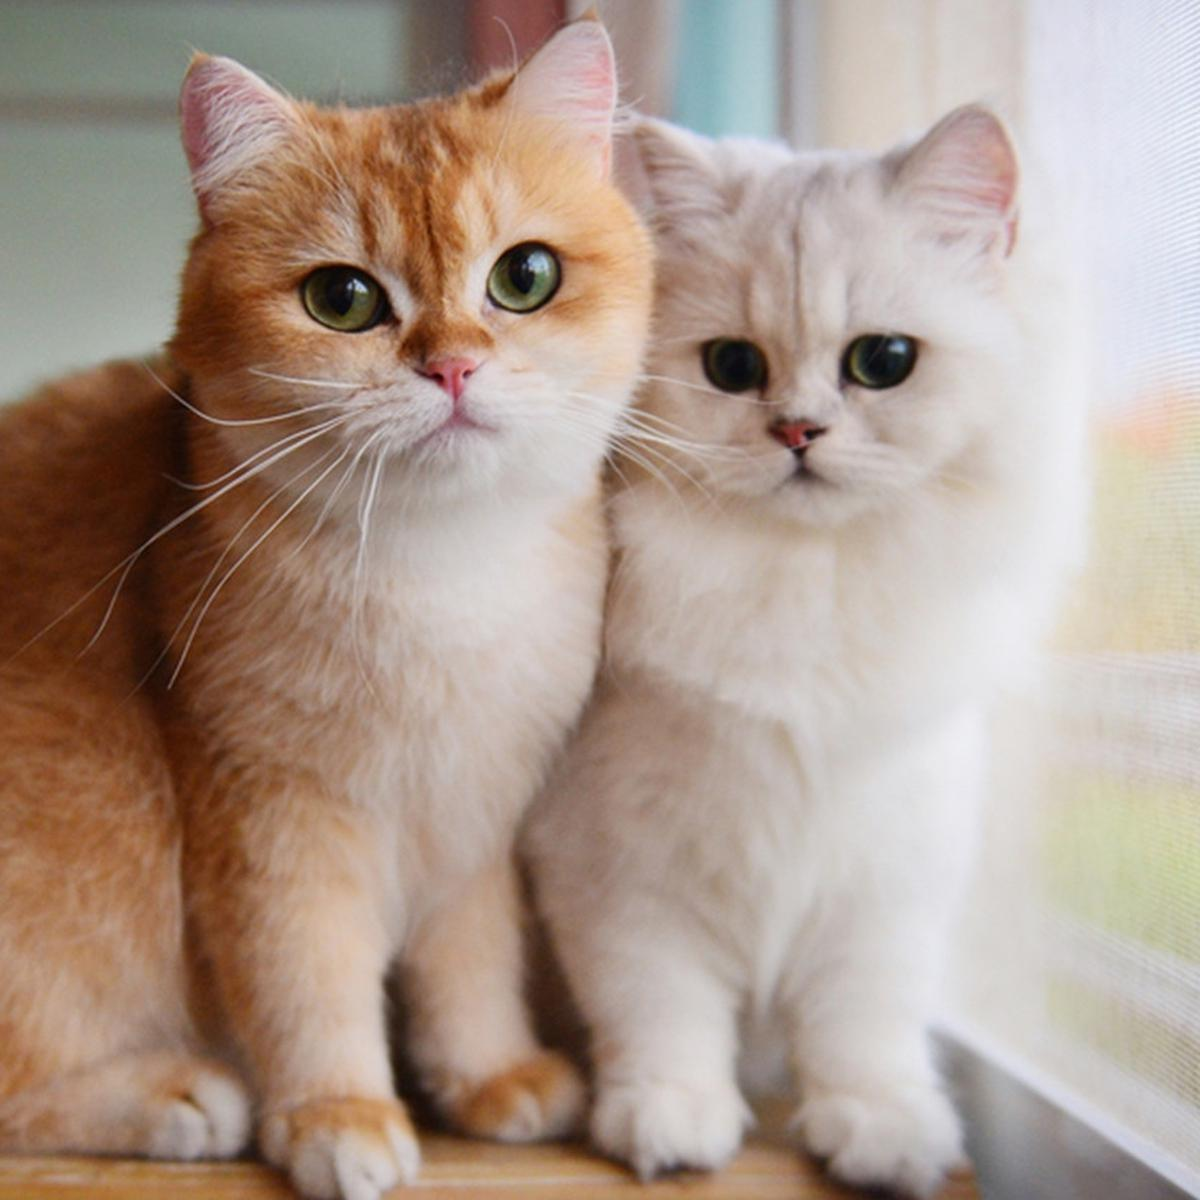
\includegraphics[scale=0.1]{gambar-kucing}
    \caption{Gambar Kucing Lucu dan Imut dengan scala 0.1}
    \label{fig:kucing}
\end{figure}

Setiap gambar harus dimention atau disebutkan didalam bacaan seperti berikut ini \cref{fig:kucing}.

\begin{figure}[H]
    \centering
    
\includegraphics[scale=0.4]{logo-uny}
    \caption{Logo UNY dengan scala 0.4}
    \label{fig:logoUNY}
\end{figure}

Untuk menambahkan gambar secara landscape dapat dilihat pada contoh berikut ini dan jangan lupa selalu menyebutkan nomor gambar disertai penjelasannya seperti ini \cref{fig:logoUNY}.

\begin{sidewaysfigure}[htbp]
	\centering
	
\includegraphics[width=0.6\textwidth]{logo-uny}
	\caption{Logo UNY pada Landscape mode}
    \label{fig:logoUNYlandscape}
\end{sidewaysfigure}

\begin{figure}[H]
    \centering
    \subfigure[]{
     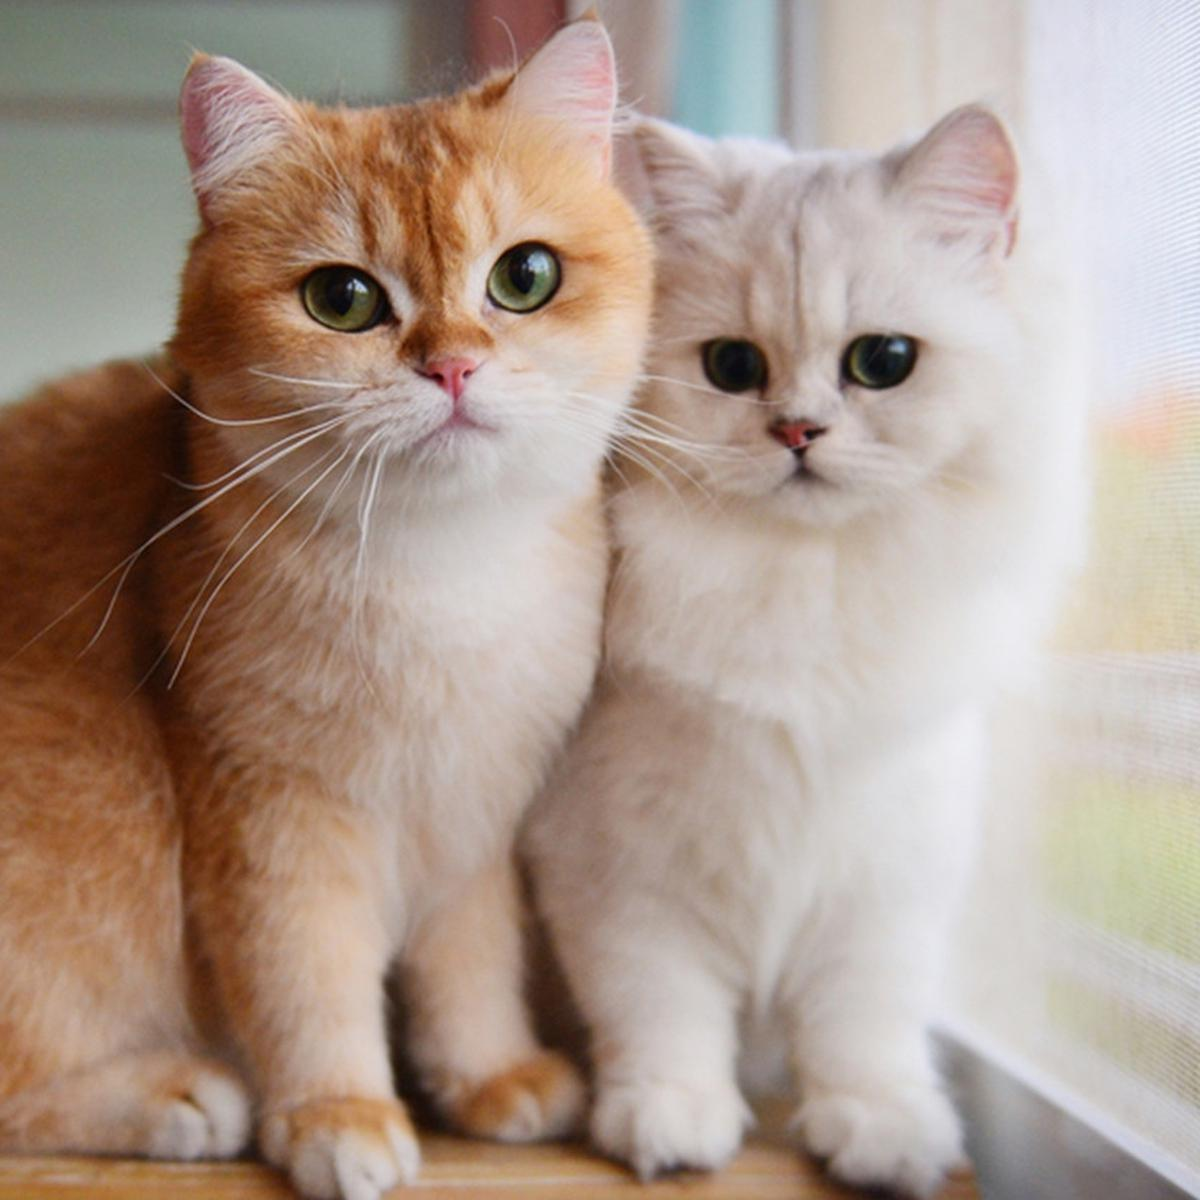
\includegraphics[width=0.4\linewidth]{gambar-kucing}
     }\hspace{0.1\linewidth}
    \subfigure[]{
     
\includegraphics[width=0.4\linewidth]{logo-uny}
    }
    \caption{Dengan menempatkan gambar (a) dan (b), pembaca akan lebih mudah membandingkan keduanya.}
    \label{fig:kucingdanUNY}
\end{figure}

\subsection{Membuat Tabel}
Pada bagian ini akan dijelaskan bagaimana membuat tabel dalam sebuah dokumen \LaTeX. untuk membuat tabel memang agak sedikit sulit, sehingga saya menyarankan menggunakan tool berikut \url{https://www.tablesgenerator.com/} kemudian isikan tabel pada tool generator tersebut dan salin kodenya ke dalam dokumen \LaTeX. Berikut adalah contoh dari sebuah tabel yang telah dibuat. Jangan lupa setiap tabel harus dimention dan dijelaskan dibacaan seperti berikut ini \cref{tab:spekPC}.


\begin{longtable}{|p{2cm}|p{7cm}|}
    \caption{Spesifikasi komputer untuk menjalankan simulator.}
    \label{tab:spekPC} \\
    \hline
    OS     & Ubuntu 20.04.2 LTS             \\ \hline
    Kernel & 5.4.0-80-generic               \\ \hline
    CPU    & Intel i3-8100 (4) @ 3.600GH    \\ \hline
    GPU    & NVIDIA GeForce GTX 1050 Ti     \\ \hline
    RAM    & 7901 MiB                       \\ \hline
\end{longtable}

Kita juga bisa menambahkan tabel yang besar dengan format halaman landscape seperti contoh berikut dan mention tabel seperti berikut ini \cref{tab:landscape} dan berikut ini \cref{tab:tabelx}.
\begin{sidewaysfigure}[htbp]
	\begin{table}[H]
		\caption{Tabel Sederhana}
		\label{tab:landscape}
		\begin{center}
			\begin{tabularx}{0.8\textwidth} {
					|>{\raggedright\arraybackslash}X
					|>{\raggedright\arraybackslash}X
					|>{\raggedright\arraybackslash}X
					|}
				\hline
				$G$     & $\text{dim }G$      & $\text{dim }F$ \\
				\hline
				$SU(N)$ & $N^2 -1$            & $N$            \\
				$SO(N)$ & $\frac{1}{2}N(N-1)$ & $N$            \\
				$Sp(N)$ & $N(2N+1)$           & $2N$           \\
				$E_6$   & $78$                & $27$           \\
				$E_7$   & $133$               & $56$           \\
				$E_8$   & $248$               & $248$          \\
				$F_4$   & $52$                & $6$            \\
				$G_2$   & $14$                & $7$            \\
				\hline
			\end{tabularx}
		\end{center}
	\end{table}
\end{sidewaysfigure}

\begin{table}[H]
	\caption{Tabel Sederhana}
	\label{tab:tabelx}
	\begin{center}
		\begin{tabularx}{0.8\textwidth} {
				|>{\raggedright\arraybackslash}X
				|>{\raggedright\arraybackslash}X
				|>{\raggedright\arraybackslash}X
				|}
			\hline
			$G$     & $\text{dim }G$      & $\text{dim }F$ \\
			\hline
			$SU(N)$ & $N^2 -1$            & $N$            \\
			$SO(N)$ & $\frac{1}{2}N(N-1)$ & $N$            \\
			$Sp(N)$ & $N(2N+1)$           & $2N$           \\
			$E_6$   & $78$                & $27$           \\
			$E_7$   & $133$               & $56$           \\
			$E_8$   & $248$               & $248$          \\
			$F_4$   & $52$                & $6$            \\
			$G_2$   & $14$                & $7$            \\
			\hline
		\end{tabularx}
	\end{center}
\end{table}

\subsection{Menambahkan listing Kode Program}
Berikut adalah beberapa contoh listing kode yang diembed ke dalam dokumen \LaTeX. kita bisa menentukan bahasa pemrograman yang digunakan, misal seperti python. Berikut adalah contoh dari kode java, python, octave, dan C. Selain itu juga banyak paket yang bisa digunakan untuk styling / highlighting sumber kode yang digunakan, apabila dirasa dibutuhkan bisa ditambahkan manual.

\lstinputlisting[caption=Contoh Kode Program Python, label={lst:listing-python}, language=Python]{kode/code_sample.py}

\lstinputlisting[caption=Contoh Kode Program C++, label={lst:listing-cpp}, language=C++]{kode/code_sample.cpp}

\lstinputlisting[caption=Contoh Kode Program Arduino, label={lst:listing-cpp}, language=C++]{kode/code_sample.ino}

\lstinputlisting[caption=Contoh Kode Program Java, label={lst:listing-java}, language=C++]{kode/code_sample.java}


\subsection{Menambahkan Persamaan}
Persamaan tidak lepas dari bidang ilmu teknik dan kadang perlu dituliskan dalam sebuah laporan. Sangat mudah menuliskan persamaan pada sebuah dokumen \LaTeX. Terdapat 2 jenis penulisan persamaan, yaitu inline dengan text seperti contoh ini \(x^2 + y^2 = z^2\) atau seperti ini $E=mc^2$. Jenis lain adalah dituliskan seperti dibawah ini, yang otomatis akan mendapatkan penomoran. Apabila belum familiar dengan kode untuk penulisan persamaan pada \LaTeX bisa menggunakan tool berikut \url{https://latex.codecogs.com/eqneditor/editor.php}. Setiap persamaan harus dimention seperti berikut ini \cref{eq:satu} dan harus dijelaskan terkait persamaan tersebut untuk apa.

\begin{equation}
    \label{eq:satu}
    E=mc^2
\end{equation}

\subsection{Referensi dan Sitasi}
Referensi dan sitasi pada dokumen \LaTeX juga cukup mudah. Silahkan buka file \textit{pustaka.bib} dan amati beberapa contoh penulisan referensi yang ada. Untuk menggenerate bentuk referensi seperti ini dapat menggunakan Mendeley atau Zotero. Mensitasi referensi seperti ini \cite{Kim2006} dapat dilakukan dengan perintah \verb|\cite{nama_label}|.

\section{Section 3.3}
Desain dan Implementasi

\subsection{Subsection 3.3.1}
Bagian ini digunakan apabila dibutuhkan, silahkan bisa ditambah atau dikurangi sesuai kebutuhan.

\subsection{Subsection 3.3.2}
Bagian ini digunakan apabila dibutuhkan, silahkan bisa ditambah atau dikurangi sesuai kebutuhan.

\subsection{Subsection 3.3.3}
Bagian ini digunakan apabila dibutuhkan, silahkan bisa ditambah atau dikurangi sesuai kebutuhan.

\section{Section 3.4}
Desain dan Implementasi

\subsection{Subsection 3.4.1}
Bagian ini digunakan apabila dibutuhkan, silahkan bisa ditambah atau dikurangi sesuai kebutuhan.

\subsection{Subsection 3.4.2}
Bagian ini digunakan apabila dibutuhkan, silahkan bisa ditambah atau dikurangi sesuai kebutuhan.

\subsection{Subsection 3.4.3}
Bagian ini digunakan apabila dibutuhkan, silahkan bisa ditambah atau dikurangi sesuai kebutuhan.

\section{Section 3.5}
Section maupun subsection dapat ditambah atau dikurangi sesuai dengan kebutuhan.

\subsection{Subsection 3.5.1}
Bagian ini digunakan apabila dibutuhkan, silahkan bisa ditambah atau dikurangi sesuai kebutuhan.

\subsection{Subsection 3.5.2}
Bagian ini digunakan apabila dibutuhkan, silahkan bisa ditambah atau dikurangi sesuai kebutuhan.

\subsection{Subsection 3.5.3}
Bagian ini digunakan apabila dibutuhkan, silahkan bisa ditambah atau dikurangi sesuai kebutuhan.
		%==================================================================
% Ini adalah bab 4
% Silahkan edit sesuai kebutuhan, baik menambah atau mengurangi \section, \subsection
%==================================================================

\chapter[PROSES, HASIL, PEMBAHASAN]{\\ PROSES, HASIL, PEMBAHASAN}

\section{Section 4.1}
Hasil adalah bagian dari laporan proyek akhir sarjana terapan yang menjabarkan tentang temuan yang didapat dari pelaksanaan penelitian. Hasil penelitian dapat ditunjukkan dalam bentuk tabel, grafik, atau deskripsi yang menunjukkan data yang didapat dari pengumpulan data. Hasil juga harus dianalisis dan dibahas dalam konteks masalah yang diteliti dan tujuan penelitian.

Dalam laporan proyek akhir sarjana terapan yang meneliti pengaruh perubahan iklim terhadap hasil panen padi, hasil yang didapat dapat ditunjukkan dalam bentuk grafik yang menunjukkan perbandingan hasil panen padi di lokasi yang berbeda dengan kondisi iklim yang berbeda. Hasil ini juga dapat dianalisis dengan menggunakan statistik inferensial untuk mengetahui pengaruh perubahan iklim terhadap hasil panen padi.

Pengujian adalah bagian dari laporan proyek akhir sarjana terapan yang menjabarkan tentang evaluasi dari hasil yang didapat dari pelaksanaan penelitian. Pengujian dilakukan dengan menggunakan metode statistik yang sesuai dengan desain penelitian yang digunakan.

Dalam laporan proyek akhir sarjana terapan yang meneliti pengaruh perubahan iklim terhadap hasil panen padi, pengujian dapat dilakukan dengan menggunakan uji statistik inferensial untuk mengetahui pengaruh perubahan iklim terhadap hasil panen padi. Uji ini dapat dilakukan dengan menggunakan uji-t atau uji-F untuk mengetahui perbedaan yang signifikan antara hasil panen padi di lokasi yang berbeda dengan kondisi iklim yang berbeda.

Hasil dan pengujian dari laporan proyek akhir sarjana terapan harus diinterpretasikan dengan benar dan dibahas dalam konteks masalah yang diteliti dan tujuan penelitian. Selain itu, hasil dan pengujian juga harus dibandingkan dengan hasil penelitian sebelumnya untuk mengetahui keterkaitan dengan penelitian yang telah dilakukan sebelumnya dan memberikan kontribusi baru dalam bidang penelitian terkait.

\subsection{Subsection 4.1.1}
Bagian ini digunakan apabila dibutuhkan, silahkan bisa ditambah atau dikurangi sesuai kebutuhan.

\subsection{Subsection 4.1.2}
Bagian ini digunakan apabila dibutuhkan, silahkan bisa ditambah atau dikurangi sesuai kebutuhan.

\subsection{Subsection 4.1.3}
Bagian ini digunakan apabila dibutuhkan, silahkan bisa ditambah atau dikurangi sesuai kebutuhan.

\section{Section 4.2}
\noindent Hasil dan Pengujian

\subsection{Subsection 4.2.1}
Bagian ini digunakan apabila dibutuhkan, silahkan bisa ditambah atau dikurangi sesuai kebutuhan.

\subsection{Subsection 4.2.2}
Bagian ini digunakan apabila dibutuhkan, silahkan bisa ditambah atau dikurangi sesuai kebutuhan.

\subsection{Subsection 4.2.3}
Bagian ini digunakan apabila dibutuhkan, silahkan bisa ditambah atau dikurangi sesuai kebutuhan.

\section{Section 4.3}
Hasil dan Pengujian

\subsection{Subsection 4.4.1}
Bagian ini digunakan apabila dibutuhkan, silahkan bisa ditambah atau dikurangi sesuai kebutuhan.

\subsection{Subsection 4.4.2}
Bagian ini digunakan apabila dibutuhkan, silahkan bisa ditambah atau dikurangi sesuai kebutuhan.

\subsection{Subsection 4.3.3}
Bagian ini digunakan apabila dibutuhkan, silahkan bisa ditambah atau dikurangi sesuai kebutuhan.

\section{Section 4.4}
Hasil dan Pengujian

\subsection{Subsection 4.4.1}
Bagian ini digunakan apabila dibutuhkan, silahkan bisa ditambah atau dikurangi sesuai kebutuhan.

\subsection{Subsection 4.4.2}
Bagian ini digunakan apabila dibutuhkan, silahkan bisa ditambah atau dikurangi sesuai kebutuhan.

\subsection{Subsection 4.4.3}
Bagian ini digunakan apabila dibutuhkan, silahkan bisa ditambah atau dikurangi sesuai kebutuhan.

\section{Section 4.5}
Hasil dan Pengujian

\subsection{Subsection 4.5.1}
Bagian ini digunakan apabila dibutuhkan, silahkan bisa ditambah atau dikurangi sesuai kebutuhan.

\subsection{Subsection 4.5.2}
Bagian ini digunakan apabila dibutuhkan, silahkan bisa ditambah atau dikurangi sesuai kebutuhan.

\subsection{Subsection 4.5.3}
Bagian ini digunakan apabila dibutuhkan, silahkan bisa ditambah atau dikurangi sesuai kebutuhan.
		%==================================================================
% Ini adalah bab 5
% Silahkan edit sesuai kebutuhan, baik menambah atau mengurangi \section, \subsection
%==================================================================

\chapter[SIMPULAN DAN SARAN]{\\ SIMPULAN DAN SARAN}

\section{Simpulan}
Kesimpulan adalah bagian penting dari laporan proyek akhir yang menjabarkan tentang temuan yang didapat dari pelaksanaan penelitian dan menjawab masalah yang diteliti sesuai dengan tujuan penelitian. Kesimpulan harus sesuai dengan hasil yang didapat dan dibahas dalam konteks masalah yang diteliti.

Dalam laporan proyek akhir yang meneliti pengaruh perubahan iklim terhadap hasil panen padi, kesimpulan dapat ditarik berdasarkan hasil penelitian yang didapat. Contohnya, jika hasil penelitian menunjukkan bahwa perubahan iklim berpengaruh negatif terhadap hasil panen padi, maka kesimpulan yang dapat ditarik adalah perubahan iklim merupakan faktor yang menurunkan hasil panen padi. Selain itu, kesimpulan juga dapat memberikan saran untuk meningkatkan hasil panen padi yang terdampak oleh perubahan iklim, seperti dengan mengimplementasikan teknologi pertanian yang sesuai atau dengan mengubah pola tanam.

Kesimpulan juga harus dibahas dalam konteks masalah yang diteliti dan tujuan penelitian. Selain itu, kesimpulan juga harus dibandingkan dengan hasil penelitian sebelumnya untuk mengetahui keterkaitan dengan penelitian yang telah dilakukan sebelumnya dan memberikan kontribusi baru dalam bidang penelitian terkait.

Secara keseluruhan, kesimpulan adalah bagian penting dari laporan proyek akhir yang membantu dalam menjabarkan temuan yang didapat dari pelaksanaan penelitian dan menjawab masalah yang diteliti sesuai dengan tujuan penelitian. Kesimpulan harus sesuai dengan hasil yang didapat dan dibahas dalam konteks masalah yang diteliti dan tujuan penelitian. Selain itu, kesimpulan juga harus memberikan saran untuk pengembangan lebih lanjut di bidang yang diteliti dan memberikan kontribusi baru dalam bidang penelitian terkait.

Kesimpulan juga harus dibuat dengan jelas dan ringkas, namun tetap mencakup semua aspek yang diteliti dalam laporan proyek akhir. Selain itu, kesimpulan juga harus dibuat dengan objektif dan tidak mengambil kesimpulan yang tidak didukung oleh data atau hasil penelitian yang didapat.

Secara keseluruhan kesimpulan dari laporan proyek akhir harus memenuhi kriteria yang diharapkan dari laporan proyek akhir yaitu memberikan gambaran yang jelas tentang proses penelitian yang dilakukan, hasil yang didapat, dan kesimpulan yang ditarik serta saran yang diberikan.

\section{Saran}
Saran adalah bagian penting dari laporan proyek akhir yang menjabarkan tentang rekomendasi yang dapat dilakukan untuk pengembangan lebih lanjut dari temuan yang didapat dari pelaksanaan penelitian. Saran harus dibahas dalam konteks masalah yang diteliti dan tujuan penelitian.

Dalam laporan proyek akhir yang meneliti pengaruh perubahan iklim terhadap hasil panen padi, saran dapat diberikan untuk pengembangan lebih lanjut dalam bidang pertanian, seperti:
\begin{packed_item}
    \item Implementasi teknologi pertanian yang sesuai untuk meningkatkan hasil panen padi yang terdampak oleh perubahan iklim
    \item Penelitian lebih lanjut tentang pengaruh perubahan iklim terhadap hasil panen padi di lokasi yang berbeda dengan kondisi iklim yang berbeda
    \item Pembentukan kebijakan pertanian yang sesuai untuk mengatasi masalah perubahan iklim terhadap hasil panen padi
    \item Pendidikan dan sosialisasi tentang perubahan iklim dan cara-cara untuk mengatasinya bagi petani dan masyarakat.
\end{packed_item}

Saran juga harus dibahas dalam konteks masalah yang diteliti dan tujuan penelitian, serta dibandingkan dengan hasil penelitian sebelumnya untuk mengetahui keterkaitan dengan penelitian yang telah dilakukan sebelumnya dan memberikan kontribusi baru dalam bidang penelitian terkait.

Secara keseluruhan, saran adalah bagian penting dari laporan proyek akhir yang membantu dalam memberikan rekomendasi untuk pengembangan lebih lanjut dari temuan yang didapat dari pelaksanaan penelitian. Saran harus dibahas dalam konteks masalah yang diteliti dan tujuan penelitian serta ditujukan untuk memecahkan masalah yang diteliti dan memberikan solusi yang efektif. Saran juga harus dibuat dengan objektif dan tidak berpihak, serta dapat diimplementasikan dalam konteks yang sesuai.
		\chapter[Penulisan dengan \LaTeX - INI HANYA TUTORIAL]{\\ Penulisan dengan \LaTeX  - INI HANYA TUTORIAL}

\section{Membuat List atau Daftar}
Terdapat 2 cara yaitu dengan list yang terdapat penomoran 1,2,3 dst atau dengan bullet poin. Secara detail dapat dibaca pada subsection di bawah.
\subsection{List atau Daftar dengan \texttt{packed\_enum}}
Lingkungan \texttt{packed\_enum} digunakan untuk membuat daftar bernomor dengan jarak yang lebih rapat antar item. Ini sangat berguna untuk menampilkan langkah atau tahapan yang memiliki urutan. Berikut adalah contoh penggunaannya:

\begin{lstlisting}
    \begin{packed_enum}
        \item Langkah pertama adalah mengidentifikasi masalah yang ingin diselesaikan.
        \item Langkah kedua melibatkan analisis kebutuhan.
        \item Langkah ketiga adalah mengembangkan ide dan solusi alternatif.
        \item Langkah keempat adalah melakukan pengujian awal untuk mengevaluasi performa.
    \end{packed_enum}
\end{lstlisting}
    
Hasilnya akan tampak seperti berikut:
\begin{packed_enum}
    \item Langkah pertama adalah mengidentifikasi masalah yang ingin diselesaikan.
    \item Langkah kedua melibatkan analisis kebutuhan.
    \item Langkah ketiga adalah mengembangkan ide dan solusi alternatif.
    \item Langkah keempat adalah melakukan pengujian awal untuk mengevaluasi performa.
\end{packed_enum}

\subsection{List atau Daftar dengan \texttt{packed\_item}}
Lingkungan \texttt{packed\_item} digunakan untuk membuat daftar berpoin dengan jarak antar item yang lebih rapat, cocok untuk poin-poin yang tidak memerlukan urutan tertentu. Berikut adalah contoh penggunaannya:

\begin{lstlisting}
    \begin{packed_item}
        \item Meningkatkan kualitas sensor untuk akurasi yang lebih baik.
        \item Menambahkan modul komunikasi untuk kontrol jarak jauh.
        \item Mengoptimalkan kode untuk efisiensi.
        \item Menambah fitur penghematan energi.
    \end{packed_item}
\end{lstlisting}

Hasilnya akan tampak seperti berikut:
\begin{packed_item}
    \item Meningkatkan kualitas sensor untuk akurasi yang lebih baik.
    \item Menambahkan modul komunikasi untuk kontrol jarak jauh.
    \item Mengoptimalkan kode untuk efisiensi.
    \item Menambah fitur penghematan energi.
\end{packed_item}

\section{Menuliskan Kode Program dengan Listing}
Lingkungan \texttt{lstlisting} memungkinkan kita untuk menuliskan atau menyisipkan kode Python, C++, Arduino, Java atau lainnya dalam dokumen LaTeX dengan format yang rapi dan terstruktur. Pada bagian ini, kita akan melihat dua cara untuk menuliskan kode Python: secara langsung di dalam dokumen dan dengan mengambil dari file eksternal.

\Cref{lst:python_direct} menunjukkan fungsi Python yang menghitung faktorial dari sebuah angka. Kode ini ditulis langsung di dalam dokumen LaTeX menggunakan lingkungan \texttt{lstlisting} dengan format diawali dengan \texttt{\textbackslash begin\{lstlisting\}[language=Python, caption=Contoh Kode Python Langsung, label=lst:python\_direct]} dan diakhiri dengan \texttt{\textbackslash end\{lstlisting\}}, dimana:
\begin{packed_item}
    \item \texttt{language=Python}: Mengatur pewarnaan sintaksis untuk Python.
    \item \texttt{caption}: Menambahkan keterangan di atas kode untuk menjelaskan isi kode.
    \item \texttt{label}: Menambahkan label untuk memudahkan referensi kode dalam dokumen.
\end{packed_item}

\begin{lstlisting}[language=Python, caption=Contoh Kode Python Langsung, label=lst:python_direct]
    def factorial(n):
        if n == 0:
            return 1
        else:
            return n * factorial(n-1)
\end{lstlisting}

Jika Anda memiliki file kode Python di folder tertentu (misalnya, di \texttt{kode/code\_sample.py}), Anda bisa menyisipkan kode tersebut langsung ke dalam dokumen LaTeX menggunakan perintah \texttt{\textbackslash lstinputlisting}. Berikut \cref{lst:python_file} dengan format penulisan \texttt{\textbackslash lstinputlisting[language=Python, caption=Contoh Kode Python dari File, label=lst:python\_file]\{kode/code\_sample.py\}}, dimana:
\begin{packed_item}
    \item \texttt{language=Python}: Mengatur pewarnaan sintaksis untuk Python.
    \item \texttt{caption}: Menambahkan keterangan untuk kode yang diambil dari file.
    \item \texttt{label}: Menambahkan label untuk referensi.
    \item \texttt{\{kode/code\_sample.py\}}: Menentukan path atau lokasi file Python yang akan disisipkan. Pastikan file berada di dalam folder \texttt{kode} atau path yang sesuai.
\end{packed_item}

\lstinputlisting[language=Python, caption=Contoh Kode Python dari File, label=lst:python_file]{kode/code_sample.py}

\section{Menambahkan Gambar}
Untuk menambahkan gambar hal yang harus dilakukan adalah:
\begin{packed_enum}
    \item Menyalin file gambar (dalam format jpg \/ png) ke dalam folder \textit{gambar}
    \item Mengganti nama file dari gambar agar mudah dikenali, jangan diberi nama gambar-1,-2, dst
    \item Memasukkan seperti \cref{lst:kode_gambar}
\end{packed_enum}

\begin{lstlisting}[language=TeX, caption=Kode untuk Menyisipkan Gambar dalam Dokumen, label=lst:kode_gambar]
    \begin{figure}[H]
        \centering
        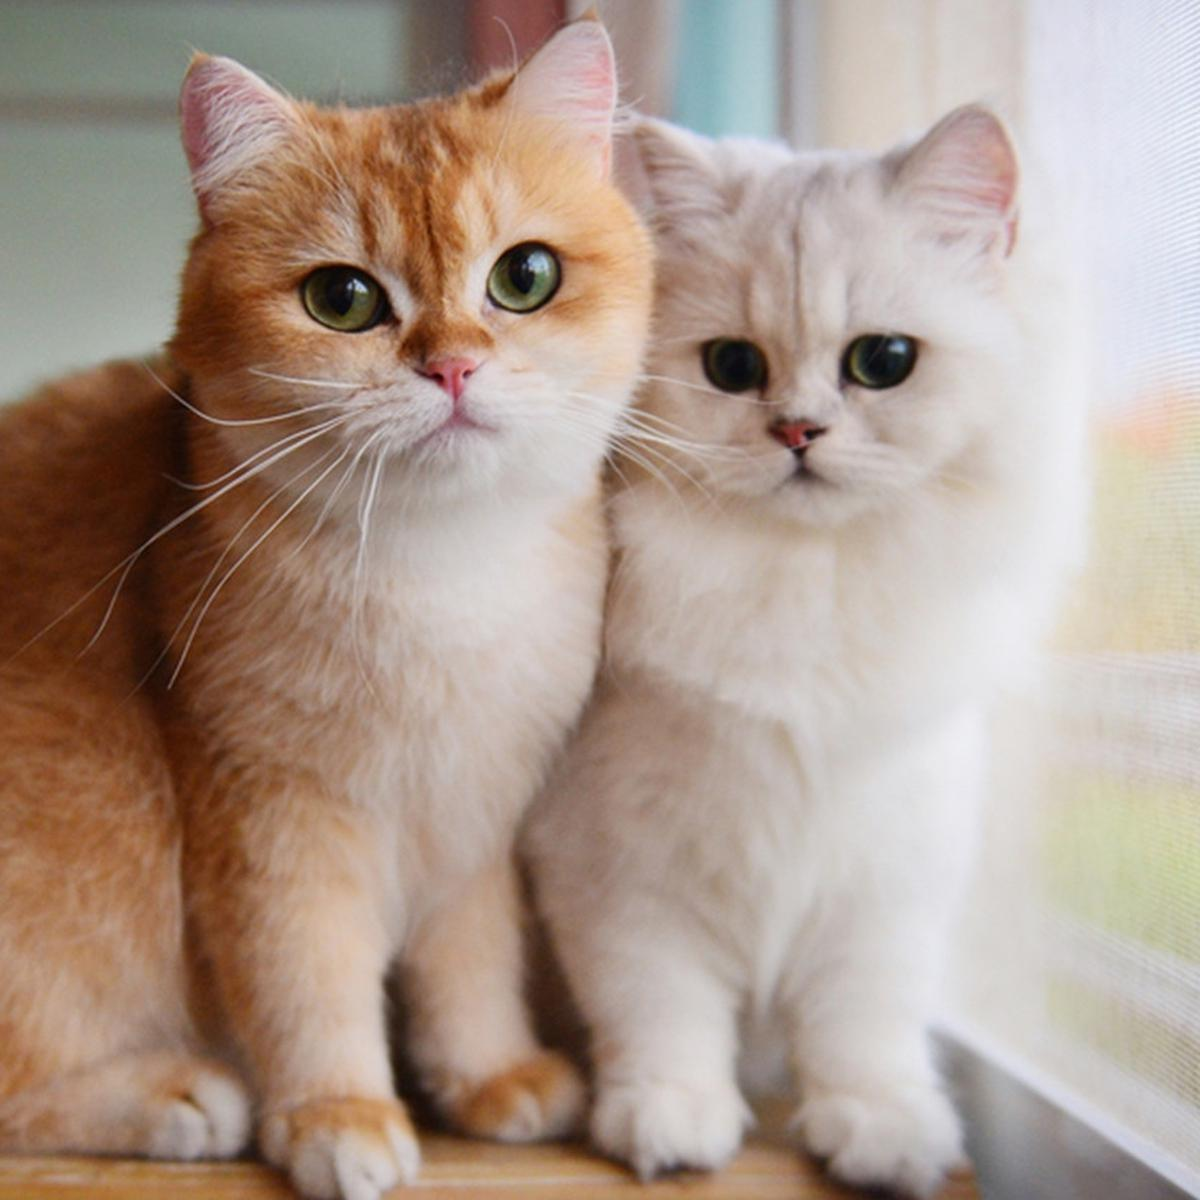
\includegraphics[scale=0.2]{gambar-kucing.jpg}
        \caption{Gambar Kucing Lucu dan Imut}
        \label{fig:kucing}
    \end{figure}
\end{lstlisting}

\noindent Berikut adalah penjelasan dari setiap baris pada kode di atas:

\begin{packed_enum}
    \item \texttt{\textbackslash begin\{figure\}[H] ... \textbackslash end\{figure\}}: Membuat lingkungan \texttt{figure} untuk menyisipkan gambar. Parameter \texttt{[H]} digunakan agar gambar diletakkan tepat di posisi yang ditentukan dalam kode. Opsi \textit{H} dapat diganti dengan \textit{h, t, b, p} sesuai kebutuhan.
    \item \texttt{\textbackslash centering}: Mengatur gambar agar berada di tengah halaman.
    \item \texttt{\textbackslash includegraphics[scale=0.2]\{gambar-kucing.jpg\}}: Memasukkan gambar dengan nama file \texttt{gambar-kucing.jpg}. Parameter \texttt{scale=0.2} mengatur ukuran gambar pada 20\% dari ukuran aslinya. Ubah nilainya untuk memperbesar atau memperkecil gambar.
    \item \texttt{\textbackslash caption\{Gambar Kucing Lucu dan Imut\}}: Menambahkan keterangan (caption) di bawah gambar yang akan muncul di Daftar Gambar dan disertai nomor gambar secara otomatis.
    \item \texttt{\textbackslash label\{fig:kucing\}}: Memberikan label pada gambar untuk merujuk gambar ini dalam teks menggunakan \texttt{\textbackslash cref\{fig:kucing\}} atau \texttt{\textbackslash ref\{fig:kucing\}} yang menghasilkan "Gambar 1" atau penomoran gambar sesuai urutan.
\end{packed_enum}

Hasilnya adalah terlihat seperti pada \cref{fig:kucing}.

\begin{figure}[H]
    \centering
    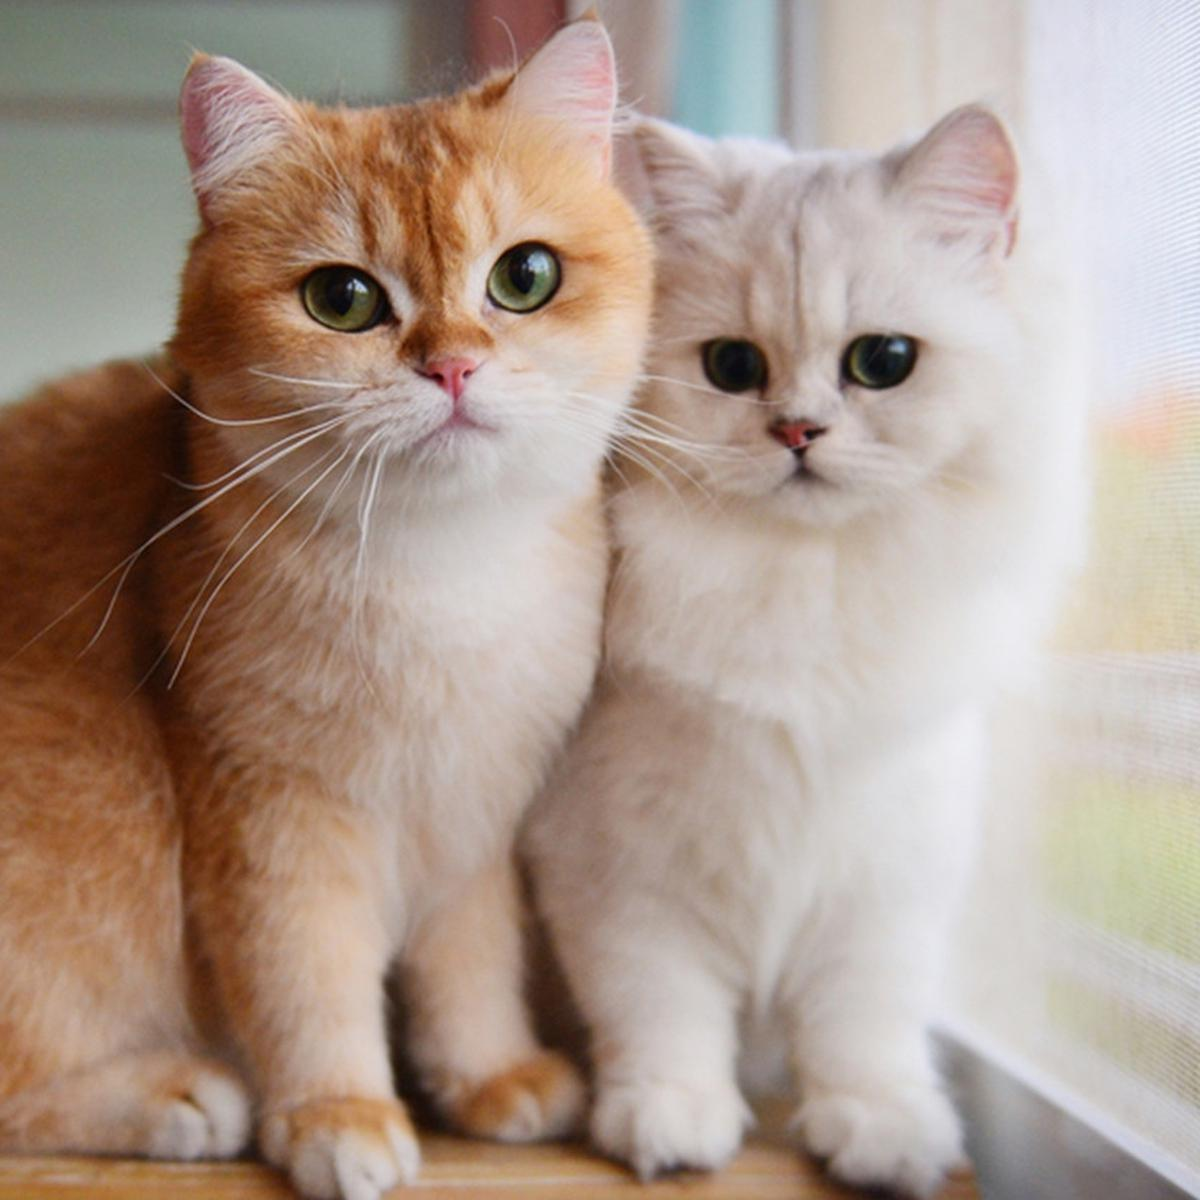
\includegraphics[scale=0.1]{gambar-kucing}
    \caption{Gambar Kucing Lucu dan Imut dengan scala 0.1}
    \label{fig:kucing}
\end{figure}

Setiap gambar harus dimention atau disebutkan didalam bacaan seperti berikut ini \cref{fig:kucing} dan \cref{fig:logoUNY}.

\begin{figure}[H]
    \centering
    
\includegraphics[scale=0.4]{logo-uny}
    \caption{Logo UNY dengan scala 0.4}
    \label{fig:logoUNY}
\end{figure}

Untuk menyisipkan beberapa gambar dalam satu kelompok dan satu caption utama, kita dapat menggunakan lingkungan \texttt{subfigure} di dalam lingkungan \texttt{figure}. Metode ini sangat bermanfaat jika kita ingin menyusun beberapa gambar berukuran kecil dalam satu baris atau kolom, dengan setiap gambar diberi caption masing-masing dan satu caption utama untuk keseluruhan gambar.

Kode berikut menunjukkan cara menyusun tiga gambar secara berdampingan dengan satu caption utama.

\begin{lstlisting}[language=TeX, caption=Kode untuk Menyisipkan Gambar dalam Dokumen dengan Subfigure, label=lst:kode_gambar_multi]
    \begin{figure}
        \centering
        \begin{subfigure}[b]{0.3\textwidth}
            \centering
            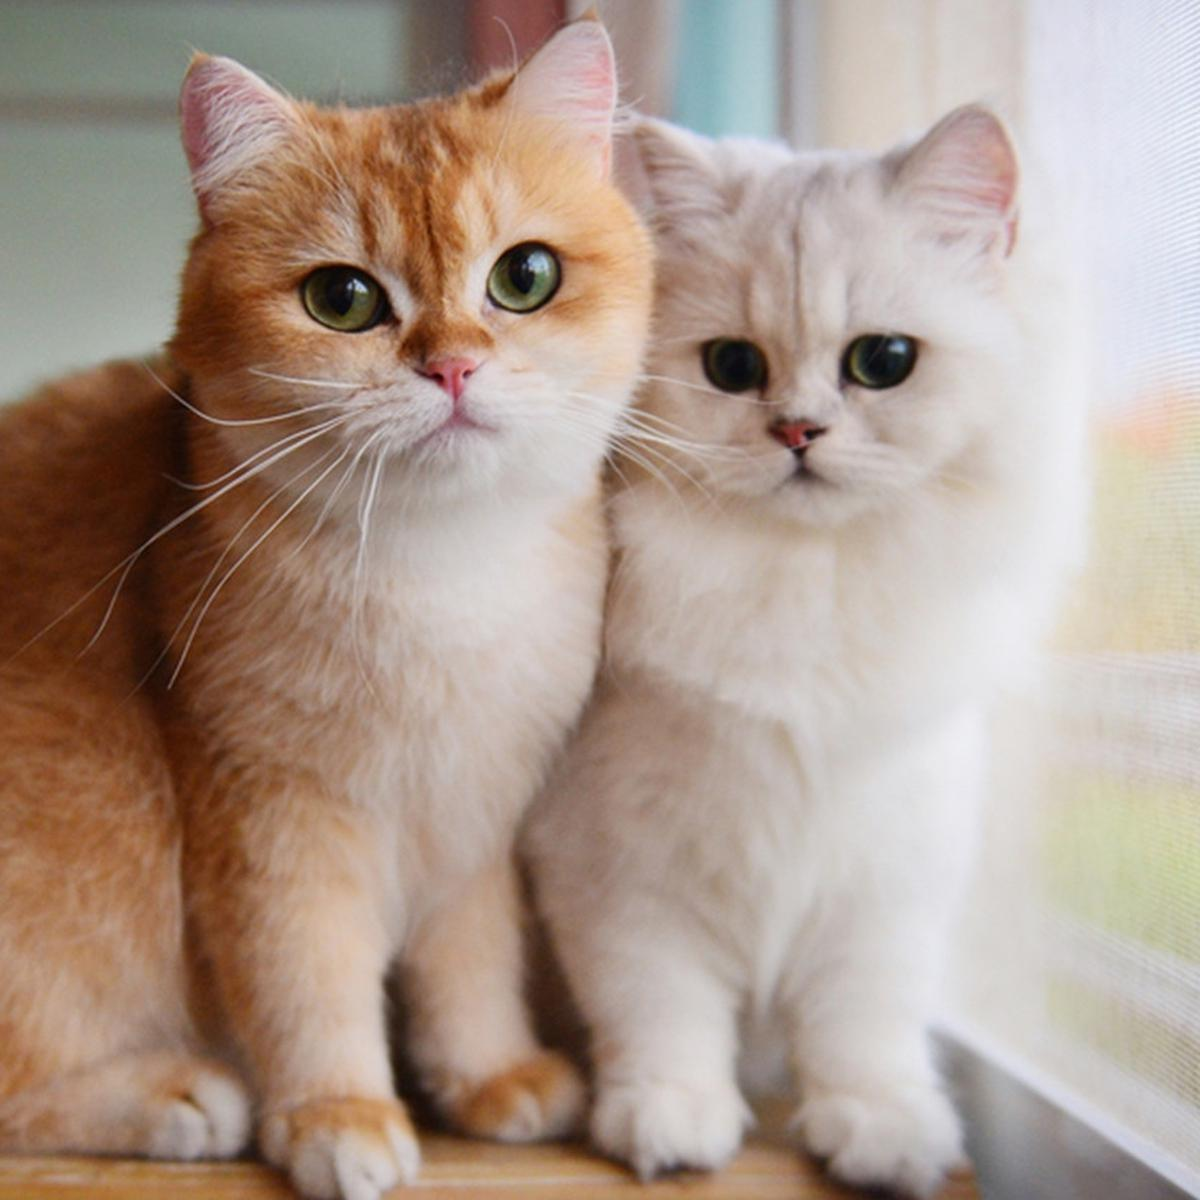
\includegraphics[width=\linewidth]{gambar-kucing.jpg}
            \caption{Kucing Lucu 1}
            \label{fig:kucing-a}
        \end{subfigure}
        \hfill
        \begin{subfigure}[b]{0.3\textwidth}
            \centering
            
\includegraphics[width=\linewidth]{logo-uny.png}
            \caption{Logo UNY}
            \label{fig:logo-uny-b}
        \end{subfigure}
        \hfill
        \begin{subfigure}[b]{0.3\textwidth}
            \centering
            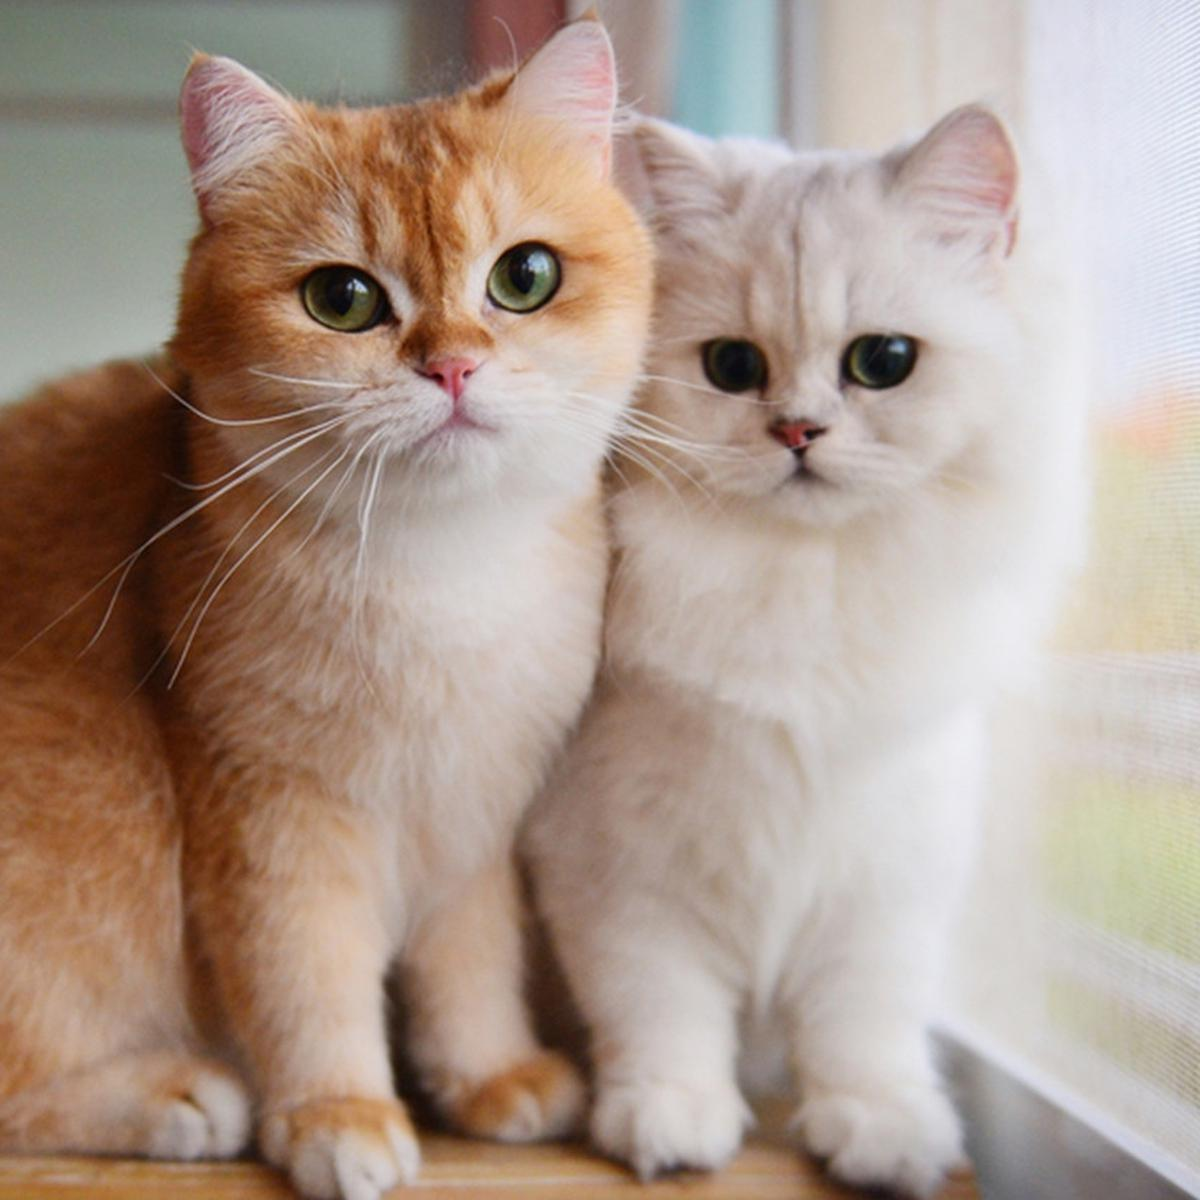
\includegraphics[width=\linewidth]{gambar-kucing.jpg}
            \caption{Kucing Lucu 2}
            \label{fig:kucing-c}
        \end{subfigure}
        \caption{Beberapa gambar yang disusun menjadi 1 bagian dengan penomoran (a), (b), dan (c)}
        \label{fig:kucingdanUNY}
    \end{figure}
\end{lstlisting}

\noindent Berikut adalah penjelasan dari setiap bagian kode di atas:

\begin{packed_enum}
    \item \texttt{\textbackslash begin\{figure\} ... \textbackslash end\{figure\}}: Lingkungan \texttt{figure} utama yang berfungsi sebagai wadah untuk menyisipkan beberapa gambar dalam satu bagian.
    
    \item \texttt{\textbackslash begin\{subfigure\}[b]\{0.3\textbackslash textwidth\} ... \textbackslash end\{subfigure\}}: Lingkungan \texttt{subfigure} digunakan untuk setiap gambar yang ingin disusun dalam satu bagian. Parameter \texttt{0.3\textbackslash textwidth} mengatur lebar setiap gambar menjadi sepertiga dari lebar teks, sehingga tiga gambar dapat ditampilkan berdampingan dalam satu baris.
    
    \item \texttt{\textbackslash includegraphics[width=\textbackslash linewidth]\{gambar-nama\}}: Memasukkan setiap gambar dengan lebar yang sesuai dengan lebar yang telah ditentukan untuk \texttt{subfigure}. 
        \begin{packed_enum}
            \item Gambar pertama menggunakan file \texttt{gambar-kucing}, dengan caption "Kucing Lucu 1".
            \item Gambar kedua menggunakan file \texttt{logo-uny}, dengan caption "Logo UNY".
            \item Gambar ketiga juga menggunakan file \texttt{gambar-kucing}, dengan caption "Kucing Lucu 2".
        \end{packed_enum}
    
    \item \texttt{\textbackslash hfill}: Menyisipkan ruang kosong antar gambar, agar setiap \texttt{subfigure} memiliki jarak yang merata.
    
    \item \texttt{\textbackslash caption\{...\}}: Caption utama yang menjelaskan ketiga gambar sekaligus. Caption ini akan ditampilkan di bawah semua gambar dalam lingkungan \texttt{figure}.

    \item \texttt{\textbackslash label\{fig:kucingdanUNY\}}: Memberikan label untuk keseluruhan kelompok gambar, sehingga kita bisa merujuk ke seluruh bagian gambar ini dalam teks dengan \texttt{\textbackslash cref\{fig:kucingdanUNY\}}.
\end{packed_enum}

Dengan menggunakan metode ini, Anda dapat menyisipkan beberapa gambar dalam satu bagian dengan satu caption utama seperti pada \cref{fig:kucingdanUNY}. Setiap gambar dapat memiliki caption terpisah dan nomor (misalnya, (a), (b), (c)), sehingga rujukan spesifik untuk masing-masing gambar dapat dibuat, seperti \texttt{\textbackslash cref\{fig:kucing-a\}} untuk merujuk ke \cref{fig:kucing-a}.

\begin{figure}
    \centering
    \begin{subfigure}[b]{0.3\textwidth}
        \centering
        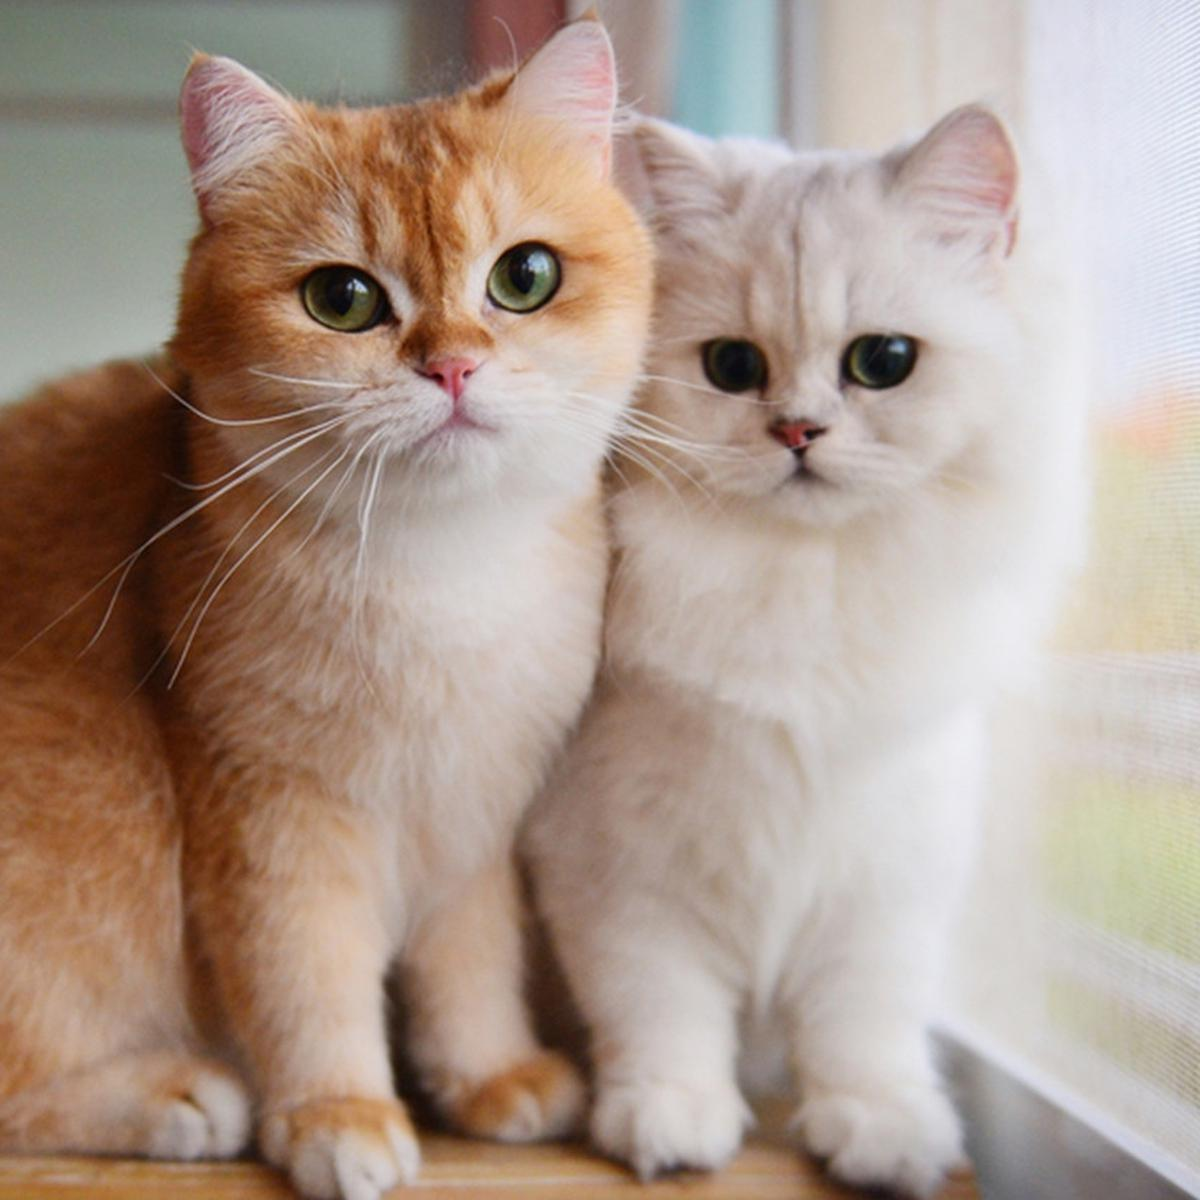
\includegraphics[width=\linewidth]{gambar-kucing.jpg}
        \caption{Kucing Lucu 1}
        \label{fig:kucing-a}
    \end{subfigure}
    \hfill
    \begin{subfigure}[b]{0.3\textwidth}
        \centering
        
\includegraphics[width=\linewidth]{logo-uny.png}
        \caption{Logo UNY}
        \label{fig:logo-uny-b}
    \end{subfigure}
    \hfill
    \begin{subfigure}[b]{0.3\textwidth}
        \centering
        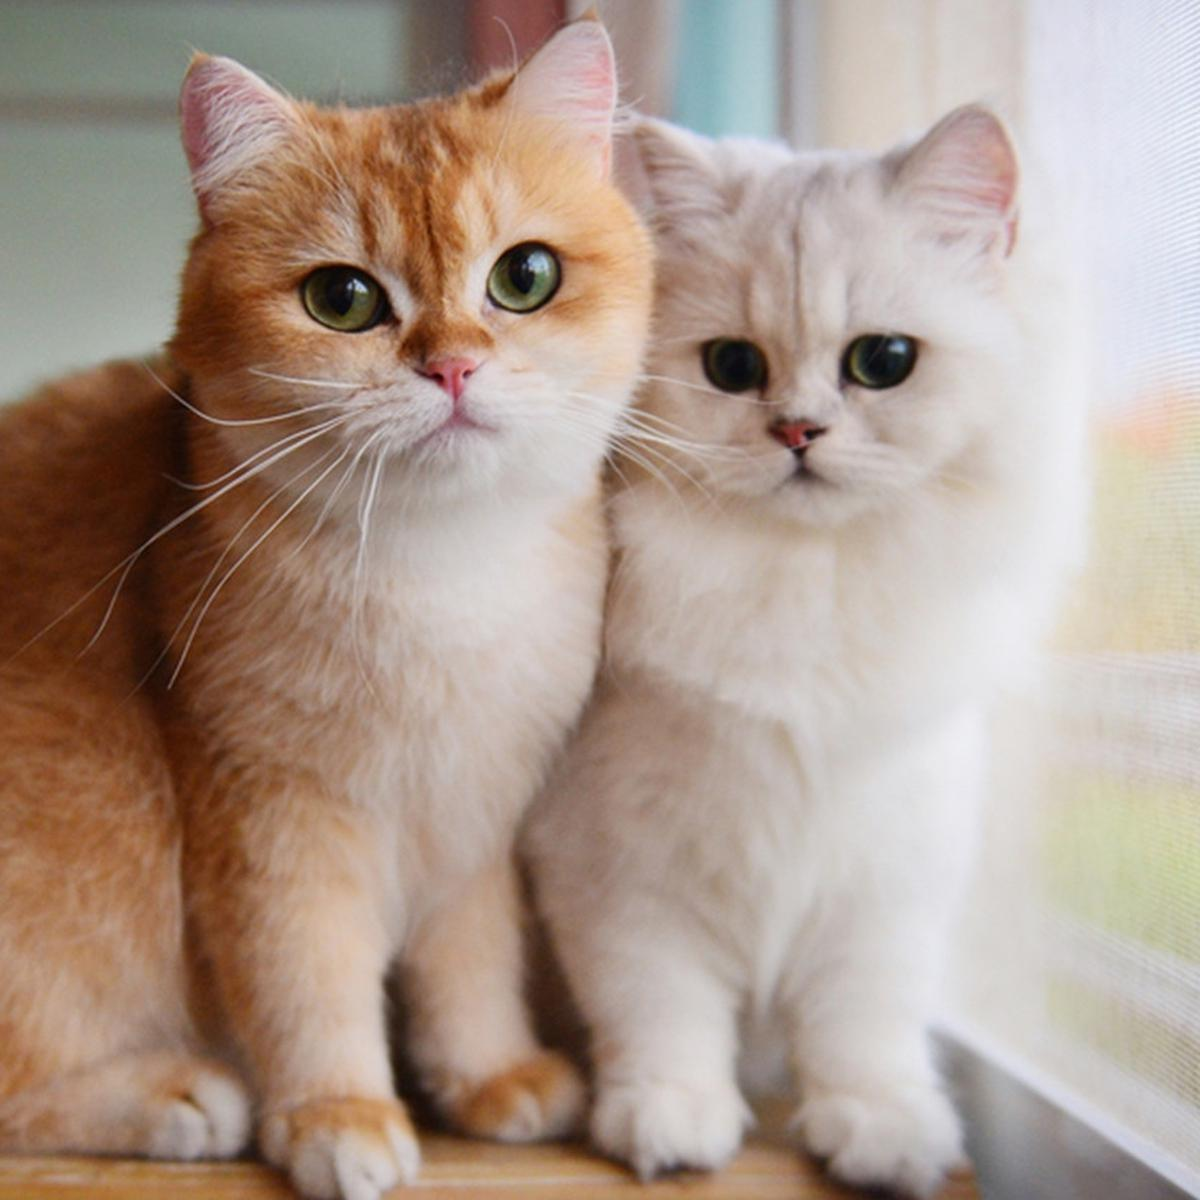
\includegraphics[width=\linewidth]{gambar-kucing.jpg}
        \caption{Kucing Lucu 2}
        \label{fig:kucing-c}
    \end{subfigure}
    \caption{Beberapa gambar yang disusun menjadi 1 bagian dengan penomoran (a), (b), dan (c)}
    \label{fig:kucingdanUNY}
\end{figure}

\section{Membuat Grafik dengan Tikz}
TikZ adalah sebuah paket LaTeX yang digunakan untuk membuat grafik vektor. Berikut adalah beberapa contoh dasar penggunaan TikZ.

\subsection{Menggambar Garis dan Bentuk Dasar}
Untuk menggambar garis dan bentuk dasar, kita bisa menggunakan perintah-perintah berikut:
\begin{lstlisting}[language=TeX, caption=Kode untuk Menggambar Garis dan Bentuk Dasar, label=lst:Menggambar Garis dan Bentuk Dasar]
    \begin{figure}[H]
        \centering
        \begin{tikzpicture}
            \draw (0,0) -- (2,0);
            \draw (0,0) rectangle (2,2);
            \draw (1,1) circle (1);
        \end{tikzpicture}
        \caption{Menggambar Garis dan Bentuk Dasar}
        \label{fig:tikzExample}
    \end{figure}
\end{lstlisting}

\begin{figure}[H]
    \centering
    \begin{tikzpicture}
        \draw (0,0) -- (2,0);
        \draw (0,0) rectangle (2,2);
        \draw (1,1) circle (1);
    \end{tikzpicture}
    \caption{Menggambar Garis dan Bentuk Dasar}
    \label{fig:tikzExample}
\end{figure}

Pada Gambar \ref{fig:tikzExample} dapat dilihat contoh gambar sederhana.

\subsection{Menggambar Grafik Fungsi}
TikZ juga bisa digunakan untuk menggambar grafik fungsi matematika:
\begin{lstlisting}[language=TeX, caption=Kode untuk Menggambar Grafik Fungsi, label=lst:Menggambar Grafik Fungsi]
    \begin{figure}[H]
        \centering
        \begin{tikzpicture}
            \begin{axis}[
                axis lines = middle,
                xlabel = $x$,
                ylabel = {$f(x)$},
                title = {Grafik Fungsi Kuadrat},
                grid = major,
                xmin = -10, 
                xmax = 10,
                ymin = 0, 
                ymax = 100
            ]
            \addplot [
                domain=-10:10, 
                samples=100, 
                color=blue,
            ]
            {x^2};
            \end{axis}
        \end{tikzpicture}
        \caption{Grafik fungsi \( f(x) = x^2 \) dengan domain \( [-10, 10] \)}
        \label{fig:grafik_kuadrat}
    \end{figure}
\end{lstlisting}

\begin{figure}[H]
    \centering
    \begin{tikzpicture}
        \begin{axis}[
            axis lines = middle,
            xlabel = $x$,
            ylabel = {$f(x)$},
            title = {Grafik Fungsi Kuadrat},
            grid = major,
            xmin = -10, 
            xmax = 10,
            ymin = 0, 
            ymax = 100
        ]
        \addplot [
            domain=-10:10, 
            samples=100, 
            color=blue,
        ]
        {x^2};
        \end{axis}
    \end{tikzpicture}
    \caption{Grafik fungsi \( f(x) = x^2 \) dengan domain \( [-10, 10] \)}
    \label{fig:grafik_kuadrat}
\end{figure}

Pada Gambar \ref{fig:grafik_kuadrat} ditunjukkan grafik fungsi kuadrat.

\subsection{Menggambar Diagram Alir}
TikZ juga mendukung pembuatan diagram alir (flowchart):
\begin{lstlisting}[language=TeX, caption=Kode untuk Menggambar Diagram Alir, label=lst:Menggambar Diagram Alir]
    \begin{figure}[H]
        \centering
        \begin{tikzpicture}[node distance=2cm]
            \node (start) [startstop] {Start};
            \node (process1) [process, below of=start] {Process 1};
            \node (decision) [decision, below of=process1] {Decision};
            \node (process2a) [process, below of=decision, yshift=-1cm] {Process 2a};
            \node (process2b) [process, right of=decision, xshift=2cm] {Process 2b};
            \node (stop) [startstop, below of=process2a] {Stop};
    
            \draw [arrow] (start) -- (process1);
            \draw [arrow] (process1) -- (decision);
            \draw [arrow] (decision) -- node[anchor=east] {yes} (process2a);
            \draw [arrow] (decision) -- node[anchor=south] {no} (process2b);
            \draw [arrow] (process2a) -- (stop);
        \end{tikzpicture}
        \caption{Diagram alir sederhana dengan kondisi percabangan}
        \label{fig:flowchart_sederhana}
    \end{figure}
\end{lstlisting}
\begin{figure}[H]
    \centering
    \begin{tikzpicture}[node distance=2cm]
        \node (start) [startstop] {Start};
        \node (process1) [process, below of=start] {Process 1};
        \node (decision) [decision, below of=process1] {Decision};
        \node (process2a) [process, below of=decision, yshift=-1cm] {Process 2a};
        \node (process2b) [process, right of=decision, xshift=2cm] {Process 2b};
        \node (stop) [startstop, below of=process2a] {Stop};

        \draw [arrow] (start) -- (process1);
        \draw [arrow] (process1) -- (decision);
        \draw [arrow] (decision) -- node[anchor=east] {yes} (process2a);
        \draw [arrow] (decision) -- node[anchor=south] {no} (process2b);
        \draw [arrow] (process2a) -- (stop);
    \end{tikzpicture}
    \caption{Diagram alir sederhana dengan kondisi percabangan}
    \label{fig:flowchart_sederhana}
\end{figure}
Pada Gambar \ref{fig:flowchart_sederhana} ditunjukkan contoh diagram alir sederhana dengan satu kondisi percabangan.

\subsection{Menggambar Grafik Batang}
Untuk menggambar grafik batang, kita bisa menggunakan perintah berikut:
\begin{lstlisting}[language=TeX, caption=Kode untuk Menggambar Grafik Batang, label=lst:Menggambar Grafik Batang]
    \begin{figure}[H]
        \centering
        \begin{tikzpicture}
            \begin{axis}[
                ybar,
                symbolic x coords={A, B, C, D},
                xtick=data,
                ylabel={Nilai},
                xlabel={Kategori},
                title={Grafik Batang Sederhana},
                bar width=0.5cm,
                ymin=0,
                ymajorgrids=true
            ]
            \addplot[fill=blue!50] coordinates {(A,1) (B,3) (C,2) (D,4)};
            \end{axis}
        \end{tikzpicture}
        \caption{Grafik batang yang menunjukkan nilai untuk kategori A, B, C, dan D}
        \label{fig:grafik_batang}
    \end{figure}
\end{lstlisting}
\begin{figure}[H]
    \centering
    \begin{tikzpicture}
        \begin{axis}[
            ybar,
            symbolic x coords={A, B, C, D},
            xtick=data,
            ylabel={Nilai},
            xlabel={Kategori},
            title={Grafik Batang Sederhana},
            bar width=0.5cm,
            ymin=0,
            ymajorgrids=true
        ]
        \addplot[fill=blue!50] coordinates {(A,1) (B,3) (C,2) (D,4)};
        \end{axis}
    \end{tikzpicture}
    \caption{Grafik batang yang menunjukkan nilai untuk kategori A, B, C, dan D}
    \label{fig:grafik_batang}
\end{figure}
Pada Gambar \ref{fig:grafik_batang} dapat dilihat distribusi nilai pada berbagai kategori.

\subsection{Menggambar Grafik Pie}
TikZ juga mendukung pembuatan grafik pie:
\begin{lstlisting}[language=TeX, caption=Kode untuk Menggambar Grafik Pie, label=lst:Menggambar Grafik Pie]
    \begin{figure}[H]
        \centering
        \begin{tikzpicture}
            \pie{30/A, 20/B, 50/C}
        \end{tikzpicture}
        \caption{Diagram lingkaran yang menunjukkan distribusi persentase A, B, dan C}
        \label{fig:pie_chart}
    \end{figure}
\end{lstlisting}
\begin{figure}[H]
    \centering
    \begin{tikzpicture}
        \pie{30/A, 20/B, 50/C}
    \end{tikzpicture}
    \caption{Diagram lingkaran yang menunjukkan distribusi persentase A, B, dan C}
    \label{fig:pie_chart}
\end{figure}
Pada Gambar \ref{fig:pie_chart} ditunjukkan pembagian persentase untuk kategori A, B, dan C.

Dengan contoh-contoh di atas, Anda dapat mulai membuat berbagai jenis grafik menggunakan TikZ di \LaTeX. Untuk informasi lebih lanjut, Anda dapat merujuk ke dokumentasi resmi TikZ.

\section{Membuat Tabel}
Pada bagian ini akan dijelaskan bagaimana membuat tabel dalam sebuah dokumen \LaTeX. untuk membuat tabel memang agak sedikit sulit, sehingga saya menyarankan menggunakan tool berikut \url{https://www.tablesgenerator.com/} atau \url{https://www.latex-tables.com/} kemudian isikan tabel pada tool generator tersebut dan salin kodenya ke dalam dokumen \LaTeX. Berikut adalah contoh dari sebuah tabel yang telah dibuat. Jangan lupa setiap tabel harus dimention dan dijelaskan dibacaan seperti berikut ini \cref{tab:hresult}. Contoh pembuatan tabel terlihat kodenya pada \cref{lst:kode_tabel}.

\begin{lstlisting}[language=TeX, caption=Kode untuk Membuat Tabel dalam Dokumen, label=lst:kode_tabel]
    \begin{table}[h]
        \caption{Performance Using Hard Decision Detection}
        \label{tab:hresult}
        \centering
        \begin{tabular}{c rrrrrrr}
            \hline\hline
            Audio Name&\multicolumn{7}{c}{Sum of Extracted Bits} \\ [0.5ex] 
            \hline
            Police & 5 & -1 & 5& 5& -7& -5& 3\\
            Midnight & 7 & -3 & 5& 3& -1& -3& 5\\
            News & 9 & -3 & 7& 9& -5& -1& 9\\[0.8ex]
            \hline
        \end{tabular}
    \end{table}
\end{lstlisting}

\noindent Berikut adalah penjelasan dari setiap bagian kode di atas:

\begin{packed_enum}
    \item \texttt{\textbackslash begin\{table\}[h] ... \textbackslash end\{table\}}: Lingkungan \texttt{table} digunakan untuk membuat tabel dan menempatkannya di posisi tertentu dalam dokumen. Parameter \texttt{[h]} menginstruksikan LaTeX untuk menempatkan tabel di posisi yang paling mendekati lokasi kode tersebut dalam teks. Jika posisi ini tidak berfungsi dengan baik, Anda bisa menggunakan parameter lain, seperti \texttt{[H]} (dari paket \texttt{float}) untuk menempatkan tabel di lokasi yang lebih spesifik.
    \item \texttt{\textbackslash caption\{Performance Using Hard Decision Detection\}}: Menambahkan keterangan (caption) di atas tabel. Caption ini akan otomatis ditampilkan dalam Daftar Tabel dan diberi nomor secara otomatis oleh LaTeX.
    \item \texttt{\textbackslash label\{tab:hresult\}}: Memberi label pada tabel, memungkinkan tabel dirujuk dalam teks menggunakan perintah \texttt{\textbackslash cref\{tab:hresult\}} atau \texttt{\textbackslash ref\{tab:hresult\}}, yang akan menghasilkan "Tabel 1" atau sesuai penomoran tabel.
    \item \texttt{\textbackslash centering}: Mengatur tabel agar berada di tengah halaman.
    \item \texttt{\textbackslash begin\{tabular\}\{c rrrrrrr\} ... \textbackslash end\{tabular\}}: Lingkungan \texttt{tabular} digunakan untuk membuat struktur tabel. Pengaturan kolom menggunakan karakter:
        \begin{packed_enum}
            \item \texttt{c}: Mengatur kolom pertama rata tengah.
            \item \texttt{r}: Mengatur tujuh kolom berikutnya rata kanan.
        \end{packed_enum}
    \item \texttt{\textbackslash hline}: Menambahkan garis horizontal di tabel. Dua \texttt{\textbackslash hline} berturut-turut digunakan untuk garis ganda pada bagian header tabel.
    \item \texttt{\textbackslash multicolumn\{7\}\{c\}\{Sum of Extracted Bits\}}: Menggabungkan tujuh kolom berikutnya menjadi satu sel besar yang berisi teks "Sum of Extracted Bits", yang disejajarkan ke tengah dengan pengaturan \texttt{c}.
    \item Isi tabel, seperti:
        \begin{packed_enum}
            \item \texttt{Police}: Data pada baris ini terkait audio "Police", dengan tujuh angka di kolom berikutnya yang merepresentasikan "Sum of Extracted Bits".
            \item Baris lain mengikuti format yang sama.
        \end{packed_enum}
    \item Jarak tambahan antara baris terakhir dan \texttt{\textbackslash hline} berikutnya diberikan dengan parameter opsional \texttt{[0.8ex]}, yang menambahkan spasi vertikal untuk keterbacaan.
\end{packed_enum}

Dengan penjelasan ini, kode menghasilkan tabel terstruktur yang diberi nomor secara otomatis dan dapat dirujuk di teks dokumen. Hasil tabel dari \cref{lst:kode_tabel} adalah terlihat pada \cref{tab:hresult}.

\begin{table}[h]
    \caption{Performance Using Hard Decision Detection}
    \label{tab:hresult}
    \centering
    \begin{tabular}{c rrrrrrr}
        \hline\hline
        Audio Name&\multicolumn{7}{c}{Sum of Extracted Bits} \\ [0.5ex] 
        \hline
        Police & 5 & -1 & 5& 5& -7& -5& 3\\
        Midnight & 7 & -3 & 5& 3& -1& -3& 5\\
        News & 9 & -3 & 7& 9& -5& -1& 9\\[0.8ex]
        \hline
    \end{tabular}
\end{table}

Kita juga bisa menambahkan tabel yang besar dengan format halaman landscape seperti contoh berikut dan mention tabel seperti berikut ini \cref{tab:LPer} dan berikut ini \cref{tab:PPer}.

\begin{lstlisting}[language=TeX, caption=Kode untuk Membuat Tabel dalam Dokumen dengan Sideway, label=lst:kode_tabel_sideway]
    \begin{sidewaystable}[htbp]
        \caption{Performance After Post Filtering}
        \label{tab:LPer}
        \centering
        \begin{tabular}{l c c rrrrrrr}
            \hline\hline
            Audio &Audibility & Decision &\multicolumn{7}{c}{Sum of Extracted Bits} 
            \\ [0.5ex] 
            \hline
            & &soft &1 & $-1$ & 1 & 1 & $-1$ & $-1$ & 1 \\[-1ex]
            \raisebox{1.5ex}{Police} & \raisebox{1.5ex}{5}&hard
            & 2 & $-4$ & 4 & 4 & $-2$ & $-4$ & 4 \\[1ex]
            & &soft & 1 & $-1$ & 1 & 1 & $-1$ & $-1$ & 1 \\[-1ex]
            \raisebox{1.5ex}{Beethoven} & \raisebox{1.5ex}{5}& hard
            &8 & $-8$ & 2 & 8 & $-8$ & $-8$ & 6 \\[1ex]
            & &soft & 1 & $-1$ & 1 & 1 & $-1$ & $-1$ & 1 \\[-1ex]
            \raisebox{1.5ex}{Metallica} & \raisebox{1.5ex}{5}& hard
            &4 & $-8$ & 8 & 4 & $-8$ & $-8$ & 8 \\[1ex]
            \hline
        \end{tabular}
    \end{sidewaystable}
\end{lstlisting}

\noindent Berikut adalah penjelasan dari setiap bagian kode di atas:

\begin{packed_enum}
    \item \texttt{\textbackslash begin\{sidewaystable\}[htbp] ... \textbackslash end\{sidewaystable\}}: Lingkungan \texttt{sidewaystable} dari paket \texttt{rotating} digunakan untuk menampilkan tabel dalam orientasi landscape. Parameter \texttt{[htbp]} menunjukkan preferensi posisi tabel pada dokumen. Pastikan Anda telah memuat paket \texttt{rotating} di preamble dengan perintah \texttt{\textbackslash usepackage\{rotating\}}.
    \item \texttt{\textbackslash caption\{Performance After Post Filtering\}}: Menambahkan caption (keterangan) di atas tabel. Caption ini akan otomatis dimasukkan dalam Daftar Tabel dan diberi nomor secara otomatis.
    \item \texttt{\textbackslash label\{tab:LPer\}}: Memberi label pada tabel, memungkinkan Anda merujuk tabel ini dalam teks menggunakan perintah \texttt{\textbackslash cref\{tab:LPer\}} atau \texttt{\textbackslash ref\{tab:LPer\}}, yang akan menghasilkan "Tabel 1" atau sesuai penomoran tabel.
    \item \texttt{\textbackslash centering}: Mengatur tabel agar berada di tengah halaman.
    \item \texttt{\textbackslash begin\{tabular\}\{l c c rrrrrrr\} ... \textbackslash end\{tabular\}}: Lingkungan \texttt{tabular} digunakan untuk membuat struktur tabel dengan pengaturan kolom sebagai berikut:
        \begin{packed_enum}
            \item \texttt{l}: Mengatur kolom pertama rata kiri untuk kolom "Audio".
            \item \texttt{c}: Mengatur kolom kedua dan ketiga rata tengah untuk kolom "Audibility" dan "Decision".
            \item \texttt{r}: Tujuh kolom berikutnya rata kanan untuk data "Sum of Extracted Bits".
        \end{packed_enum}
    \item \texttt{\textbackslash hline}: Menambahkan garis horizontal di tabel. Dua \texttt{\textbackslash hline} berturut-turut digunakan untuk garis ganda pada bagian header tabel.
    \item \texttt{\textbackslash multicolumn\{7\}\{c\}\{Sum of Extracted Bits\}}: Menggabungkan tujuh kolom berikutnya menjadi satu sel besar yang berisi teks "Sum of Extracted Bits", yang disejajarkan ke tengah dengan pengaturan \texttt{c}.
    \item Isi tabel, misalnya:
        \begin{packed_enum}
            \item Data pada baris pertama terkait audio "Police", dengan kolom audibility berisi nilai 5, dan data decision dengan dua opsi: "soft" dan "hard".
            \item Data "soft" pada baris pertama dan "hard" pada baris kedua diisi dengan angka sesuai kolom masing-masing.
            \item Untuk beberapa entri seperti "Police", "Beethoven", dan "Metallica", kolom audibility dan audio di tengah (seperti nilai 5) diangkat dengan perintah \texttt{\textbackslash raisebox} untuk memberikan efek centering pada teks.
        \end{packed_enum}
    \item \texttt{[1ex]} atau \texttt{[-1ex]}: Mengatur jarak antar baris untuk menjaga keterbacaan dan posisi elemen tabel yang lebih seimbang.
\end{packed_enum}

Kode ini akan menghasilkan tabel landscape dengan satu caption, beberapa kolom gabungan, dan penomoran otomatis dan hasilnya terlihat pada \cref{tab:LPer}.

\begin{sidewaystable}[htbp]
    \caption{Performance After Post Filtering}
    \label{tab:LPer}
    \centering
    \begin{tabular}{l c c rrrrrrr}
        \hline\hline
        Audio &Audibility & Decision &\multicolumn{7}{c}{Sum of Extracted Bits} 
        \\ [0.5ex] 
        \hline
        & &soft &1 & $-1$ & 1 & 1 & $-1$ & $-1$ & 1 \\[-1ex]
        \raisebox{1.5ex}{Police} & \raisebox{1.5ex}{5}&hard
        & 2 & $-4$ & 4 & 4 & $-2$ & $-4$ & 4 \\[1ex]
        & &soft & 1 & $-1$ & 1 & 1 & $-1$ & $-1$ & 1 \\[-1ex]
        \raisebox{1.5ex}{Beethoven} & \raisebox{1.5ex}{5}& hard
        &8 & $-8$ & 2 & 8 & $-8$ & $-8$ & 6 \\[1ex]
        & &soft & 1 & $-1$ & 1 & 1 & $-1$ & $-1$ & 1 \\[-1ex]
        \raisebox{1.5ex}{Metallica} & \raisebox{1.5ex}{5}& hard
        &4 & $-8$ & 8 & 4 & $-8$ & $-8$ & 8 \\[1ex]
        \hline
    \end{tabular}
\end{sidewaystable}

Contoh lain \cref{lst:kode_tabel_lain} untuk pembuatan tabel seperti di bawah ini dan hasilnya tertampil pada \cref{tab:PPer}.

\begin{lstlisting}[language=TeX, caption=Kode untuk Membuat Tabel dalam Dokumen, label=lst:kode_tabel_lain]
    \begin{table}[ht]
        \caption{Performance After Post Filtering}
        \label{tab:PPer}
        \centering
        \begin{tabular}{l c c rrrrrrr}
            \hline\hline
            Audio &Audibility & Decision &\multicolumn{7}{c}{Sum of Extracted Bits} 
            \\ [0.5ex] 
            \hline
            & &soft &1 & $-1$ & 1 & 1 & $-1$ & $-1$ & 1 \\[-1ex]
            \raisebox{1.5ex}{Police} & \raisebox{1.5ex}{5}&hard
            & 2 & $-4$ & 4 & 4 & $-2$ & $-4$ & 4 \\[1ex]
            & &soft & 1 & $-1$ & 1 & 1 & $-1$ & $-1$ & 1 \\[-1ex]
            \raisebox{1.5ex}{Beethoven} & \raisebox{1.5ex}{5}& hard
            &8 & $-8$ & 2 & 8 & $-8$ & $-8$ & 6 \\[1ex]
            & &soft & 1 & $-1$ & 1 & 1 & $-1$ & $-1$ & 1 \\[-1ex]
            \raisebox{1.5ex}{Metallica} & \raisebox{1.5ex}{5}& hard
            &4 & $-8$ & 8 & 4 & $-8$ & $-8$ & 8 \\[1ex]
            \hline
        \end{tabular}
    \end{table}
\end{lstlisting}

\begin{table}[ht]
	\caption{Performance After Post Filtering}
	\label{tab:PPer}
	\centering
	\begin{tabular}{l c c rrrrrrr}
		\hline\hline
		Audio &Audibility & Decision &\multicolumn{7}{c}{Sum of Extracted Bits} 
		\\ [0.5ex] 
		\hline
		& &soft &1 & $-1$ & 1 & 1 & $-1$ & $-1$ & 1 \\[-1ex]
		\raisebox{1.5ex}{Police} & \raisebox{1.5ex}{5}&hard
		& 2 & $-4$ & 4 & 4 & $-2$ & $-4$ & 4 \\[1ex]
		& &soft & 1 & $-1$ & 1 & 1 & $-1$ & $-1$ & 1 \\[-1ex]
		\raisebox{1.5ex}{Beethoven} & \raisebox{1.5ex}{5}& hard
		&8 & $-8$ & 2 & 8 & $-8$ & $-8$ & 6 \\[1ex]
		& &soft & 1 & $-1$ & 1 & 1 & $-1$ & $-1$ & 1 \\[-1ex]
		\raisebox{1.5ex}{Metallica} & \raisebox{1.5ex}{5}& hard
		&4 & $-8$ & 8 & 4 & $-8$ & $-8$ & 8 \\[1ex]
		\hline
	\end{tabular}
\end{table}

\section{Menambahkan Persamaan}

Persamaan tidak lepas dari bidang ilmu teknik dan kadang perlu dituliskan dalam sebuah laporan. Sangat mudah menuliskan persamaan pada sebuah dokumen \LaTeX. Terdapat 2 jenis penulisan persamaan, yaitu inline dengan text seperti contoh ini \(x^2 + y^2 = z^2\) atau seperti ini $E=mc^2$. Jenis lain adalah dituliskan seperti di bawah ini, yang otomatis akan mendapatkan penomoran. Apabila belum familiar dengan kode untuk penulisan persamaan pada \LaTeX, Anda bisa menggunakan tool berikut \url{https://latex.codecogs.com/eqneditor/editor.php} atau \url{https://latexeditor.lagrida.com/}. Setiap persamaan harus disebutkan dalam teks seperti \cref{eq:satu} dan \cref{eq:equationDua} dan dijelaskan terkait persamaan tersebut untuk apa.

\begin{lstlisting}[language=TeX, caption=Kode untuk Menulis Persamaan, label=lst:kode_persamaan_emc]
    \begin{equation}
        \label{eq:satu}
        E=mc^2
    \end{equation}
\end{lstlisting}

\begin{lstlisting}[language=TeX, caption=Kode untuk Menulis Persamaan, label=lst:kode_persamaan_mn]
    \begin{equation}
        \label{eq:equationDua}
        m_n = k_p*e_n + \frac{k_e*T}{T_{reset}}\sum_{i=0}^{n}e_i + k_d\frac{e_n - e_{n-1}}{\delta t} + m_{R}
    \end{equation}
\end{lstlisting}

\noindent Berikut adalah penjelasan dari setiap bagian kode di atas:

Dengan menggunakan lingkungan \texttt{equation}, Anda bisa menulis dan memberi nomor persamaan secara otomatis serta merujuknya dengan mudah dalam teks menggunakan \texttt{\textbackslash cref}.

\begin{equation}
    \label{eq:satu}
    E=mc^2
\end{equation}

\begin{equation}
    \label{eq:equationDua}
    m_n = k_p*e_n + \frac{k_e*T}{T_{reset}}\sum_{i=0}^{n}e_i + k_d\frac{e_n - e_{n-1}}{\delta t} + m_{R}
\end{equation}

\section{Referensi dan Sitasi}
Referensi dan sitasi pada dokumen \LaTeX juga cukup mudah. Silahkan buka file \textit{pustaka.bib} dan amati beberapa contoh penulisan referensi yang ada. Untuk menggenerate bentuk referensi seperti ini dapat menggunakan Mendeley atau Zotero. Mensitasi referensi seperti ini \citep{Priambodo_2021}, \citep{Nasuha_2017}, \citep{Dhewa_Dharmawan_Priyambodo_2017}, \citep{Arifin_2015} dapat dilakukan dengan perintah \verb|\citep{nama_label}|. Pemberian sitasi dengan benar membuat sitasi tersebut dapat di klik dan akan mengarahkan ke daftar pustaka. %HANYA TUTORIAL HAPUS SAAT PENULISAN
	\end{spacing}
}
%% DILARANG EDIT BAGIAN INI
\clearpage
\phantomsection
\addcontentsline{toc}{chapter}{DAFTAR PUSTAKA}
\renewcommand\bibname{DAFTAR PUSTAKA}
\nocite{*}
\bibliography{a7-pustaka}
%\printbibliography
%% DILARANG EDIT BAGIAN INI
%==================================================================
% Ini adalah lampiran
%==================================================================

%% DILARANG EDIT BAGIAN INI
\appendix
\chapter*{LAMPIRAN A \\ KODE PROGRAM}
\addcontentsline{toc}{chapter}{LAMPIRAN A KODE PROGRAM}
%% DILARANG EDIT BAGIAN INI

%isi lampiran kode program disini

%% DILARANG EDIT BAGIAN INI
\chapter*{LAMPIRAN B \\ GAMBAR-GAMBAR}
\addcontentsline{toc}{chapter}{LAMPIRAN B GAMBAR-GAMBAR}
%% DILARANG EDIT BAGIAN INI

%isi lampiran gambar-gambar disini
%lampiran ini dapat diedit sesuai kebutuhan, tidak harus lampiran A berisi kode program dan B gambar-gambar
%% edit bagian ini

%% edit bagian ini
\end{document}
%% DILARANG EDIT BAGIAN INI